%INCLUIR NUEVOS COMANDOS
\newcommand{\bx}{\overline{x}}
\newcommand{\by}{\overline{y}}
\newcommand{\peers}{\emph{peers} }
\newcommand{\peer}{\emph{peer} }
\newcommand{\downloaders}{\emph{downloaders} }
\newcommand{\downloader}{\emph{downloader} }
\newcommand{\seeds}{\emph{seeds} }
\newcommand{\seed}{\emph{seed} }
\newcommand{\chunks}{\emph{chunks} }
\newcommand{\chunk}{\emph{chunk} }
\newcommand{\tracker}{\emph{tracker}}

%Configuración del documento
\documentclass[12pt, letter, twoside, openany]{book}
%\documentclass[11 pt , letterpaper , twoside , openright{book}
%\frenchspacing \addtolength{\hoffset}{-2.5cm}
%\addtolength{\textwidth}{4cm} \addtolength{\voffset}{-2.5cm}
%\addtolength{\textheight}{4cm}
\usepackage{makeidx}

	\addtolength{\oddsidemargin}{-0.3in}%{-.875in}
	\addtolength{\evensidemargin}{-1.375in}%{-.875in}
	\addtolength{\textwidth}{1.75in}

	\addtolength{\topmargin}{-.875in}
	\addtolength{\textheight}{1.75in}

%\let\tmp\oddsidemargin
%\let\oddsidemargin\evensidemargin
%\let\evensidemargin\tmp
%\reversemarginpar

%\documentclass[a4paper,12pt,openany]{memoir}

%\usepackage{layout}

%Paquetes
\usepackage[english,spanish,mexico]{babel} %incluir spanish para tesis en español
\usepackage[utf8]{inputenc}
\usepackage{graphicx}
\usepackage{enumerate}
\usepackage{amsthm}
\usepackage{ upgreek }
%\usepackage{abstract}
\usepackage{algorithmic}
\usepackage[spanish, boxruled, linesnumbered, dotocloa]{algorithm2e}% cambiar english por spanish en tesis en español
%\usepackage[options]{algorithm2e}
%\usepackage[chapter]{algorithm}
\usepackage{amsmath,amssymb,amsfonts,latexsym,cancel}
\usepackage{tkz-euclide,subfigure}
\usepackage{caption}
%\usepackage{subcaption}
\usepackage{pgf}
%\usetkzobj{all}
%\usepackage{rawfonts}
%\usepackage{pictexwd}
\usepackage{tikz}
\usepackage{multirow}
\usepackage{rotating}
\usepackage{verbatim}
\usepackage{pgfplots}
\usepackage[normalem]{ulem}
\usepackage{array}
\usepackage{textcomp}
\usepackage[hidelinks]{hyperref}
\usepackage{multicol}
\usepackage{boxedminipage}
\usepackage{cite}
\usepackage{booktabs}
\usepackage{tocbibind}
%\usepackage{dsfont}
\usepackage{setspace} 

\usepackage[normalem]{ulem}

\usetikzlibrary{arrows,calc,automata,snakes,shapes}

\spanishdecimal{.} %quitar comentario para tesis en español

%\renewcommand{\KwIn}{ \textbf{Entrada: }} 
%\renewcommand{\KwOut}{ \textbf{Salida: }} 

\usepackage{fancyhdr}

%\newenvironment{abstract}
%{\cleardoublepage \null \vfill \begin{center}
%\bfseries \abstractname \end{center}}
%{\vfill \null}


% cabecera y pie
\fancyhf{} % clear all header and footer fields
\pagestyle{fancy} % seleccionamos un estilo
%\fancypagestyle{plain}{\pagestyle{fancy}}


%\pagestyle{empty}

%\fancypagestyle{plain}{\pagestyle{fancy}}
%\lhead{} % texto izquierda de la cabecera
%\chead{Amplificación de Algoritmos de Aproximación Aleatorizados} % texto centro de la cabecera
%\rhead{\thepage} % número de página a la derecha

%\lfoot{Centro de Investigación en Computación - Instituto Politécnico Nacional} % texto izquierda del pie
%\cfoot{\includegraphics[width=1cm]{logo}} % imagen centro del pie
%\rfoot{Instituto Politécnico Nacional} % texto derecha del pie
\renewcommand{\headrulewidth}{0.4pt} % grosor de la línea de la cabecera
%\renewcommand{\footrulewidth}{0.4pt} % grosor de la línea del pie
%\rfoot{\thepage} % número de página a la derecha

\fancyhead[LO]{\emph{\rightmark}} % Páginas Pares numeradas a la derecha
\fancyhead[RE]{\emph{\leftmark}} % Páginas Impares numeradas a la izquierda

\fancyhead[RO]{\thepage} % Páginas Pares numeradas a la derecha
\fancyhead[LE]{\thepage} % Páginas Impares numeradas a la izquierda

%\renewcommand{\thechapter}{\Roman{chapter}}

\newtheorem{theorem}{Teorema}[section]
\newtheorem{lemma}[theorem]{Lema}
\newtheorem{proposition}[theorem]{Proposición}
\newtheorem{corollary}[theorem]{Corolario}
\newtheorem{definition}{Definición}
%\floatname{algorithm}{Algoritmo}

\makeatletter
%\renewcommand{\listalgorithmcfname}{Índice de algoritmos}%
%\renewcommand{\algorithmcfname}{Algoritmo}%
%\renewcommand{\algocf@typo}{}%
%\renewcommand{\@algocf@procname}{Procedimiento}
%\renewcommand{\@algocf@funcname}{Función}
\makeatother

%\usepackage{tocbibind}
%\newcommand{\listofalgorithmes}{\tocfile{\listalgorithmcfname}{loa}}


\setcounter{secnumdepth}{3} 
\setcounter{tocdepth}{3} 

\newenvironment{itemize*}
{\begin{itemize}
\setlength{\itemsep}{0pt}
\setlength{\parsep}{0pt}
\setlength{\topsep}{0pt}
%\setlength{\partopsep}{0pt}
\setlength{\parskip}{0pt}}
{\end{itemize}}

\usepackage{enumitem}

%\addtocontents{toc}{\protect\vspace{10pt}}

\def\changemargin#1#2{\list{}{\rightmargin#2\leftmargin#1}\item[]}
\let\endchangemargin=\endlist

\renewcommand{\labelitemii}{$\diamond$}

\bibliographystyle{acm}

\SetKwInput{KwEntrada}{Entrada}
\SetKwInput{KwSalida}{Salida}

\selectlanguage{spanish} %CAMBIAR A Spanish para tesis en español

\widowpenalty=100000 
\clubpenalty=100000
%\makeindex


\usepackage{afterpage}

\newcommand\blankpage{%
    \null
    \thispagestyle{empty}%
    \addtocounter{page}{-1}%
    \newpage}


\usepackage{color, colortbl}
\definecolor{Gray}{gray}{0.9}
%\definecolor{white}{1.0}

%INICIO DEL DOCUMENTO
\begin{document}
	\thispagestyle{empty}

	%INCLUIR LA PORTADA
	\begin{titlepage}
\begin{changemargin}{-1.6cm}{-2cm}

\begin{tabular}{lc}
\multirow{5}{*}{
\centering
%
\includegraphics[scale=0.35]{XX_Figures/ipn2}}

\includegraphics[scale=0.15]{XX_Figures/LOGO_IPN_OFI.png}}
& 
\multirow{6}{*}{
\textbf{\huge Instituto Politécnico Nacional}} \\
&\\
&\\
&\\
&\\
&\multirow{2}{*}{
\textbf{\LARGE Centro de Investigación en Computación}}\\
&\\
&\\
\cmidrule{2-2}\\
\end{tabular}

\vspace{0.8cm}
%\hrule \vspace*{\stretch{2}}

\begin{tabular}{c||cc}
\makebox[1.6cm][c]{} & \makebox[2cm][c]{} & \\
 & &\\
 & &\textbf{ TESIS}\\
 & &\textbf{``Detección de mentiras con métodos no invasivos }\\
 & &\textbf{ utilizando redes neuronales profundas"}\\
 & &\\
 & &\\
 & &\\
 & &\\
 & &\textbf{ PARA OBTENER EL GRADO DE:}\\
 & &\textbf{ MAESTRÍA EN CIENCIAS EN INGENIERÍA DE CÓMPUTO}\\
 & &\\
 & &\\
 & &\\
 & &\\
 & &\textbf{\large PRESENTA:}\\
 & &\\
 & &\textbf{\large Ing. Jonathan Adrián Mendieta Antúnez}\\
 & & \\
 & & \\
 %& & \\
 & & \\
 & & \\
 & &\textbf{\large DIRECTORES DE TESIS:}\\
 & & \\
 & & \textbf{\large Dr. Carlos Alberto Duchanoy Martínez}\\
 & &\textbf{\large Dr. Marco Antonio Moreno Armendáriz}\\
 & & \\
% & & \\
% & & \\
% & & \\
%& & \\
& & \\
\end{tabular}

\vspace{0.6cm}

\begin{tabular}{lr}
\multirow{1}{*}{
\centering
%
\includegraphics[scale=0.12]{XX_Figures/cic}}

\includegraphics[scale=0.6]{XX_Figures/CIC-LOGOCOLOR-01.jpg}}
%& \\
%& \\
%& \\
&\makebox[5cm][c]{} \textbf{Ciudad de México\hspace{2cm}Noviembre 2019}\\
\end{tabular}

\end{changemargin}
\end{titlepage}
\endinput



%%----------------------FIN-------------------------------------------
	%\frontmatter
	
        %INCLUIR DOCUMENTOS
        \begin{figure}[th!]
	\centering
	
\includegraphics[width=18cm,keepaspectratio]{XX_Figures/SIP14.pdf}
	\label{SIP14}
\end{figure}
%\afterpage{\blankpage}
        \begin{figure}[th]
	\centering
	
\includegraphics[width=18cm,keepaspectratio]{XX_Figures/cartaderechosfirmada.pdf}
	\label{CesionDerechos}
\end{figure}
%\afterpage{\blankpage}
        
		%INCLUIR EL ABSTRACT Y EL RESUMEN
		\chapter*{\centering Resumen}
\addcontentsline{toc}{chapter}{Resumen}

Investigadores en psicología y en las ciencias de la computación están interesados en aplicar diferentes metodologías para detectar de manera automática y confiable si una persona dice declaraciones falsas o verdaderas.
Existen diferentes enfoques para detectar mentiras, tales como las reacciones fisiológicas, lenguaje verbal y lenguaje no verbal, que sugieren que una persona mentirosa tiene diferentes comportamientos a una persona que dice la verdad, pero estos comportamientos no son generalizables, ya que una pista que delata mentira en una persona no necesariamente indica mentira en otra. Esto ha sido el principal problema para desarrollar un sistema que sea automático y capaz de detectar mentiras en cualquier individuo. En este trabajo se presenta un modelo basado en redes neuronales profundas capaz de clasificar videos en verdades y mentiras, utilizando el lenguaje no verbal del rostro a partir de la aplicación de filtros espaciales a los fotogramas contenidos en un video, a bajo costo. sin ser un sistema invasivo y sin necesidad de expertos que deban analizar la información obtenida por el modelo manualmente. Los resultados obtenidos muestran que se pueden clasificar videos como verdad o mentira con el sistema calibrado con una exactitud del 82\% con la metodología de pruebas \textit{Within-Individual} y superando al juicio humano para detectar mentiras y verdades.\\

		\chapter*{\centering Abstract}
\addcontentsline{toc}{chapter}{Abstract}

Researchers in psychology and computer science are interested in applying different methodologies to detect if a person says deceit or truth statements automatically.
There are different approaches to detect deceit, such as physiological reactions, verbal language, and nonverbal language which suggest that a liar person has different behaviors than people who tell the truth, but these behaviors are not generalizable to all people since a clue that reveals a lie in one person, does not necessarily indicate a lie in another. This has been the main problem in developing a system that is automatic and capable of detecting lies in any individual.
This paper presents a model based on deep neural networks capable of classifying videos into truths and lies using the non-verbal language of the face, applying spatial filters to the frames contained in a video, at low cost, without being an invasive system and without the need of experts who must analyze the information obtained by the model manually.
The results obtained show that videos can be classified as truth or deceit with an accuracy of 82 \% with the \textit{Within-Individual} methodology and beating human judgment to detect deceit and truths in videos.\\
		
		%INCUIR LA DEDICATORIA
		\chapter*{Agradecimientos}
%\pagenumbering{Roman} % para comenzar la numeracion de paginas en numeros romanos
\vspace{2.4cm}
\begin{flushright}
\emph{Gracias a Dios por la vida y las oportunidades que me ha otorgado.}
\end{flushright}
\begin{flushright}
\emph{Gracias a mis padres que nunca me han dejado de apoyar y que me han mostrado el amor incondicional que solo una madre y un padre pueden dar.}
\end{flushright}
\begin{flushright}
\emph{Gracias a mis hermanos por el apoyo y la motivación que me han dado para seguir adelante en mis metas.}
\end{flushright}
\begin{flushright}
\emph{Gracias a mis asesores de tesis el Dr. Carlos Alberto Duchanoy Martínez y el Dr. Marco Antonio Moreno Armendáriz por su paciencia, sus enseñanzas y su apoyo durante toda la maestría.}
\end{flushright}
\begin{flushright}
\emph{Gracias a mis amigos que siempre tuvieron la voluntad de aportar ideas.}
\end{flushright}
\begin{flushright}
\emph{Gracias al CIC que se encargó de que nunca me faltara algo durante mi estancia en el centro.}
\end{flushright}
\begin{flushright}
\emph{Gracias al CONACyT por haberme apoyado económicamente en el transcurso de mi maestría.}
\end{flushright}

\vspace{7.4cm}

\noindent \emph{La presente tesis está basada en el trabajo realizado gracias al financiamiento del Consejo Nacional de Ciencia y Tecnología de México (CONACyT).}

		
		%INSERTAR EL ÍNDICE
		\onehalfspacing
        \tableofcontents{}
        \singlespacing

		%INSERTAR LA LISTA DE FIGURAS
		\listoffigures{}
		
		%INSERTAR LA LISTA DE TABLAS
		\listoftables{}
		\renewcommand{\listtablename}{Índice de tablas} 
        \renewcommand{\tablename}{Tabla} 
		%INSERTAR LA LISTA DE ALGORITMOS
	    \listofalgorithms

		%\mainmatter

		%INCLUIR EL CAPÍTULO 1
		% Chapter 1

\chapter{Introducción} % Main chapter title

\label{Chapter1} % For referencing the chapter elsewhere, use \ref{Chapter1} 


\begin{onehalfspacing}

%----------------------------------------------------------------------------------------

% Define some commands to keep the formatting separated from the content 
\newcommand{\keyword}[1]{\textbf{#1}}
\newcommand{\tabhead}[1]{\textbf{#1}}
\newcommand{\code}[1]{\texttt{#1}}
\newcommand{\file}[1]{\texttt{\bfseries#1}}
\newcommand{\option}[1]{\texttt{\itshape#1}}

%----------------------------------------------------------------------------------------
Mentir se define como un intento intencional de engañar a otros \cite{Abouelenien2017DetectingModalities}. Diariamente ocurren diferentes instancias de comportamiento engañoso, tales como mentiras, falsificaciones y otros. Detectar mentiras ha sido de gran interés para las comunidad científica \cite{Abouelenien2016AnalyzingApproach}, ya que como menciona el Dr. Paul Ekman, un profesional en detectar mentiras, existen varias pistas que involucran la cara, el cuerpo y la voz, que delatan a un individuo cuando miente \cite{Bhaskaran2011LieLearning}. Psicólogos expertos en el comportamiento de las personas generalmente creen que las mentiras causan reacciones psicológicas como un incremento del ritmo cardiaco, la presión sanguínea y la respiración, evidenciando la presencia de una mentira. Para el análisis facial, Ekman recomienda enfocarnos en la mitad superior de la cara ya que una verdadera emoción no puede ser controlada tan fácilmente en esta zona. “Somos más aptos de controlar la mitad inferior de nuestra cara; probablemente porque en esta zona se encuentra nuestra boca y es donde sale el discurso”, dice Ekman \cite{Bhaskaran2011LieLearning}.\\

Durante algún tiempo se ha utilizado el polígrafo, un sofisticado instrumento capaz de detectar las tres reacciones fisiológicas mencionadas anteriormente y se ha convertido en el instrumento más confiable para detectar mentiras. Hasta el momento se ha mostrado en diferentes investigaciones que es posible detectar mentiras y verdades con un porcentaje de precisión del 70\% a través de exámenes de polígrafo, sin embargo, se ha probado que medir reacciones psicológicas es un procedimiento incorrecto para detectar mentiras debido a otros factores tales como estrés, agotamiento e intrusividad de los sensores basados en contacto. También es necesario la calibración, un ambiente controlado e individuos especializados en exámenes de polígrafos \cite{Perez-rosasDeceptionData},\cite{Perez-Rosas2015VerbalDetection},\cite{Perez-rosas2000DetectingBehavior}. De igual manera, la decisión que tienen los expertos si cierto comportamiento delata mentira usualmente está asociado a prejuicios que tienen como consecuencia una errónea clasificación \cite{Bhaskaran2011LieLearning}.\\

Expertos en detección de mentiras así cómo sistemas computacionales han sido necesarios para detectar mentiras ya que se ha demostrado que la habilidad humana promedio para detectar mentiras es del 54\% \cite{Bond2006AccuracyJudgments}.\\

Investigadores en detección de mentiras han encontrado que existen pistas al observar las expresiones faciales, los gestos, variaciones térmicas en el cuerpo, patrones de palabras y la consistencia de las declaraciones, entre otros métodos, que delatan si una persona miente \cite{Bhaskaran2011LieLearning}.\\

Detectar mentiras no ha sido un proceso fácil para los humanos y se requiere de formación y experiencia para detectarlas correctamente. Con el poder del cómputo actual y el Aprendizaje Profundo como herramienta de inteligencia artificial,  podemos darle a la computadora la habilidad de aprender, identificar, clasificar y cuantificar patrones y características visuales de la misma forma que los seres humanos y de esta manera se pueda crear un sistema capaz de detectar mentiras de manera automática.\\

%This document is divided as follows: In Chapter \ref{Chapter2} and \ref{Chapter3} related works to this research are discussed, from general organizational psychology foundations for resume analysis, to specific implementations that automate the process of the ideal candidate selection and job recommendation. Then, our proposal is detailed in Chapter \ref{Chapter4}. Experiments and results are described in Chapter \ref{Chapter5}; and finally our conclusions are drawn, and possible future directions of this research are outlined.\\
%

%----------------------------------------------------------------------------------------
\section{Definiciones}
\label{sec:Definiciones}
%----------------------------------------------------------------------------------------

Sistema invasivo: con sistema invasivo nos referimos a cierto sistema que requiere estar en la distancia del espacio personal o tocar la piel humana para hacer mediciones para alguna prueba o experimento.

%----------------------------------------------------------------------------------------
\section{Antecedentes}
\label{sec:Antecedentes}
%----------------------------------------------------------------------------------------

Las mentiras son sucesos comunes que suceden diariamente en nuestra vida. Estas pueden llegar a ser inofensivas, otras graves con consecuencias y otras más pueden llegar a convertirse en un peligro para la sociedad. Las mentiras pueden afectar varias instituciones y lugares, por ejemplo,  en los tribunales de justicia se afecta la justicia ya que dejar a un acusado culpable en libertad tiene repercusiones en las cuales se ven afectadas incluso vidas humanas. Por lo tanto, la detección precisa de mentiras en una situación de alto riesgo es crucial para la seguridad personal y pública \cite{Wu2018DeceptionVideos}.\\

Otro ejemplo y que sirvió de motivación para esta investigación, son las entrevistas de trabajo. Una persona incentivada por su deseo de conseguir un trabajo emplea tácticas como la exageración de sus habilidades y fortalezas, mostrar completa seguridad ante situaciones complicadas y engaño en sus objetivos a mediano y largo plazo, entre otras cosas. Los reclutadores deben de tener la suficiente información para decidir si se debe o no contratar al entrevistado; De igual forma es recomendable que tenga habilidades para detectar engaño ya que si el entrevistado al puesto de trabajo, convence al reclutador de que es una persona apta para ese puesto y no es el caso, puede causar perdidas a la empresa, institución, etc. Si este fenómeno se sigue repitiendo, las perdidas por tiempo y recursos de capacitación pueden incrementar considerablemente. Contratar y capacitar a nuevas personas en una empresa tiene un costo promedio de 1,075 dólares en Estados Unidos el cual aumento 200 dólares el 2017. El costo anual total por capacitación del 2016 al 2017 en Estados Unidos fue de 91 billones de dólares y desafortunadamente varias de las personas que son contratadas y capacitadas en diferentes trabajos, deciden abandonarlo. Renunciar prematuramente (Premature Turnover) es una de las principales razones por las cuales resulta tan costoso la capacitación y es la razón por la cual existen varios filtros para evitar este problema \cite{Williams2008IIndustry}. Un método amigable y confiable que ayude a evaluar si una declaración es mentira o verdad para saber si una persona puede renunciar prematuramente, ayudaría a disminuir los costos tan altos por Premature Turnover.
Varios sistemas se han creado para poder detectar mentiras y varios estudios han mostrado que gente ordinaria y expertos entrenados tienen poca exactitud diferenciando entre honestos y mentirosos \cite{Aamondt2006WhoDeception}.\\

El instrumento más utilizado y confiable para detectar mentiras es el polígrafo; éste tiene una exactitud para detectar mentiras por encima del 70\% en situaciones completamente adecuadas. Sin embargo, el análisis manual que tienen los exámenes de polígrafo requiere tiempo y el resultado es dependiente de expertos. Procesar 10 minutos de sesión de una interrogación típica utilizando el polígrafo, puede llegar a tardar bastantes horas \cite{Tsiamyrtzis2005LieVideo}. El costo de construir instrumentos especializados, la necesidad de expertos entrenados para ejecutar el polígrafo y la incomodidad al ser un sistema invasivo, ha motivado a varios investigadores en encontrar una manera más eficiente de detectar mentiras \cite{Lu2012Conventional-or-high-capacity-thickeners-a-better-choice-to-make.pdf,Pollina2006FacialTest}. \\

A través de tecnología térmica se ha tratado de solucionar los problemas que tienen los polígrafos. Las imágenes térmicas ofrecen una medición fisiológica tales como flujo de sangre, pulso cardiaco, respiración y distribución de los vasos sanguíneos de la misma forma que el polígrafo \cite{Rajoub2014ThermalDetection}. Utilizando cámaras térmicas para detectar mentiras, Warmeling \cite{Warmelink2011ThermalAirports} simuló mentiras y culpabilidad en un aeropuerto en la que las personas debían mentir con el destino verdadero al que iban a viajar y tuvieron una precisión del 64\% para detectar verdades y 69\% para detectar mentiras. Otros estudios extrajeron patrones de fluctuación de la temperatura facial mediante un modelado de transferencia de calor no lineal \cite{Lu2012Conventional-or-high-capacity-thickeners-a-better-choice-to-make.pdf}; este modelo transforma los datos térmicos brutos en información de tasa de flujo sanguíneo de la zona periorbital y obtuvieron una exactitud del 84\% y de esta manera aumentaron la fiabilidad y exactitud de un examen tradicional de polígrafo. Desafortunadamente las cámaras térmicas utilizadas en detectar mentiras tienen un costo elevado y requieren de iluminación y escenarios específicos \cite{Rajoub2014ThermalDetection} por lo que hace que el sistema dependa de un ambiente completamente controlado al igual que el polígrafo .\\

Para evitar estas desventajas, investigadores analizaron otras maneras de detectar mentiras que no requirieran de un ambiente controlado, un costo tan elevado y con una exactitud cercana al polígrafo.
Se muestran un porcentaje de exactitud para detectar mentiras  entre el 45\% y 60\% a través de pistas no verbales y se encontró que en 40 estudios se tenía un 67\% de exactitud para detectar verdades y 44\% para detectar mentiras utilizando pistas no verbales (expresiones faciales, gestos, posiciones del cuerpo, movimientos oculares, entre otros) \cite{Vrij2000DetectingBehavior}.\\

En la actualidad con el poder de cómputo actual y con el uso de diferentes filtros espaciales se ha logrado extraer características del lenguaje no verbal en imágenes para diferentes tareas que requieren de visión artificial; de esta forma se ha logrado clasificar acciones humanas, identificar gestos que indican alguna emoción, cuantificar patrones y otras características dependiendo del problema que se desee solucionar. Con el uso de estos filtros y con el uso del aprendizaje profundo se puede llegar a una solución no invasiva para detectar si una persona miente o dice verdades a través del lenguaje no verbal extraído de un video.\\


%----------------------------------------------------------------------------------------
\section{Planteamiento del problema}
\label{sec:Planteamiento_del_problema}
%---------------------------------------------------------------------------------------
%Esta tesis pretende mostrar una propuesta para detectar mentiras resolviendo la mayoría de los problemas que tienen los métodos mostrados anteriormente tales como la invasión (contacto de múltiples sensores en el pecho, antebrazo, cuello, etc), costo, escenarios completamente controlados, necesidad de instrumentos especializados y necesidad de expertos. Se necesitarán videos con especificaciones  técnicas que cualquier cámara de video en el mercado actual tiene y se clasificarán mentiras y verdades a través del uso de aprendizaje profundo. El modelo debe ser capaz de clasificar si en un video una persona esta mintiendo o diciendo la verdad.

%En la actualidad las diferentes metodologías para detectar mentiras  más utilizadas tienen problemáticas para lograr a cabo su objetivo que generalmente requieren de un análisis manual que tienen como consecuencia bastante tiempo para evaluar su sistema y la decisión que toman los expertos para decidir su un comportamiento delata mentira o verdad tiene a un errores causado por una tendencia (bias) \cite{Bhaskaran2011LieLearning}. Otras problemáticas que tienen es que requieren de instrumentos especializados capaz de medir respuestas fisiológicas con exactitud, requieren de escenarios con características específicas (escenarios controlados) y necesitan de expertos entrenados para evaluar las pruebas correctamente. Existen diferentes métodos que muestran que a través de la extracción de ciertas características de interés en videos, es posible poder detectar mentiras, ya sea a través de expertos, cámaras térmicas, software especial, aprendizaje profundo, entre otros \cite{KrishnamurthyADetection,Abouelenien2016AnalyzingApproach,Rajoub2014ThermalDetection,Warmelink2011ThermalAirports,Grubin2005LieReview,Yang2017DeepImages}.En el presente trabajo se enfocará en solucionar algunas problemáticas que se tienen para detectar mentiras tales como la invasión (contacto de múltiples sensores en el pecho, antebrazo, cuello, etc), necesidad de instrumentos especializados y necesidad de expertos entrenados para evaluar el modelo. Se necesitarán videos con especificaciones técnicas que cualquier cámara de video en el mercado actual tiene y se clasificarán mentiras y verdades en videos a través del uso de aprendizaje profundo.\\

En la actualidad las metodologías más utilizadas para detectar mentiras que involucran el uso del polígrafo y cámaras térmicas, presentan diferentes problemáticas para lograr a cabo su objetivo. El polígrafo que es el instrumento más confiable y utilizado para detectar mentiras, generalmente requiere de un análisis manual por varios expertos que posteriormente llegan a una conciliación para determinar si un comportamiento de los resultados obtenidos delata mentira o verdad, teniendo como consecuencia un período de tiempo largo para analizar los datos y la decisión que toman los expertos por el prejuicio de determinar si un comportamiento delata mentira o verdad puede tener como consecuencia errores al momento de clasificar si una persona miente o dice la verdad \cite{Tsiamyrtzis2005LieVideo}. Otra problemática que tiene el uso del polígrafo es que requiere de instrumentos especializados capaces de medir respuestas fisiológicas con exactitud. Estos, deben ser conectados por un experto entrenado que valida si los instrumentos fueron instalados correctamente. El uso de metodologías que involucran las cámaras térmicas también tienen la desventaja de necesitar instrumentos especializados que requieren medir los cambios fisiológicos a través de la temperatura de un individuo para decidir si miente o dice la verdad, además, requieren de escenarios controlados térmicamente validados manualmente por una persona.\\

Existen diferentes métodos que muestran que a través de la extracción de ciertas características de interés en videos, es posible detectar mentiras, ya sea a través de expertos, cámaras térmicas, aprendizaje profundo, entre otros \cite{KrishnamurthyADetection,Abouelenien2016AnalyzingApproach,Rajoub2014ThermalDetection,Warmelink2011ThermalAirports,Grubin2005LieReview,Yang2017DeepImages}. El presente trabajo se enfocará en solucionar algunas problemáticas que se tienen para detectar mentiras tales como la invasión (contacto de múltiples sensores en el pecho, antebrazo, cuello, etc), necesidad de instrumentos especializados y necesidad de expertos entrenados que analicen la información obtenida para decidir si un comportamiento delata mentira o verdad. Se necesitarán videos con especificaciones técnicas que cualquier cámara de video en el mercado actual tiene y se clasificarán mentiras y verdades en videos a través del uso de aprendizaje profundo.\\


\section{Hipótesis}
\label{sec:Hipotesis}

La hipótesis planteada por este trabajo propone que a través de diferentes filtros espaciales aplicados a los fotogramas de un video y con el uso del aprendizaje profundo es posible extraer características con diferentes niveles de abstracción en los videos que indican si una persona miente o dice la verdad.\\

%para evitar el uso de sistemas multimodales, instrumentación especializada, costo elevado y personas extrayendo características manualmente.



%----------------------------------------------------------------------------------------
\section{Objetivos}
\label{sec:Objetivos}
%----------------------------------------------------------------------------------------
%----------------------------------------------------------------------------------------
\subsection{Objetivo General}
\label{subsec:Objetivo_General}
%----------------------------------------------------------------------------------------
%Elaborar un sistema basado en deep learning capaz de detectar si una persona miente, sin ser un sistema invasivo,  sin necesidad de expertos, aplicable en entrevistas de trabajo y a bajo costo. Dicho sistema debe alcanzar los estándares actuales para clasificar mentiras y verdades.\\

%Elaborar un modelo basado en aprendizaje profundo capaz de detectar si ciertos individuos mienten o dicen la verdad en v ́ıdeos, sin ser invasivo, sin necesidad de expertos, a bajo costo y aplicable en entrevistas de trabajo.\\

%Elaborar un modelo basado en aprendizaje profundo capaz de detectar si ciertos individuos mienten o dicen la verdad en videos, sin ser invasivo, sin necesidad de expertos, a bajo costo y aplicable en entrevistas de trabajo.\\

%Elaborar un modelo basado en aprendizaje profundo capaz de clasificar videos como verdad o mentira de individuos dando declaraciones falsas o verdaderas, sin ser invasivo, sin necesidad de expertos, a bajo costo y con los estándares actuales para clasificar verdades y mentiras a través de métodos no invasivos.\\

%Elaborar un modelo basado en aprendizaje profundo capaz de clasificar declaraciones en video como verdad o mentira utilizando exclusivamente la información visual para cumplir con las características de ser un modelo no invasivo que no requiere de instrumentos especializados y de un experto para evaluar las pruebas. Posteriormente comparar el desempeño del modelo con otras metodologías presentadas en el estado del arte.

Elaborar un modelo basado en aprendizaje profundo capaz de clasificar declaraciones en video como verdad o mentira utilizando únicamente la información visual proporcionada por los fotogramas que tiene un video.
%----------------------------------------------------------------------------------------
\subsection{Objetivos particulares}
\label{subsec:Objetivos_particulares}
%----------------------------------------------------------------------------------------
\begin{enumerate}

    \item Consultar y aprender cómo los especialistas detectan mentiras en un individuo común y cuál es la exactitud que tienen.
    \item Investigar el estado del arte en detección de mentiras utilizando diferentes herramientas  y métodos como cámaras térmicas,  polígrafos, movimientos oculares, entre otros.
    \item Consultar y descargar videos de los conjuntos utilizados en el estado del arte, las cuales contienen personas con declaraciones falsas y verdaderas. 
    \item Proponer una arquitectura de red neuronal profunda que clasifique si un video contiene una declaración falsa y verdadera.
    \item Entrenar la red neuronal profunda con los videos de las bases de datos.
    \item Hacer pruebas, analizar la información y comparar resultados con el estado del arte.
    
\end{enumerate}

%----------------------------------------------------------------------------------------
\section{Justificación}
\label{subsec:Justificaci0n}
%----------------------------------------------------------------------------------------

La detección de mentiras de manera automática, a bajo costo, confiable, no invasiva y sin necesidad de expertos es una de las tareas que computólogos y psicólogos han tenido por varios años. Por lo general cuando se tiene una solución confiable, se sacrifica la eficiencia y el trato humano, o cuando es amigable no invasivo, se sacrifica el costo; es por eso que hacer un método capaz de detectar mentiras, que cumpla con los requisitos mostrados anteriormente es a lo que la mayoría de los investigadores en mentiras desean llegar.

\end{onehalfspacing}
%

		%INCLUIR EL CAPÍTULO 2
		% Chapter 2
%----------------------------------------------------------------------------------------
\chapter{Marco Teórico} % Main chapter title
\label{Chapter2} % For referencing the chapter elsewhere, use \ref{Chapter2} 
\begin{onehalfspacing}
%----------------------------------------------------------------------------------------
%
%
%----------------------------------------------------------------------------------------
%SECCIÓN 2.1 
%----------------------------------------------------------------------------------------
%
%
\section{Detección de Mentiras}
\label{sec:Deteccion_de_Mentiras}
%----------------------------------------------------------------------------------------
En la literatura se menciona que en principio existen tres maneras de poder detectar mentiras en un individuo. La primera forma es observando cómo se comportan; en esta parte se analizan los movimientos corporales, si la persona sonríe, si desvía la mirada, la intensidad de la voz, rapidez del discurso, entre otros. La segunda forma es escuchando qué es lo que están diciendo, aquí se analiza el contenido del discurso; y la última forma es midiendo las respuestas psicológicas que tiene el individuo \cite{Grubin2005LieReview}.\\

%----------------------------------------------------------------------------------------
\subsection{Detección por lenguaje verbal}
\label{sec:Lenguaje_verbal}

Se pueden evaluar las diferencias entre los mentirosos y los que no mienten, a través de lo que dicen, con el SVA (Statement Validation Analysis). El núcleo del SVA es el CBCA (Criteria Based Content Analysis), una evaluación sistemática de la credibilidad de las declaraciones dichas. CBCA se basa en la hipótesis de que una afirmación derivada de la memoria de una experiencia real difiere al contenido y calidad de una afirmación basada en una invención o fantasía. La presencia de cada criterio refuerza la probabilidad de que lo contado se base en una experiencia personal genuina. En otras palabras, las declaraciones verdaderas se caracterizarán por más elementos medidos por CBCA que por declaraciones mentirosas. De esta manera se puede detectar si una persona miente a través del lenguaje verbal \cite{Vrij2000DetectingBehavior}.\\

%----------------------------------------------------------------------------------------
\subsection{Detección por respuestas fisiológicas}
\label{sec:Respuestas_psicologicas}

El polígrafo es un instrumento sofisticado que se ha utilizado para detectar mentiras midiendo reacciones fisiológicas. Para poder utilizar un polígrafo, los expertos han desarrollado exámenes, procedimientos y técnicas como el CQT (Control Question test) y  GKT (Guilty Knowledge Test) \cite{Staunton2011AnExamination}.\\


El polígrafo moderno creado por John Larson, graba simultáneamente en un papel tres respuestas psicológicas asociadas con mentiras; presión arterial, pulso cardiaco y la respiración. El polígrafo a pesar de ser un instrumento para detectar mentiras, no detecta mentiras; en cambio mide respuestas psicológicas que son asociadas con comportamientos de mentira. La presencia de estas respuestas que “delatan mentira” no necesariamente especifican mentira y no necesariamente se tienen que mostrar cada vez que una persona dice mentiras \cite{Vrij2000DetectingBehavior}. Combinar expertos en mentiras en conjunto con otras técnicas (GKT, CQT) resulta bastante útil para detectar mentiras y el uso de estos instrumentos es apoyada por la policía, seguridad, inteligencia y varios campos clínicos, pero científicos y académicos comentan no confiar en éste instrumento.

%----------------------------------------------------------------------------------------
\subsection{Detección por lenguaje no verbal}
\label{sec:Lenguaje_no_verbal}
Tres perspectivas (la emocional, carga cognitiva y el intento de control de comportamiento) son importantes para detectar mentiras a través del lenguaje no verbal \cite{DePaulo2003CuesDeception}. Investigaciones han mostrado que no existe un comportamiento típico para decir mentiras pero la presencia de ciertos comportamientos ocurren en la mayoría de las veces al decir mentiras dependiendo de las emociones, complejidad cognitiva y  la cantidad de esfuerzo que necesite el mentiroso para controlar su comportamiento al mentir.\\

Estas tres perspectivas pueden ocurrir simultáneamente en un mentiroso, pero estar nervioso, pensar duro y controlar ciertos comportamientos y emociones varían dependiendo de la mentira. Se muestra más nerviosismo cuando existe una consecuencia negativa al ser evidenciado como mentiroso y consecuencia positiva al tener una mentira exitosa (\textit{Stake}), por lo tanto, cuando existen mentiras tipo \textit{High-stake} (consecuencia grave o consecuencia satisfactoria)  es más probable que una persona muestre nerviosismo al mentir \cite{Akehurst2004DetectingResearch}.\\

Los mentirosos exitosos son aquellos que logran suprimir signos de nerviosismo, poniendo poco esfuerzo en su pensamiento para así poder lucir naturales. Entonces una manera para mostrar un comportamiento natural en una persona es a través de tres factores: primero, el mentiroso debe saber que el observador esta observando su comportamiento para detectar mentiras; segundo, el mentiroso debe conocer que comportamientos muestra a una persona más honesta que a otra; y tercero, el mentiroso debe ser capaz de poder controlar su comportamiento. Los primeros dos problemas implican que el mentiroso debe “ponerse en los zapatos” del observador (esta habilidad no se encuentra en los niños). Varios investigadores mencionan que más pistas de nerviosismo y carga cognitiva se muestran en gente joven que en gente adulta, ya que no pueden suprimir tan fácilmente sus emociones al decir una mentira. Esto debido a que la habilidad de controlar sus músculos va mejorando con el paso de los años. Otras investigaciones argumentan que los infantes muestran menos nerviosismo y emoción al mentir por la falta de experiencia y edad (experiencia al tener consecuencias por sus acciones, entre otros ejemplos) \cite{Akehurst2004DetectingResearch}. A través de las tres perspectivas mostradas anteriormente es como los expertos logran detectar mentiras a través del lenguaje no verbal.\\

Separar mentiras y verdades se ha vuelto más importante con el paso del tiempo, La Academia Nacional de Ciencias ha mostrado varias alternativas para sustituir al polígrafo pero ninguna ha logrado superarlo \cite{Staunton2011AnExamination}.\\

Al enfocarse solamente en el lenguaje no verbal la mayoría de los expertos requieren de videos para detectar mentiras en ciertos individuos. Los expertos deben observar los videos de los mentirosos cierta cantidad de veces para predecir si la declaración que dice un individuo es una mentira o es una verdad. Para lograr esto requiere de entrenamiento y aprendizaje que se va obteniendo con el paso del tiempo. \\

Gracias a los avances en las ciencias de la computación, se ha podido lograr que la computadora interprete y aprenda a través de visión artificial lo que ciertos gestos y comportamientos significan. Existen varios trabajos que han tratado de predecir la emoción que está sintiendo una persona e incluso han superado al humano en predecir dichos comportamientos. Las redes neuronales profundas, una herramienta de inteligencia artificial, han mostrado un mejor resultado y eficiencia en tareas que requieren de visión artificial. Las redes neuronales profundas enfocadas a visión artificial usan una metodología similar a la del ojo humano para extraer características en una imagen, por esta razón se cree que con las redes neuronales profundas se logrará detectar mentiras sin tener que ser un sistema invasivo.\\

%----------------------------------------------------------------------------------------
%----------------------------------------------------------------------------------------
\section{Procesamiento digital de imágenes}
\label{Procesamiento_digital_de_imagenes}
%----------------------------------------------------------------------------------------
\begin{figure}[p]
	\centering
	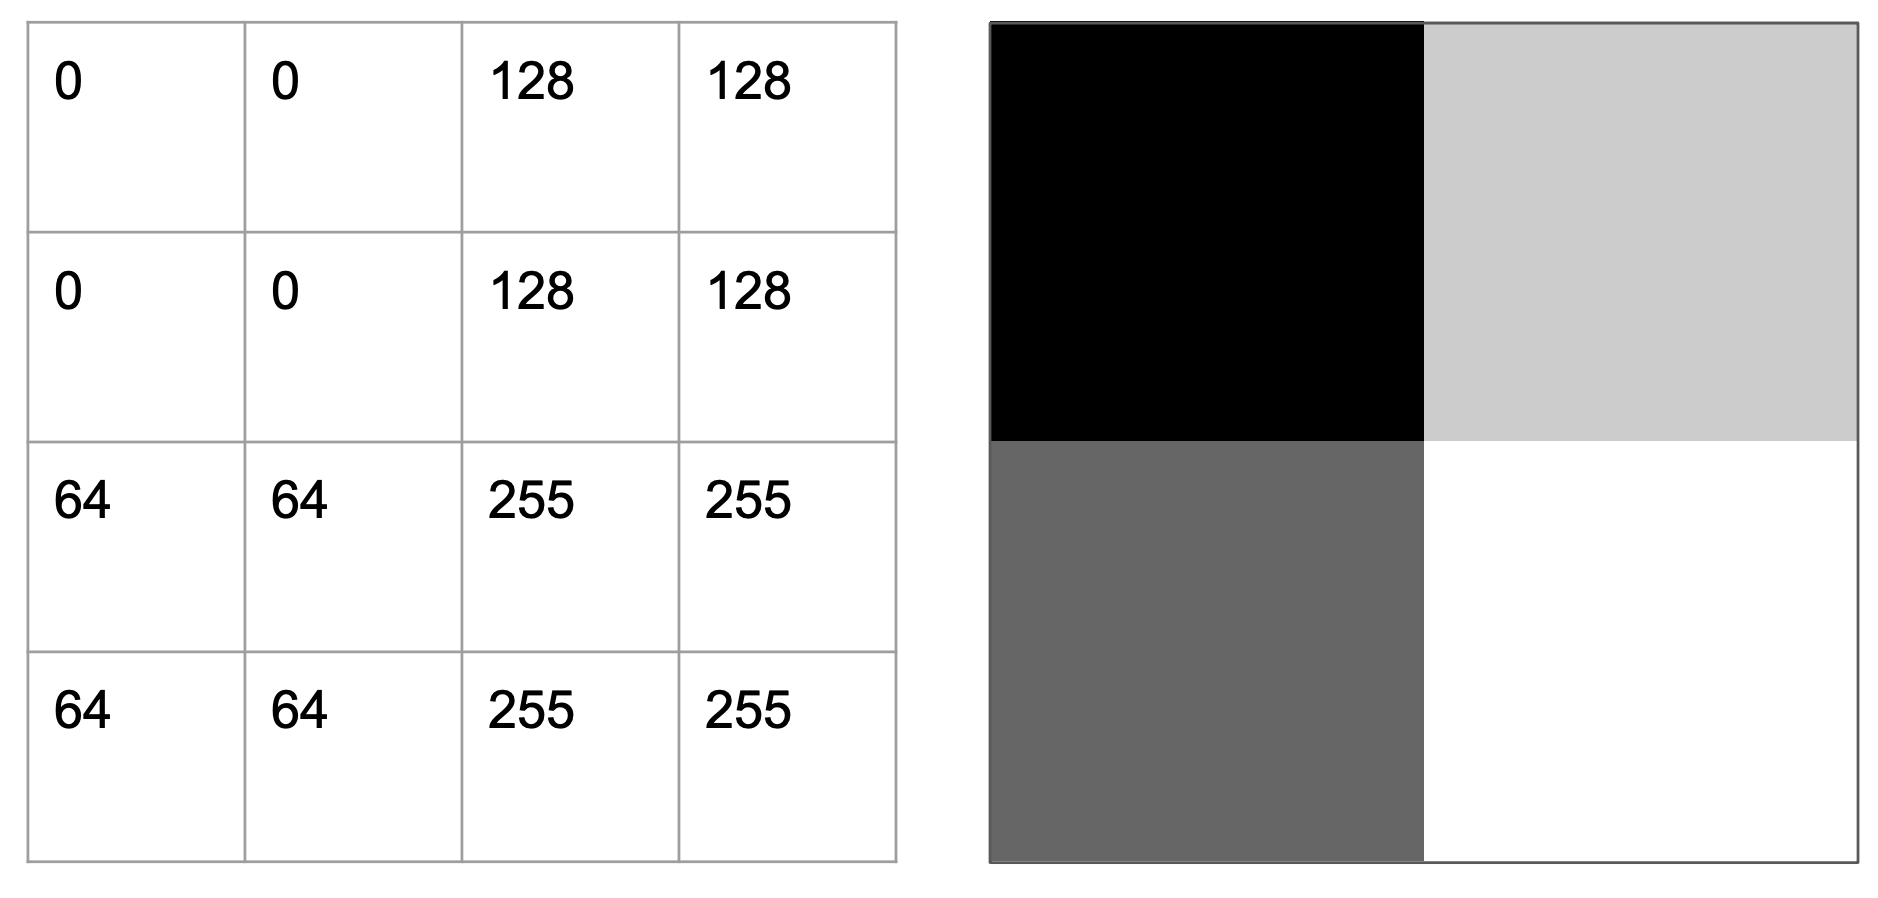
\includegraphics[width=7cm,keepaspectratio]{XX_Figures/Fig_GS.png}
	\caption{\footnotesize Cuatro escalas de grises con su respectivo valor numérico en la matriz izquierda}
	\label{fig:Fig_GS}
\end{figure}

\begin{figure}[p]
	\centering
	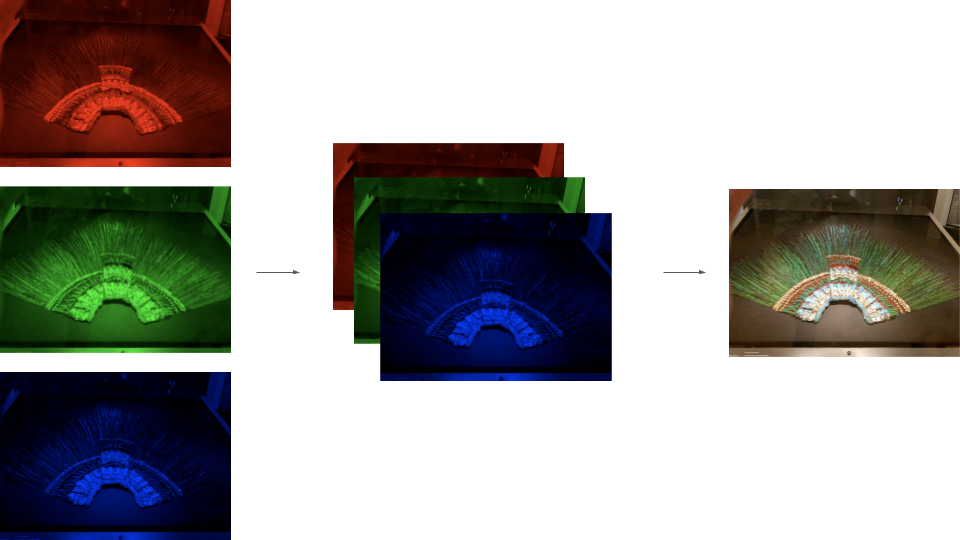
\includegraphics[width=10cm,keepaspectratio]{XX_Figures/Fig_RGB.png}
	\caption{\footnotesize Los tres canales de una imagen en RGB }
	\label{fig:Fig_RGB}
\end{figure}


\begin{figure}[p]
	\centering
	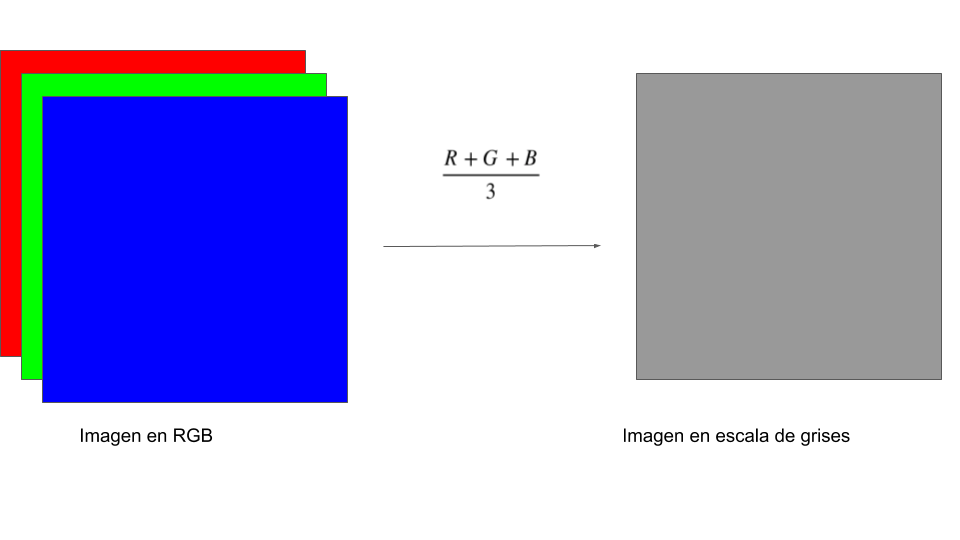
\includegraphics[width=7cm,keepaspectratio]{XX_Figures/Fig_RGBtoGS.png}
	\caption{\footnotesize Conversión de una imagen RGB a escala de grises por promediación}
	\label{fig:Fig_RGBtoGS}
\end{figure}

Una imagen está definida por una función bidimensional \textit{f(x,y)}, donde \textit{x} y \textit{y} son coordenadas espaciales; y la amplitud de \textit{f}  en cualquier par de coordenadas \textit{(x,y)} se llamada intensidad en cualquier punto de la imagen.
Si los valores de \textit{f} son valores finitos discretos, entonces podemos llamar a la imagen una imagen digital. Una imagen digital tiene número finito de elementos y cada uno de estos tiene una localización y valor; a estos elementos se les llaman píxeles \cite{GonzalezDigitalProcessing.pdf}.

Por lo general la mayoría de los píxeles toman valores de 0 a 255 (8 bits); en una imagen en escala de grises 0 representa el  negro y 255 representa blanco, un ejemplo se muestra en la Figura \ref{fig:Fig_GS}.

%----------------------------------------------------------------------------------------
\subsection{RGB}
\label{RGB}

Las imágenes representadas en un modelo RGB, consisten en tres componentes de imágenes como se muestra en la Figura \ref{fig:Fig_RGB}, uno por cada color primario (rojo, verde y azul); cuando estos tres colores alimentan un monitor produce una imagen a color. Considerando que cada uno de los tres canales (R,G,B) contiene 8 bits, al tener una imagen a color tendremos 24 bits de datos, el cuál nos da un posibilidad de tener 16,777,216 colores ($(2^8)^3 = 16,777,216$).\\

----------------------
\subsection{Escala de Grises}
\label{GS}

Una imagen en RGB puede ser convertida a escala de grises (GS) a través de varios métodos. El método más utilizado es por promediación como se muestra en la Figura \ref{fig:Fig_RGBtoGS} en el que los tres valores de los píxeles de los tres planos en la misma posición es sumado y dividido entre tres; esta operación se repite para todos los píxeles para obtener un solo plano.

%----------------------------------------------------------------------------------------
\subsection{Filtros Espaciales}
\label{Filtros_espaciales}

\begin{figure}[th]
	\centering
	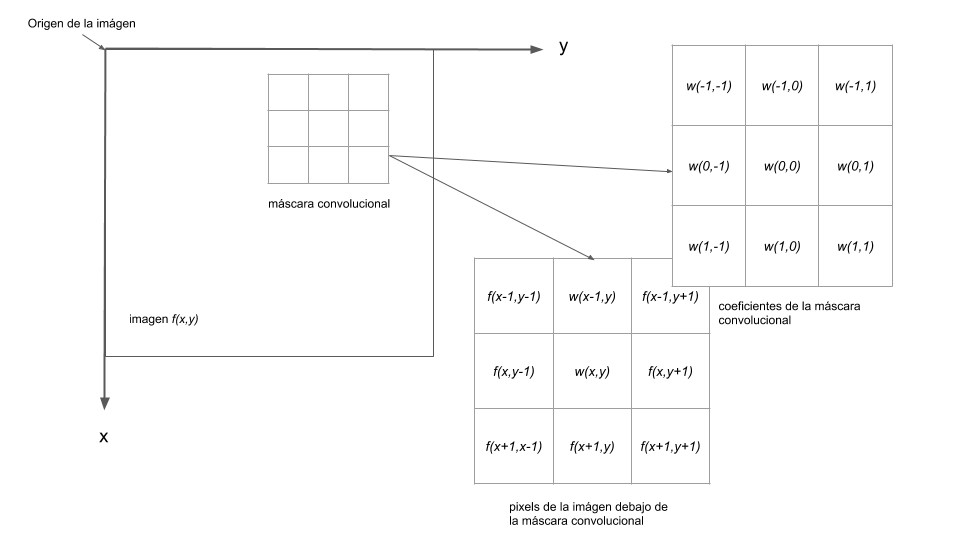
\includegraphics[width=13cm,keepaspectratio]{XX_Figures/Fig4_Convolucion.png}
	\caption{\footnotesize Mecánica del filtraje espacial. El dibujo ampliado muestra una imagen de 3 x 3 y la sección de la imagen que yace directamente bajo ella; la sección de la imagen se muestra desplazada respecto a la máscara para facilitar la legibilidad \cite{GonzalezDigitalProcessing.pdf}}
	\label{fig:Fig4_Convolucion}
\end{figure}

Las operaciones para el filtrado espacial se aplican directamente sobre los píxeles de una imagen como se muestra en la Figura \ref{fig:Fig4_Convolucion}. Para realizar el filtrado  se realiza un barrido de un núcleo (kernel) o máscara de convolución, sobre cada punto de la imagen \cite{GonzalezDigitalProcessing.pdf}. A las máscaras o filtros utilizados, también se le llaman comúnmente como máscaras convolucionales, ya que el proceso del filtrado lineal tiene similitud con el concepto en dominio de la frecuencia llamada convolución. En general, para un filtrado espacial lineal de una imagen \textit{f} de tamaño \textit{M} x \textit{N} con un kernel de tamaño \textit{m} x \textit{n}, la salida de nuestro filtrado está dada por la ecuación \ref{equ:Filtro_lineal}.

\begin{equation}
	\label{equ:Filtro_lineal}
	g(x,y) =  \sum_{s=-a}^{a}\sum_{t=-b}^{b}w(s,t)f(x+s,y+t).\\
\end{equation}

Donde \textit{a = (m-1)/2} y \textit{b = (n-1)/2}, y el filtrado debe ser aplicado para \textit{x = 0,1,2,...,M-1} y \textit{y = 0,1,2,...,N-1}. De esta manera aseguramos que la máscara sea aplicada a todos los píxeles de la imagen. 

Comúnmente para simplificar la notación y no enfocarse en las mecánicas implementadas por una máscara convolucional, solamente en la respuesta obtenida, se utiliza la ecuación \ref{equ:Filtro_lineal_simplicado}.

\begin{equation} 
\label{equ:Filtro_lineal_simplicado}
\begin{split}
R &= w_{1}z_{1} + w_{2}z_{2} + ... + w_{mn}z_{mn} \\
g(x,y) &=  \sum_{i=1}^{mn}w_{i}z_{i}.
\end{split}
\end{equation}

Donde \textit{w's} son los coeficientes de la máscara utilizada y \textit{z's} los valores de una imagen en escala de grises. Esta ecuación es usada más frecuentemente en la literatura de procesamiento de imágenes \cite{GonzalezDigitalProcessing.pdf}.

%-----------------------------------------------------------------------------------------%-----------------------------------------------------------------------------------------
\subsubsection{Sobel}
\label{Sobel}

\begin{figure}[th]
	\centering
	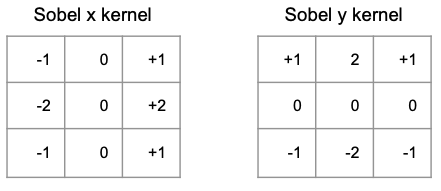
\includegraphics[width=5cm,keepaspectratio]{XX_Figures/Fig_Matrices_Sobel.png}
	\caption{\footnotesize Matrices del operador \textit{Sobel} para detectar bordes.}
	\label{fig:Fig_Matrices_Sobel}
\end{figure}

\begin{figure}[th]
	\centering
	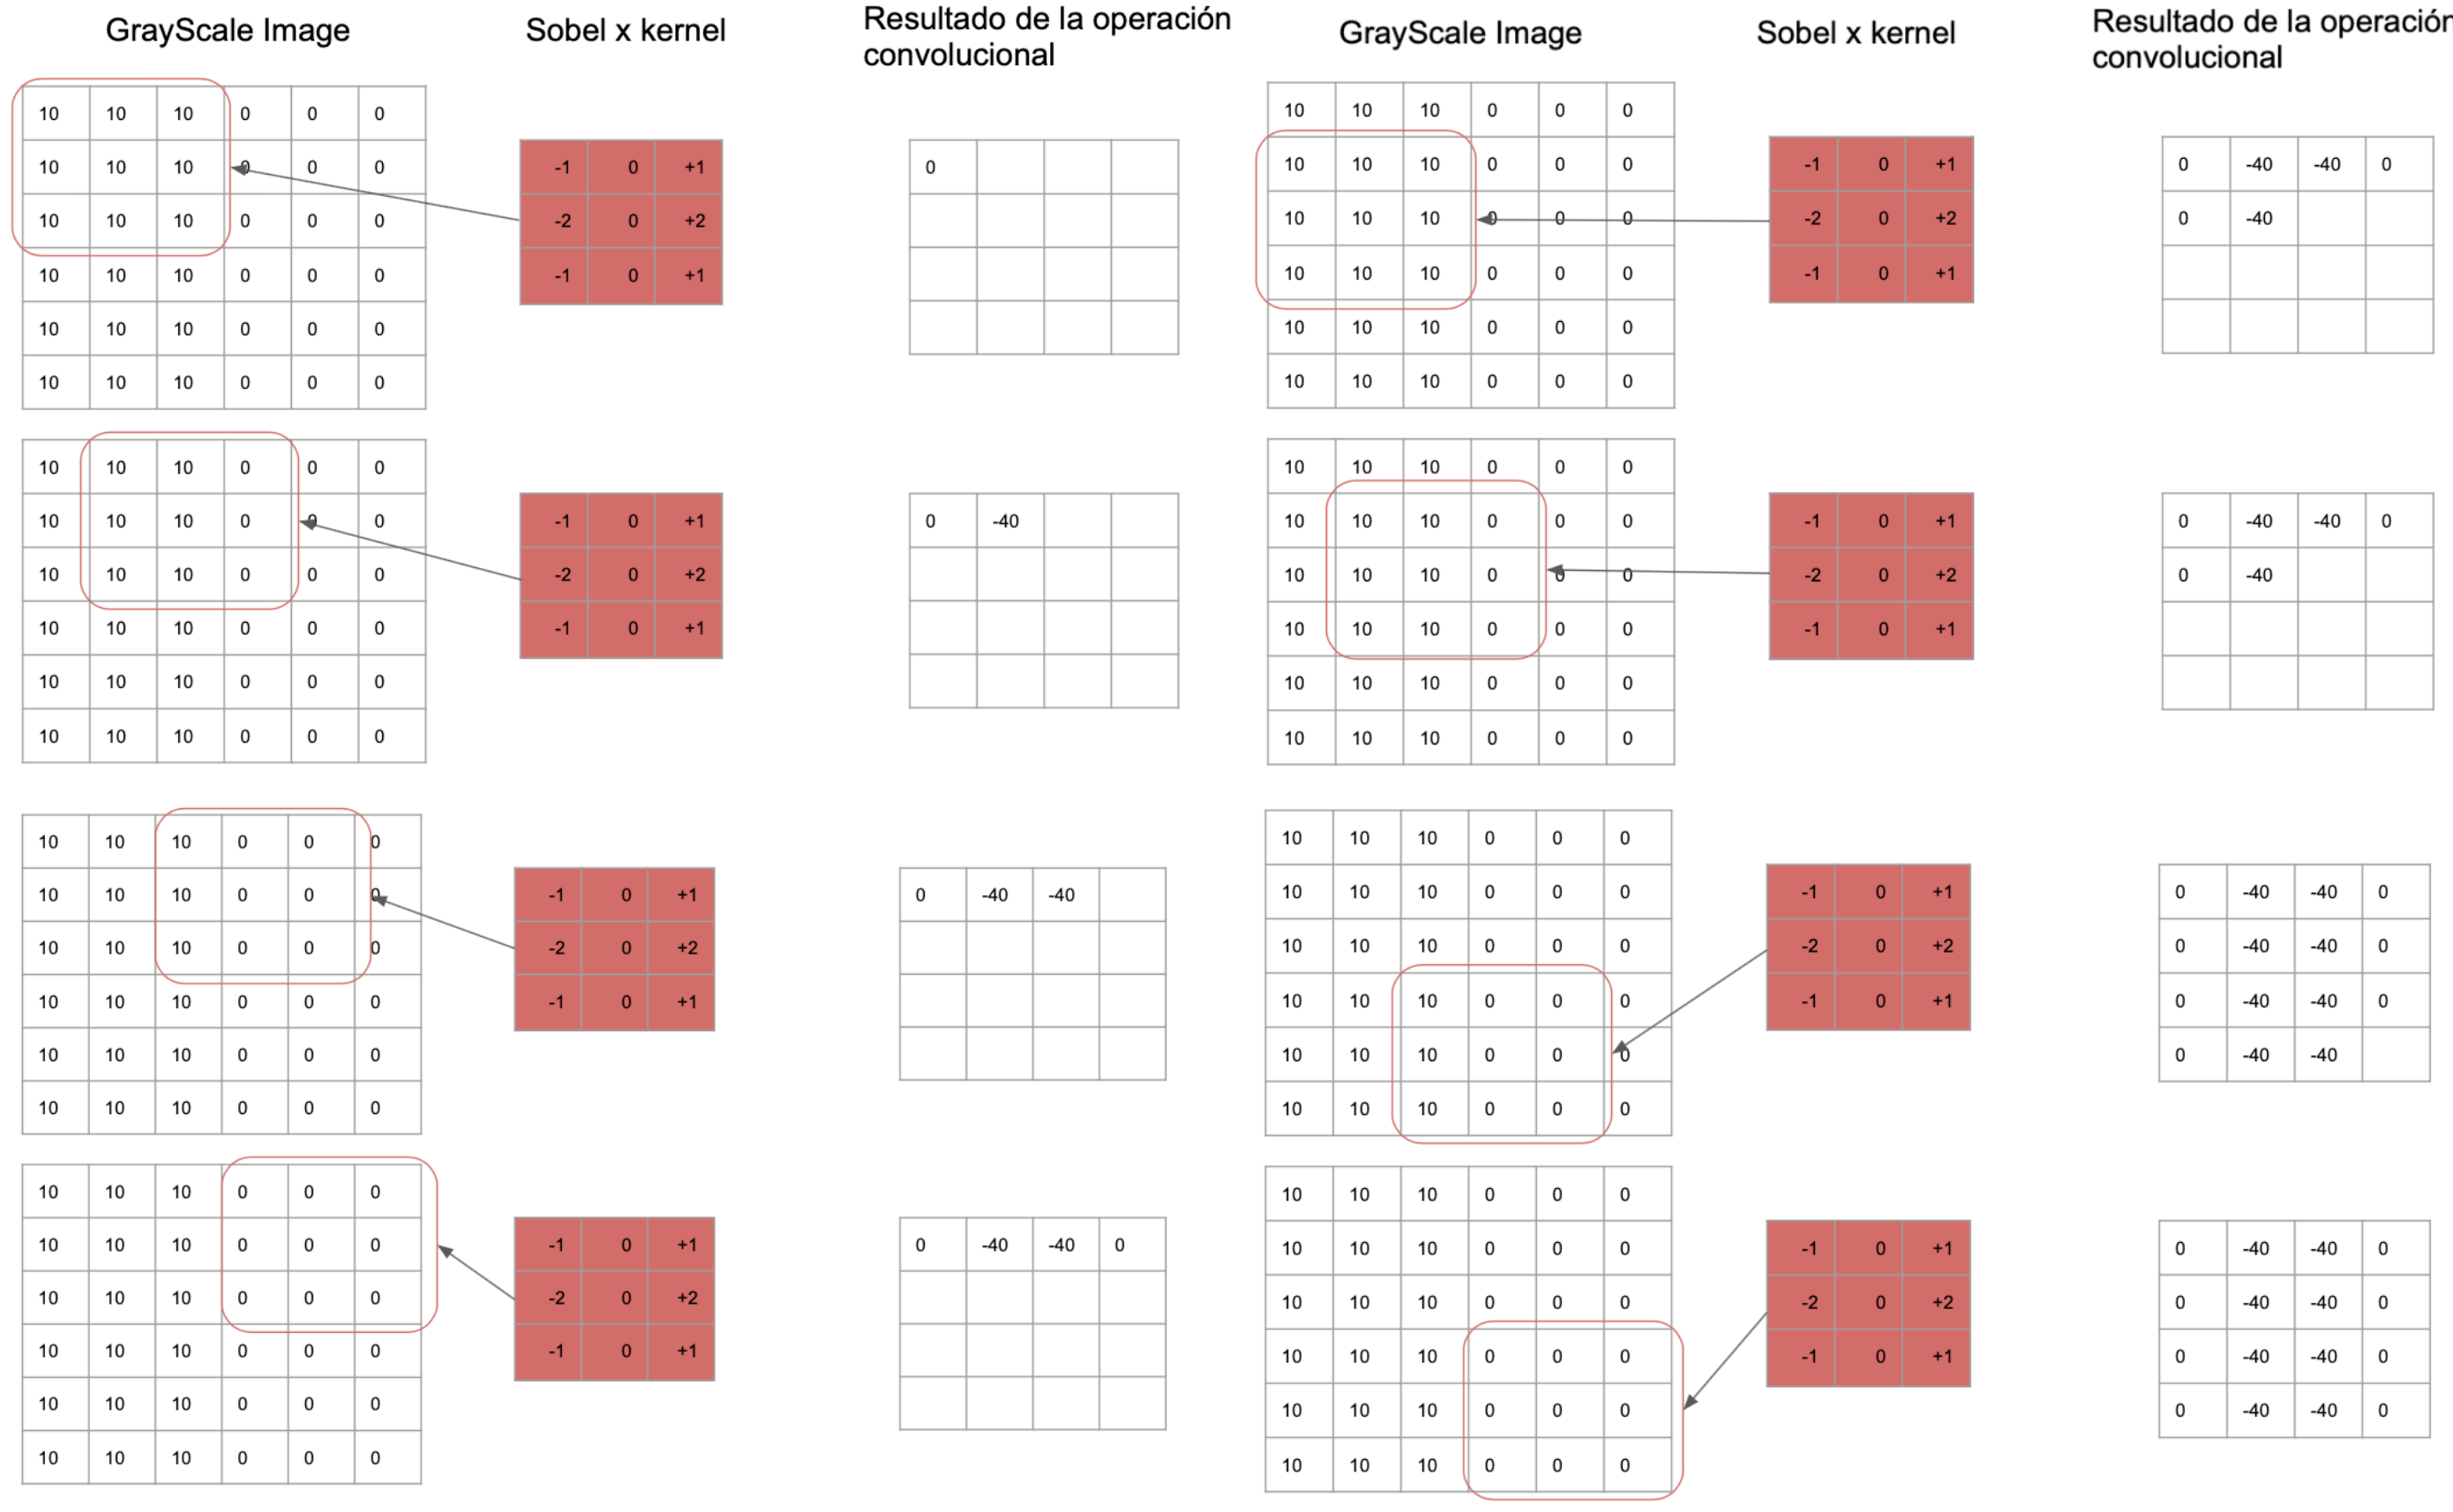
\includegraphics[width=17cm,keepaspectratio]{XX_Figures/Fig_Ejemplo_Sobelx.png}
	\caption{\footnotesize Resultados numéricos al aplicar un filtro \textit{Sobelx} sobre una imagen de 6 x 6}
	\label{fig:Fig_Ejemplo_Sobelx}
\end{figure}

\begin{figure}[th]
	\centering
	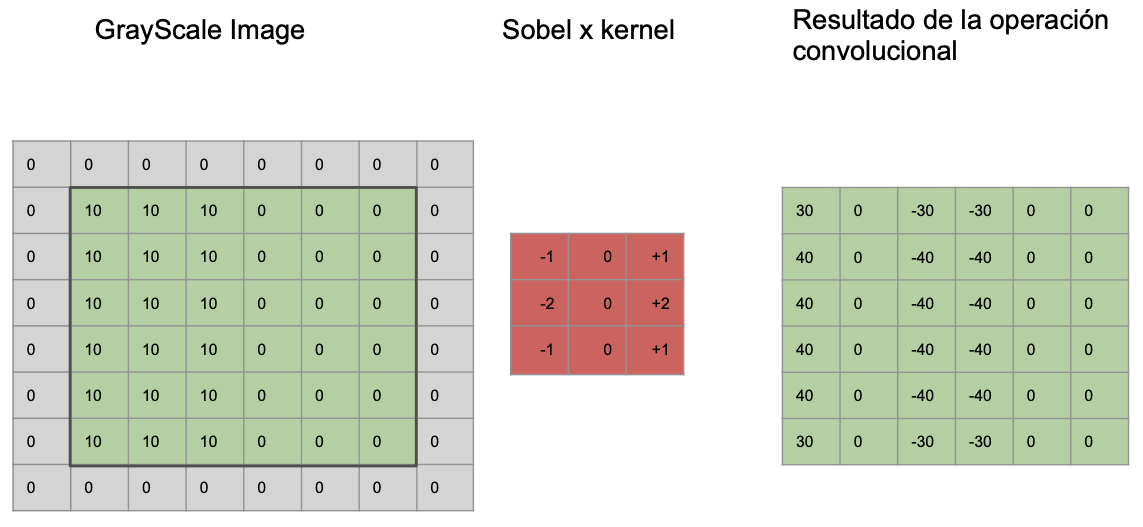
\includegraphics[width=10cm,keepaspectratio]{XX_Figures/Fig_Sobel_padding.png}
	\caption{\footnotesize Relleno de ceros alrededor de los bordes de la imagen}
	\label{fig:Fig_Sobel_padding}
\end{figure}

El operador Sobel es un filtro espacial que tiene como objetivo la detección de los bordes de los objetos en una imagen. Este filtro es utilizado comúnmente para detectar objetos en una imagen a través de los bordes; el operador utiliza un par de matrices de gradiente horizontal y vertical cuyas dimensiones son de 3 x 3 para las operaciones de detección de bordes \cite{Gupta2013SobelAlgorithm}. Estas matrices se muestran en la Figura \ref{fig:Fig_Matrices_Sobel} y en la Figura \ref{fig:Fig_Ejemplo_Sobelx} un ejemplo de cómo se van detectando los bordes utilizando las máscaras convolucionales del operador \textit{Sobely}. Podemos ver que al terminar una operación, el filtro se mueve una posición para seguir con el mismo procedimiento en una localización distinta; a este movimiento se le conoce comúnmente como paso (stride), el cual es el número de desplazamientos de píxeles sobre la matriz de píxeles. En el último paso de la Figura \ref{fig:Fig_Ejemplo_Sobelx} se observa que se obtiene una matriz con valores negativos; esto quiere decir que existe un borde en la imagen y este tiene dirección hacia la izquierda. Si en dado caso se quisiera obtener solamente el filtro \textit{Sobelx} sin dirección, simplemente se obtiene el valor absoluto de todos los píxeles.
Nótese que al aplicar el operador \textit{Sobel} se reduce el tamaño de la imagen resultante. Para evitar este problema, se agrega un relleno (padding) en los bordes de la imagen como se muestra en la Figura \ref{fig:Fig_Sobel_padding}, para que al momento de aplicar nuestro operador y de hacer el barrido por toda la imagen, se obtenga la misma cantidad de píxeles \cite{LaplacianEdgeFilter}. Este relleno es aplicado en varios filtros convolucionales para obtener la misma cantidad de píxeles en los resultados.


%-----------------------------------------------------------------------------------------
\subsubsection{Laplaciano}
\label{Laplaciano}

\begin{figure}[th]
	\centering
	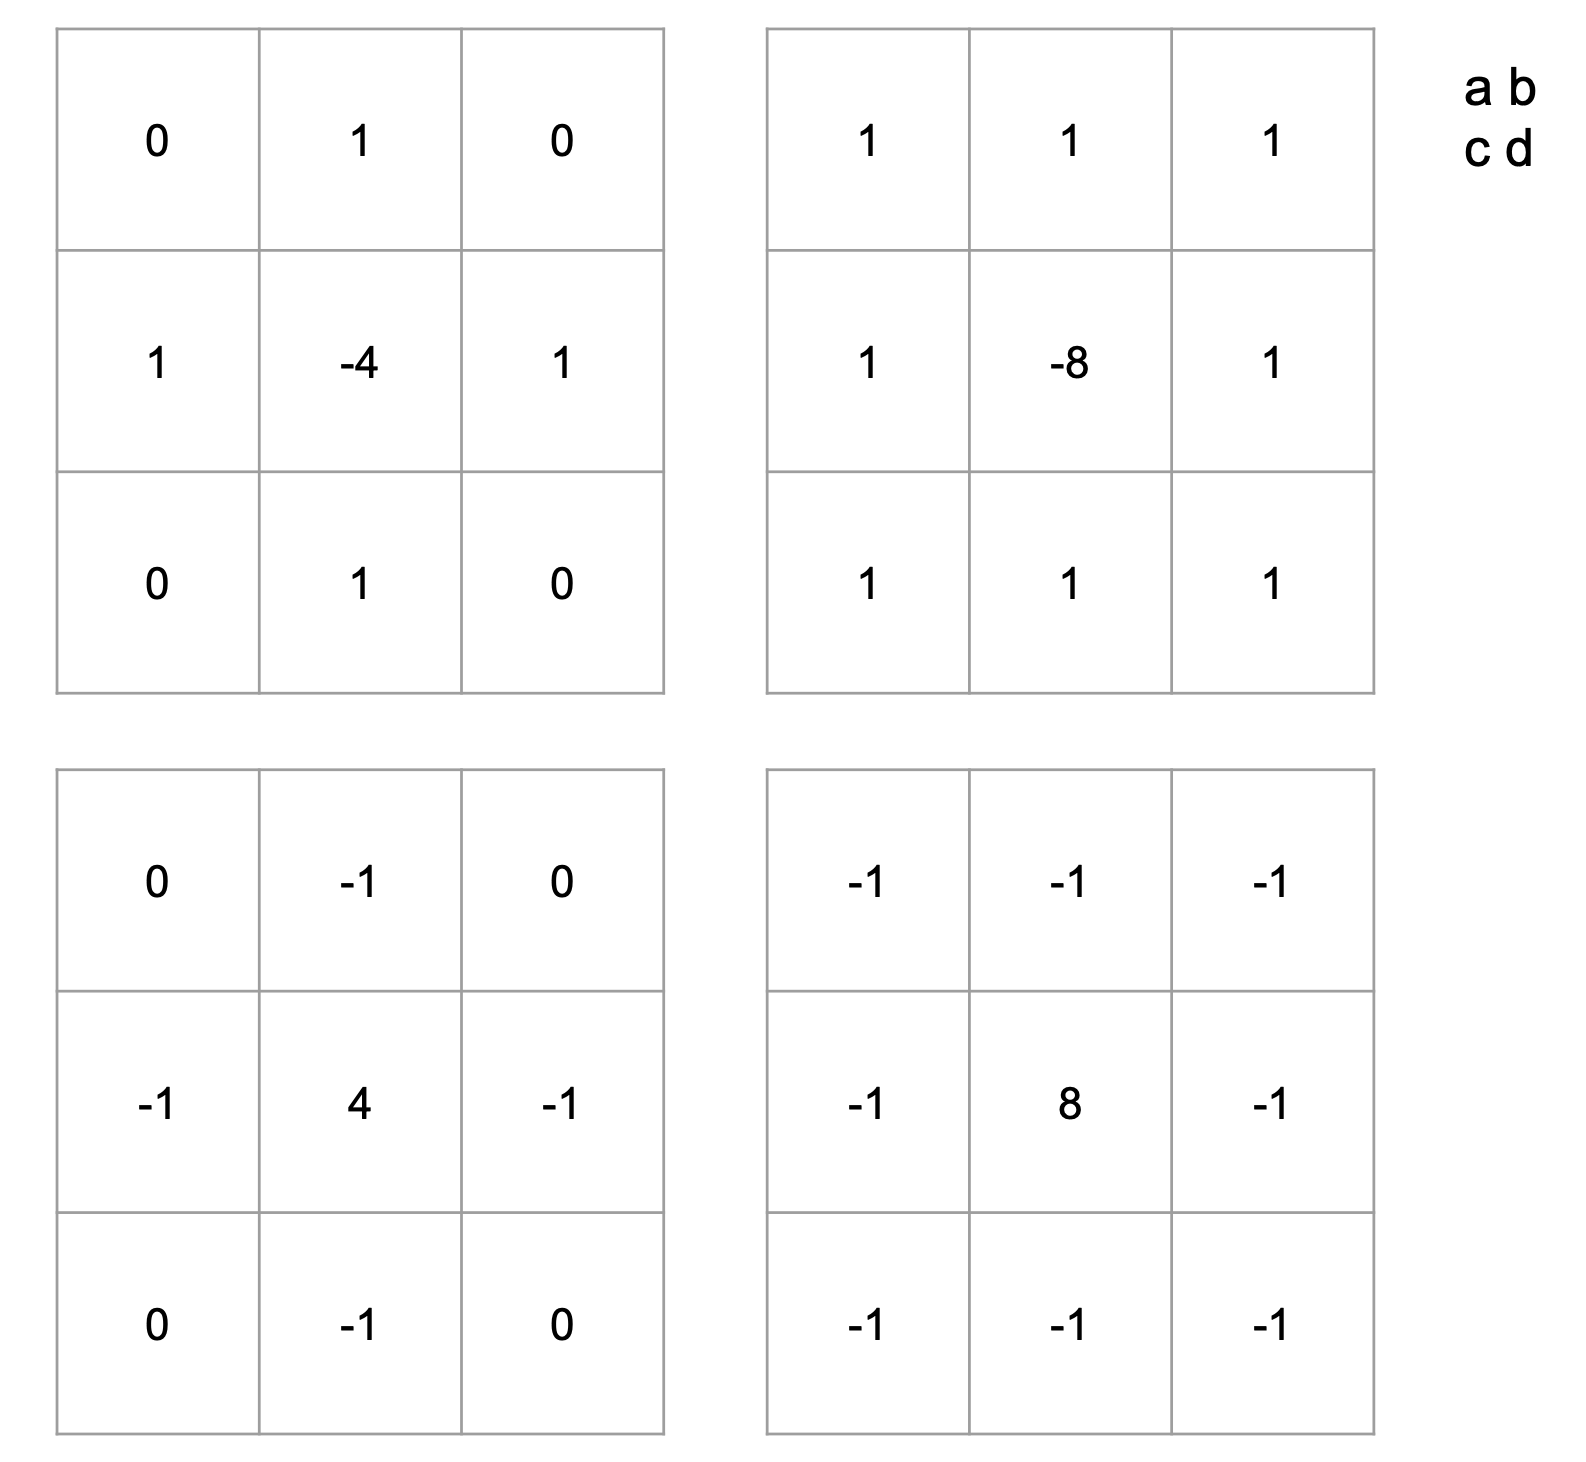
\includegraphics[width=5cm,keepaspectratio]{XX_Figures/Fig_Filtros_Laplacianos.png}
	\caption{\footnotesize Filtros Laplacianos con diferentes cualidades e implementaciones.}
	\label{fig:fig_filtros_laplacianos}
\end{figure}

El filtro Laplaciano es uno de los filtros utilizados con el objetivo de agudizar una imagen y así resaltar detalles que no se lograban ver, posiblemente porque la imagen estaba borrosa.

En la Figura \ref{fig:fig_filtros_laplacianos} podemos ver 4 máscaras convolucionales Laplacianos comúnmente utilizados. En la Figura \ref{fig:Fig_Ejemplo_Laplaciano} se puede notar en la imagen del centro el resultado de aplicar un kernel Laplaciano sobre una imagen y en la imagen de la derecha se observa como la imagen se agudiza y se notan más detalles gracias a la suma escalada del filtro Laplaciano y la imagen original.

\begin{figure}[th]
	\centering
	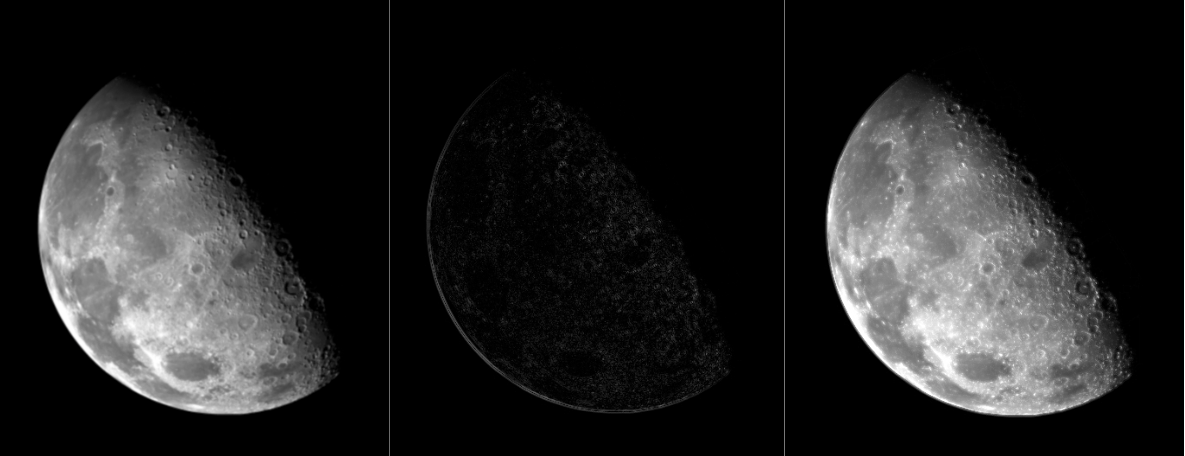
\includegraphics[width=10cm,keepaspectratio]{XX_Figures/Fig_Ejemplo_Laplaciano.png}
	\caption{\footnotesize A la izquierda una imagen de la Luna, al centro el resultado de aplicarle el filtro Laplaciano c de la Figura \ref{fig:fig_filtros_laplacianos} y a su derecha la suma escalada de las dos imágenes previamente mencionadas.}
	\label{fig:Fig_Ejemplo_Laplaciano}
\end{figure}

%----------------------------------------------------------------------------------------
%-----------------------------------------------------------------------------------------
\subsubsection{Kirsch}
\label{Kirsch}

\begin{figure}[th]
	\centering
	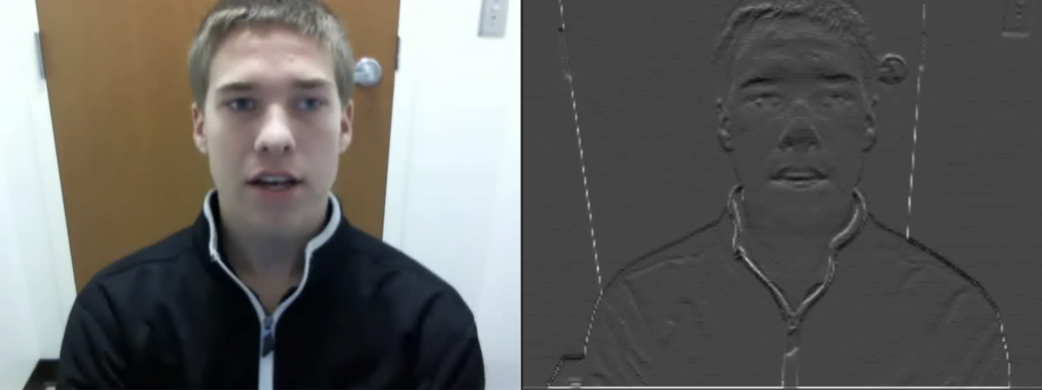
\includegraphics[width=11cm,keepaspectratio]{XX_Figures/Fig_Ejemplo_Kirsch.png}
	\caption{\footnotesize Aplicación del filtro Kirsch.}
	\label{fig:Fig_Ejemplo_Kirsch}
\end{figure}

El filtro Kirsch es un operador detector de bordes que encuentra el borde más significativo en ocho direcciones predeterminadas. La magnitud del borde se obtiene explorando el valor de los píxeles alrededor de ese píxel. Si todos los píxeles en el vecindario tienen casi el mismo valor, entonces probablemente no haya un borde en ese punto. Sin embargo, si algunos de los píxeles alrededor tienen valores mayores que los demás entonces, existe la probabilidad de que haya un borde en ese punto \cite{Kalaiselvi2017ModifiedSegmentation}. El algoritmo Kirsch utiliza un kernel de 3 × 3 y  lo rota 45 grados para así obtener 8 direcciones como se muestra a continuación. 
\begin{align*}
E &= \begin{bmatrix}
-3 & -3 & 5 \\
-3 & 0 & 5 \\
-3 & -3 & 5 
\end{bmatrix},
& 
N &= \begin{bmatrix}
5 & 5 & 5 \\
-3 & 0 & -3 \\
-3 & -3 & -3
\end{bmatrix},
& 
W &= \begin{bmatrix}
5 & -3 & -3 \\
5 & 0 & -3 \\
5 & -3 & -3
\end{bmatrix},
&
S &= \begin{bmatrix}
-3 & -3 & -3 \\
-3 & 0 & -3 \\
5 & 5 & 5
\end{bmatrix},
&\\
NE &= \begin{bmatrix}
-3 & 5 & 5 \\
-3 & 0 & 5 \\
-3 & -3 & -3
\end{bmatrix},
&
NW &= \begin{bmatrix}
5 & 5 & -3 \\
5 & 0 & -3 \\
-3 & -3 & -3
\end{bmatrix},
&
SW &= \begin{bmatrix}
-3 & -3 & -3 \\
5 & 0 & -3 \\
5 & 5 & -3
\end{bmatrix},
&
SE &= \begin{bmatrix}
-3 & -3 & -3 \\
-3 & 0 & 5 \\
-3 & 5 & 5
\end{bmatrix},
\end{align*}


\begin{figure}[th]
	\centering
	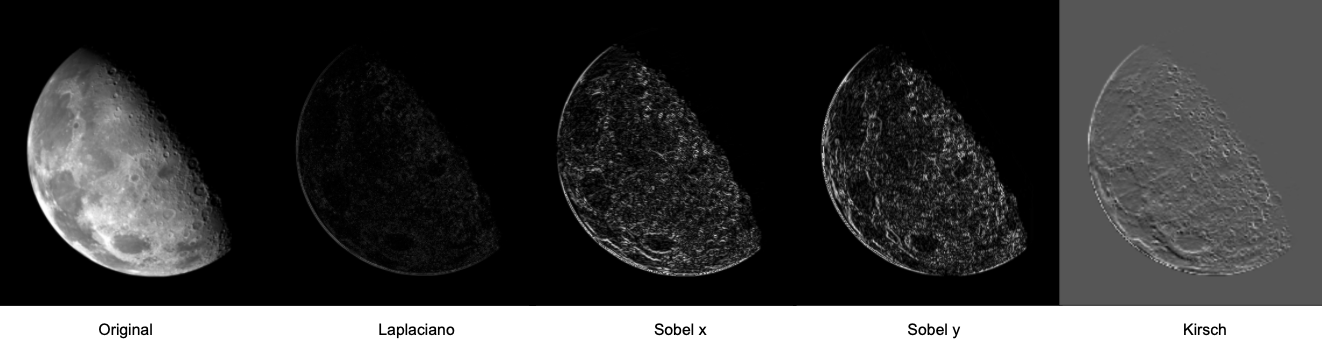
\includegraphics[width=17cm,keepaspectratio]{XX_Figures/Fig_Comparacion_Filtros.png}
	\caption{\footnotesize Comparación de filtros convolucionales para agudización y detección de bordes.}
	\label{fig:Fig_Comparacion_Filtros}
\end{figure}


En la Figura \ref{fig:Fig_Ejemplo_Kirsch}, se puede observar la utilidad de este operador convolucional después de convertir la imagen de RGB a escala de grises y en la Figura \ref{fig:Fig_Comparacion_Filtros} se puede comparar los resultados al aplicar los filtros convolucionales para bordes y agudizamiento mencionados anteriormente. Se debe resaltar que para aplicar todos los filtros mencionados anteriormente, es necesario tener la imagen en escala de grises.\\

Estos filtros son utilizados para resaltar u obtener diferentes características en imágenes, dependiendo de la tarea que se desee realizar.

%-----------------------------------------------------------------------------------------
\subsubsection{Flujo óptico}
\label{OpticalFlow}

El flujo óptico está definido como el movimiento aparente que tiene cada píxel en una imagen. Si se desea analizar el movimiento humano, las expresiones y los gestos, una sola imagen es muy poca información para entender a que clase pertenece un gesto humano. Con el flujo óptico (optical flow) podemos obtener imágenes que representan el movimiento del contexto de la escena en relación con un observador ya que utiliza dos frames que contienen objetos en diferentes posiciones de la imagen y pueden ser utilizados para extraer características temporales.
En la Figura \ref{fig:Fig_OpticalFlow}, se observa un ejemplo del funcionamiento del OpticalFlowX y OpticalFlowY.

\begin{figure}[th]
	\centering
	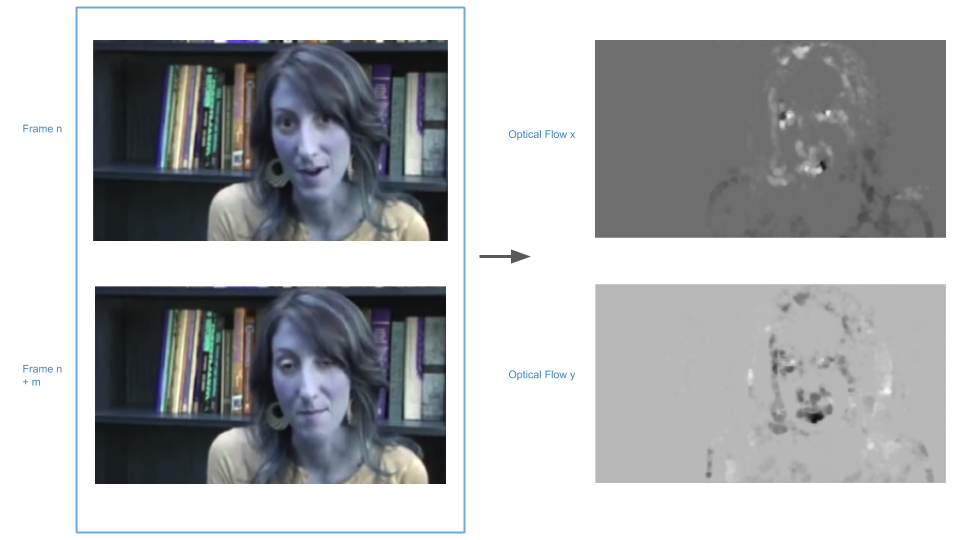
\includegraphics[width=14cm,keepaspectratio]{XX_Figures/Fig_OpticalFlow.png}
	\caption{\footnotesize Flujo óptico de dos imágenes separadas m cantidad de frames.}
	\label{fig:Fig_OpticalFlow}
\end{figure}

%----------------------------------------------------------------------------------------
%----------------------------------------------------------------------------------------
\section{Redes neuronales artificiales}
\label{RNA}
%----------------------------------------------------------------------------------------
Las redes neuronales artificiales (RNA) tratan de emular ciertas características del sistema nervioso, en la cual a través de un estímulo, la neurona brinda una respuesta a ese estímulo. \cite{Chernyatin1968NNDesign} Una red neuronal estándar consiste en conectar procesadores de información llamados neuronas que van produciendo una secuencia de activaciones con un valor real. Las neuronas pueden ser activadas a través de sensores que perciben el ambiente y otras se activan a través de conexiones ponderadas de neuronas previamente activadas. 

Hay tres elementos básicos de un modelo neuronal. El primer elemento es un conjunto de sinapsis, cada una caracterizada con un propio peso o resistencia. A diferencia del peso de una sinapsis cerebral, el peso sináptico de una RNA puede incluir valores reales negativos y positivos. El segundo elemento es un sumador que ayuda a sumar las señales de entrada ponderadas por sus respectivas fuerzas sinápticas de la neurona. El último elemento es una función de activación para limitar la amplitud de la salida de una neurona \cite{Hawkin2014IntriguingFergus}. Varios avances se han logrado al desarrollar programas inteligentes; con las RNAs podemos resolver de manera exitosa problemas como reconocimiento de patrones, predicción, optimización, memorias asociativas y control \cite{Majumder2015ArtificialNetwork}.
	
En años recientes las redes neuronales profundas artificiales (DNN) han mostrado un gran desempeño en reconocimiento de patrones y el aprendizaje máquina. El aprendizaje profundo y no profundo se distinguen por las diferentes profundidades de rutas que generan posibles vínculos de aprendizaje \cite{Schmidhuber2015DeepOverview}. Dependiendo del problema que se esté enfrentando, de cómo están conectadas las neuronas y de las capas que tengamos es cómo se determinará la función y el comportamiento de nuestra arquitectura de red neuronal \cite{Chernyatin1968NNDesign}.
%----------------------------------------------------------------------------------------
\subsection{Perceptrón Multicapa}
\label{MLP}
%----------------------------------------------------------------------------------------
Se ha demostrado que el uso de la perceptrón multicapa (MLP) es una alternativa efectiva para aproximar prácticamente cualquier función uniforme medible ya que a diferencia de otras técnicas convencionales estadísticas, la perceptrón multicapa no realiza suposiciones previas sobre la distribución de los datos. De igual manera puede modelar funciones altamente no lineales y puede ser entrenada para generalizar con precisión cuando se le presentan datos nunca antes vistos \cite{Gardner1998ArtificialSciences}.\\

La MLP consiste en un sistema de neuronas interconectadas como se muestra en la Figura \ref{fig:fig2_MLP}. Cada una de las neuronas están conectadas por pesos y señales de salida las cuales son una función de la suma de las entradas a la neurona modificada por una función de activación. Es la superposición de muchas funciones de transferencia no lineales simples lo que le da a la MLP la capacidad de aproximar funciones no lineales. Si la función de transferencia de la MLP es lineal entonces solo podrá modelar funciones lineales. La salida de las neuronas es escalada por el peso de conexión de la siguiente neurona en la siguiente capa de la red. Una MLP puede llegar a tener una o varias capas ocultas y al final una capa de salida. Las entradas y las salidas de la MLP pueden ser representadas por vectores simples \cite{Gardner1998ArtificialSciences}. \\

\begin{figure}[th]
	\centering
	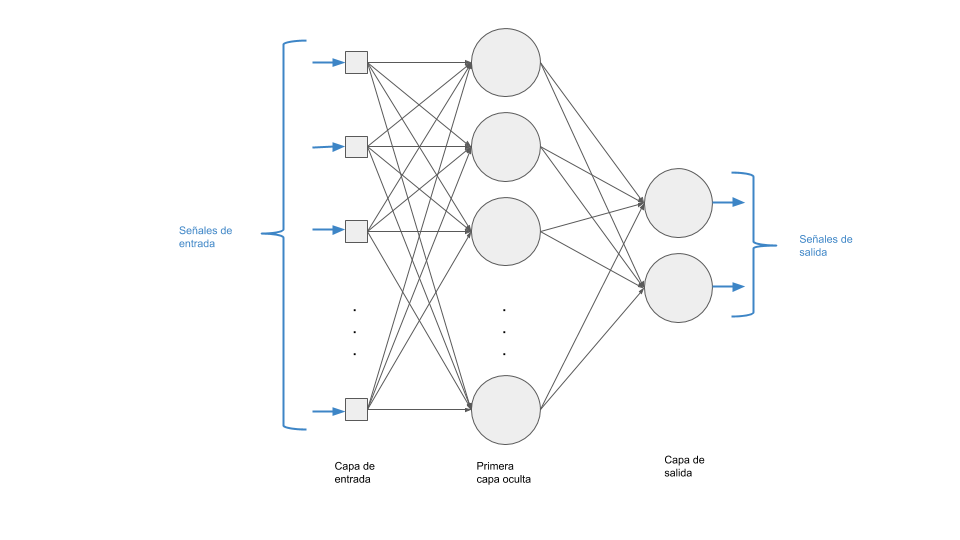
\includegraphics[width=14cm,keepaspectratio]{XX_Figures/fig2_MLP.png}
	\caption{\footnotesize MLP con dos señales de salida.}
	\label{fig:fig2_MLP}
\end{figure}

La MLP tiene la capacidad de aprender a través del entrenamiento, el cual consiste en una serie de entradas asociadas con su vector de salida y los pesos de la red se van ajustando hasta que el mapeo entrada-salida deseado ocurra; para lograrlo es necesario presentarle repetidamente a la red los datos de entrenamiento. Es por esto que la MLP tiene el objetivo de crear una función capaz de predecir el valor correspondiente a una entrada valida después de haber visto una serie de ejemplos en los datos de entrenamiento. Si logramos obtener conjuntos adecuados de pesos y funciones de transferencia, se ha demostrado que la MLP puede aproximarse a cualquier función uniforme y medible entre los vectores de entrada y salida \cite{Caille1980EtudeThymie}. Para lograr que la MLP obtenga pesos y funciones de transferencia que logren la generalización cuando se le presentan datos nunca antes vistos, es necesario entrenarla con datos adecuadamente representativos. Por esta razón el buen funcionamiento de la MLP depende en gran parte de los datos de entrenamiento. 

Por lo general en la etapa de entrenamiento, puede que la salida de la MLP no sea igual a la salida deseada, por lo que se calcula una señal de error definida como la diferencia entre la salida deseada y la salida real; esta señal es usada en el entrenamiento para determinar en qué grado se deben ajustar los pesos en la red y de esta manera el error pueda ser reducido. Por lo anterior, el objetivo del entrenamiento es encontrar la combinación de pesos el cual nos dará el punto mínimo para la superficie del error. 

%El algoritmo de retropropagación (back-propagation algorithm) es el algoritmo más sencillo computacionalmente para entrenar una MLP. Este algoritmo ocupa el procedimiento del gradiente descendiente para tratar de encontrar el mínimo global de la superficie del error y los pasos que sigue se resumen a continuación:%

%\begin{enumerate}
%        \item Inicializar los pesos de la red.
%    \item Presentar el primer vector de entrada del conjunto de entrenamiento a la red.
%    \item Propagar el vector de entrada a través de la red para obtener una salida.
%    \item Calcular la señal de error comparando la salida actual con la salida deseada.
%    \item Propagar la señal de error hacia atrás a través de la red (Figura \ref{fig:fig1_Senal_de_error}).
%    \item Ajustar los pesos para minimizar el error global.
%    \item Repetir los pasos 2-7 con el siguiente vector de entrada, hasta que el error global sea satisfactoriamente pequeño.
%\end{enumerate}

%\begin{figure}[th]
%	\centering
%	\includegraphics[width=11cm,keepaspectratio]{XX_Figures/%fig1_Senal_de_error.png}
%	\caption{\footnotesize Retropropagación de la señal de %error en una MLP.}
%	\label{fig:fig1_Senal_de_error}
%\end{figure}

\begin{figure}[th]
	\centering
	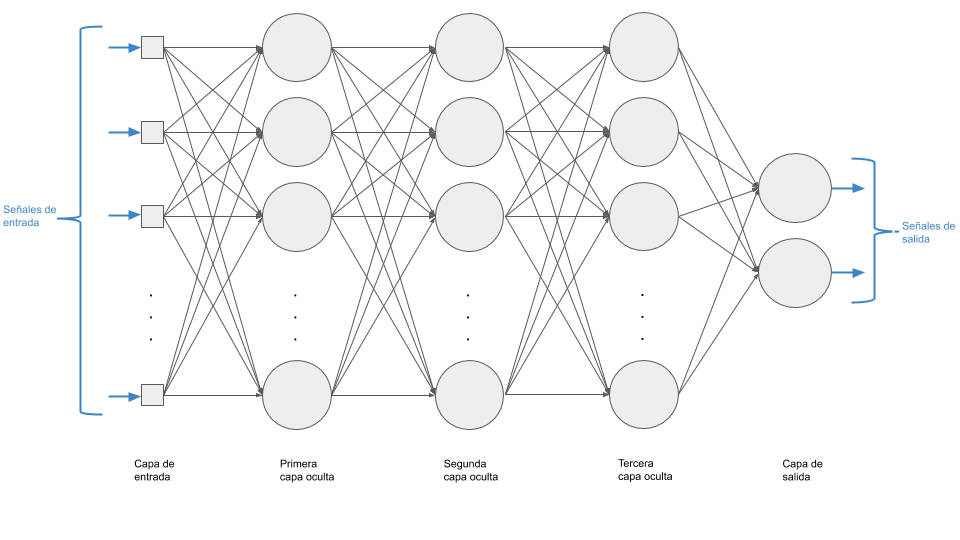
\includegraphics[width=16cm,keepaspectratio]{XX_Figures/fig3_MLP_profunda.png}
	\caption{\footnotesize MLP con tres capas ocultas y dos señales de salida.}
	\label{fig:fig3_MLP_profunda}
\end{figure}

%En este algoritmo los pesos de la red se adaptan después de que cada patrón ha sido presentado y a este método  se le conoce como on-line training; es un método en el cual la los datos se presentan de manera secuencial y es usado para actualizar nuestro modelo para futuros datos. Esta manera de entrenar es comúnmente utilizada para adaptar dinámicamente nuestro modelo a nuevos patrones o cuando los datos por sí mismos son generados en función del tiempo. Otra alternativa es conocida como batch training en la que la suma de todos los patrones es utilizada para actualizar los pesos de la red. De igual forma es necesario el paso de varias iteraciones de entrenamiento para que la red alcance un error satisfactoriamente bajo. El entrenamiento de la red no necesariamente debe terminar cuando se haya alcanzado un error global bajo deseado; también puede finalizar cuando en un conjunto de pruebas independiente, se haya alcanzado un desempeño satisfactorio.%
	
%El algoritmo de retropropagación contiene dos parámetros; uno es la tasa de aprendizaje (learning rate) el cuál controla qué tanto se debe cambiar el modelo en respuesta al error estimado cada vez que los pesos de la red es actualizado. Si el learning rate es muy pequeño entonces puede que el entrenamiento tome bastante tiempo en finalizar, en cambio si es muy grande entonces puede que el error de la red cambie erráticamente debido a grandes cambios en los pesos, resultando en la posibilidad de saltar sobre el error mínimo global. El segundo parámetro es el momentum el cual ayuda a acelerar el entrenamiento ya que en dado caso de que quedemos atrapados en un mínimo local y eso nos haga pensar de que hemos alcanzado un mínimo global, el  momentum toma un valor del 0 al 1, si es 1 o cercano, acelera el tamaño de los pasos tomados para poder salir de un mínimo local.%

\subsection{Perceptrón Multicapa Profunda}
\label{MLP_Profunda}

Si la cantidad de capas ocultas es mayor a tres (incluyendo capa de entrada y capa de salida), nuestra MLP califica como una perceptrón multicapa profunda (deep MLP) como se muestra en la Figura \ref{fig:fig3_MLP_profunda}, ya que cada capa contiene características de las señales de entrada con diferente nivel de abstracción; esto sucede porque cada capa de neuronas se entrena en un conjunto distinto de características basadas en la salida de la capa  anterior. Por esta razón, cuando más capas ocultas se tengan, más complejas serán las características que las neuronas pueden reconocer, ya que agregan y combinan características de las capas anteriores. Estrictamente se puede definir como una perceptrón multicapa profunda cuando se tiene más de una capa oculta.
	

%----------------------------------------------------------------------------------------
\subsection{Redes Neuronales Convolucionales}
\label{CNN}
%----------------------------------------------------------------------------------------
Este tipo de arquitectura de red neuronal profunda está inspirado por el mecanismo de percepción visual de los mamíferos y la principal razón es porque la corteza visual de los mamíferos consiste en conjunto de capas con células simples y células complejas; a medida que una imagen es procesada por la corteza visual, se detectan características progresivamente más ricas de la imagen. Las redes neuronales convolucionales (CNNs) consisten de conjuntos de capas convolucionales (convolutional layers) las cuáles se asimilan a las células simples, y conjuntos de capas de agrupación (pooling layers) que asimilan a las células complejas. Se ha demostrado que las CNNs aprenden progresivamente características de nivel superior en forma de filtros en las capas convolucionales \cite{Lecun2015DeepLearning}.\\

Las CNNs son particularmente adecuadas para manejar datos con un cierta estructura de información, tales como señales en audio en la cual la estructura está en una dimensión (vector simple), imágenes en dos dimensiones (una matriz de píxeles) y videos en tres dimensiones (varias matrices de píxeles). La estructura con la cual vamos a manejar los datos puede ayudar a mejorar el desempeño de nuestro modelo. En el caso de las MLPs con el objetivo de aprender a través de los datos de entrenamiento, nos vemos forzados convertir la estructura de nuestros datos (ej. Una matriz) a un vector simple.\\

\begin{figure}[th]
	\centering
	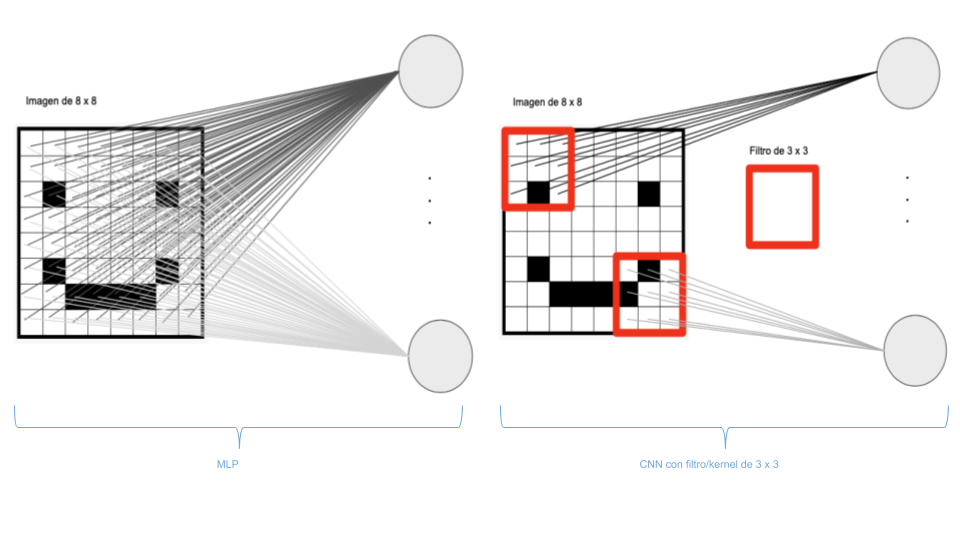
\includegraphics[width=13cm,keepaspectratio]{XX_Figures/Fig_Comparacion_MLP_CNN.png}
	\caption{\footnotesize Comparación de la conectividad de las neuronas entre una MLP y una CNN}
	\label{fig:Fig_Comparacion_MLP_CNN}
\end{figure}

Al igual que la MLP mencionada en el capítulo \ref{MLP}, las redes neuronales convolucionales, están conformadas de neuronas con pesos entrenables y biases. Cada neurona recibe varias entradas y se repite el mismo procedimiento; pero a comparación con la MLP en la que todas las neuronas de alguna capa \textit{n} están completamente interconectadas con la capa \textit{n-1} (Figura \ref{fig:fig3_MLP_profunda}), a cada neurona de la CNN se le conectan algunas neuronas cercanas de la capa anterior como se muestra en la Figura \ref{fig:Fig_Comparacion_MLP_CNN} y un mismo grupo de pesos es utilizado para cada neurona de salida, reduciendo considerablemente la cantidad de operaciones que se necesitan como se muestra en la Figura \ref{fig:Fig_Compartiendo_pesos} ya que las neuronas comparten parámetros y por lo tanto se requieren menos requerimientos computacionales.\\

\begin{figure}[th]
	\centering
	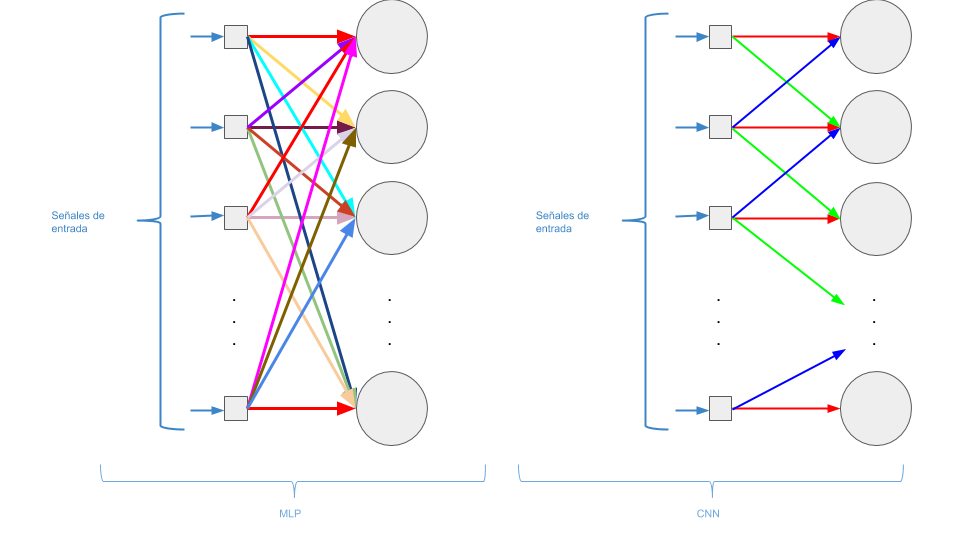
\includegraphics[width=14cm,keepaspectratio]{XX_Figures/Fig_Compartiendo_pesos.png}
	\caption{\footnotesize Comparación de pesos entre una MLP y una CNN.}
	\label{fig:Fig_Compartiendo_pesos}
\end{figure}

%En el siguiente ejemplo se puede notar claramente la reducción de parametros utilizados entre una CNN y una MLP:
%Si nostros tenemos una imagen en RGB de 224 x 224 \textit{pixeles} , entonces tendremos como entrada \textit{x = 224*224*3}, y deseamos tener en la siguiente capa 224,224\\


Este patrón de conexión tiene sentido cuando se pueden extraer características de los datos de manera espacial tal y como funciona una convolución explicado en el Capítulo \ref{Filtros_espaciales}, en la cual se ocupaban las operaciones convolucionales para extraer características de imágenes digitales como resaltar los bordes de los objetos, agudizar la imagen, etc. De igual forma las operaciones convolucionales en las CNNs tienen los mismos atributos mencionados anteriormente en el Capítulo \ref{Filtros_espaciales}, tales como el relleno (Padding) y los pasos (Strides).\\

\subsubsection{2D CNN}
\label{2DCNN}

Por lo general la mayoría de las imágenes se encuentran en escala de grises (GS) o a color; si las imágenes se encuentran en RGB entonces tenemos 3 matrices, cada matriz representa un plano de color como se muestra en el Capítulo \ref{RGB}, por lo tanto, la operación convolucional es aplicada para más de una matriz de características. Para lograr esta operación es necesario agregar profundidad a nuestro filtro convolucional, dependiendo de cuántos canales o mapas de características se tengan como entrada. De igual forma se puede aplicar diferentes filtros convolucionales a un mismo mapa de características de entrada, con la finalidad de extraer más características por capa convolucional.\\

\begin{figure}[th]
	\centering
	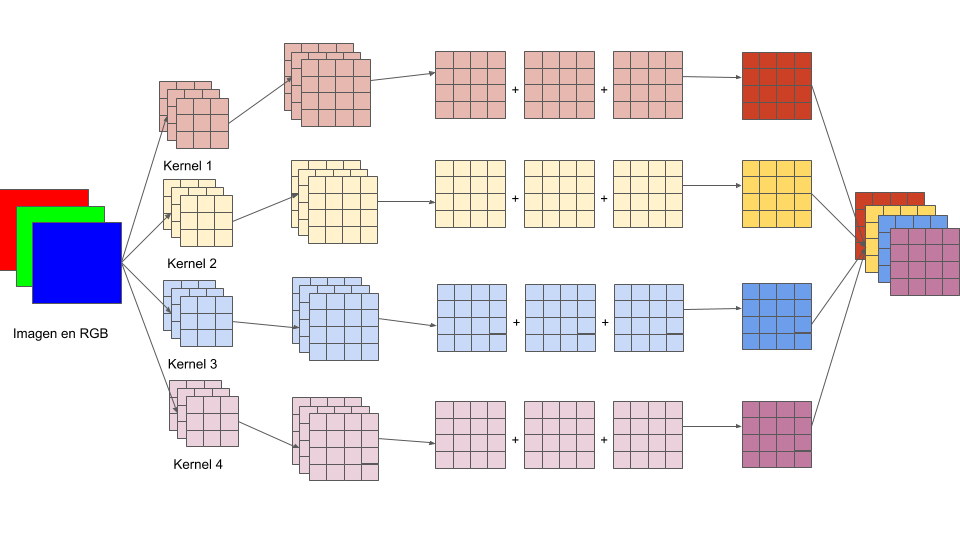
\includegraphics[width=16cm,keepaspectratio]{XX_Figures/Fig_Mapa_caracteristicas.png}
	\caption{\footnotesize Aplicación de filtros convolucionales 2D para obtener mapas de características}
	\label{fig:Fig_Mapa_caracteristicas}
\end{figure}

En la Figura \ref{fig:Fig_Mapa_caracteristicas} se puede observar un ejemplo de cómo se aplican los filtros convolucionales 2D con profundidad de canales. En el ejemplo se aplica una capa convolucional de 4 filtros; cada filtro tiene la misma profundidad que los mapas de características de entrada (imagen en RGB), cada filtro convolucional se aplica por separado para cada canal para así obtener en total 12 mapas de características (3 mapas por filtro convolucional), luego se suman los mapas de características obtenidos por los filtros y se obtiene un mapa de características por cada uno de los 4 kernels. El resultado (4 mapas de características) es nuestro conjunto de mapas de características obtenido al aplicar los cuatro filtros convolucionales.\\

\begin{figure}[th]
	\centering
	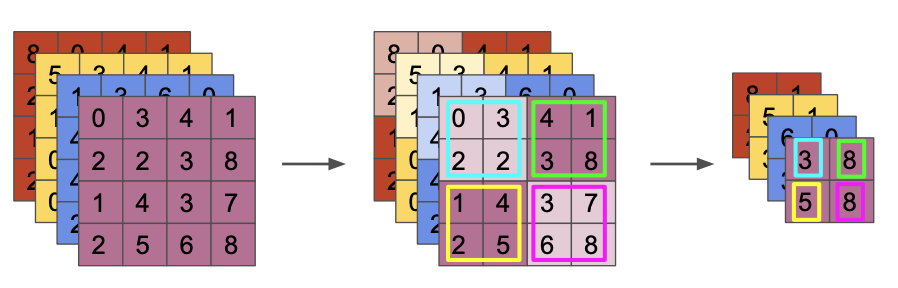
\includegraphics[width=14cm,keepaspectratio]{XX_Figures/Fig_Maxpooling.png}
	\caption{\footnotesize Aplicación de maxpooling de 2 x 2 a la salida mostrada en la Figura \ref{fig:Fig_Mapa_caracteristicas}}
	\label{fig:Fig_Maxpooling}
\end{figure}

La otra operación importante de las CNNs es la agrupación, (pooling) que asimila la labor que tienen las células complejas de la corteza visual de los mamíferos como se mencionó anteriormente. Las capas de agrupación (pooling layers) reducen la cantidad de parámetros que se tienen; esto se logra reduciendo dimensionalmente cada mapa de características obtenidos por nuestra capa convolucional. Hay diferentes capas de agrupación, pero la más usada es la MaxPooling Layer. Esta toma el elemento mas significativo de una ventana definida de nuestro mapa de características.\\

En la Figura \ref{fig:Fig_Maxpooling}, se observa la continuación del ejemplo de la Figura \ref{fig:Fig_Mapa_caracteristicas}, se le añadieron valores numéricos para poder explicar el funcionamiento de la operación maxpooling. Después de aplicar los 4 kernel convolucionales y obtener 4 mapas de características, se aplica un maxpooling de 2 x 2. El mapa de características delantero (morado), es dividido en ventanas de 2 x 2 y para cada una de las ventanas se obtiene el valor más grande. Esta operación se realiza para cada mapa de características. De esta manera se logra reducir el número de parámetros y obtener el valor más significativo de cada ventana en la que fueron divididos los mapas de características.

\begin{figure}[th]
	\centering
	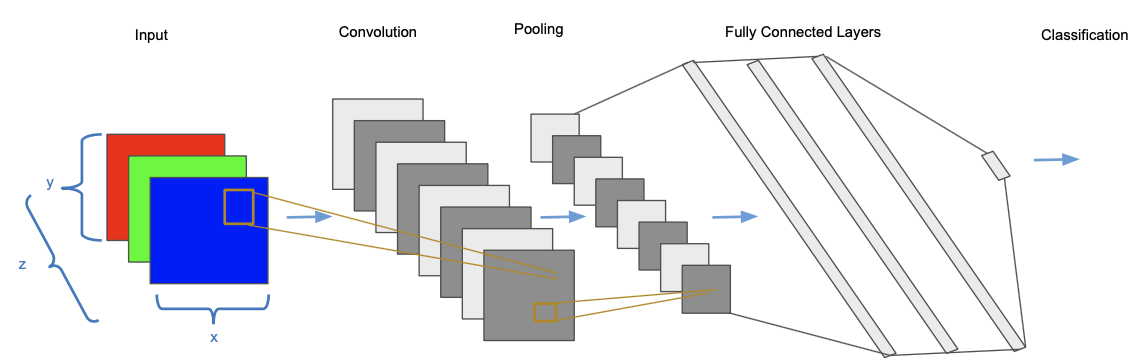
\includegraphics[width=16cm,keepaspectratio]{XX_Figures/Fig_CNN_Arquitecture.png}
	\caption{\footnotesize Arquitectura general de una CNN con una MLP profunda}
	\label{fig:Fig_CNN_Arquitecture}
\end{figure}

\begin{figure}[th]
	\centering
	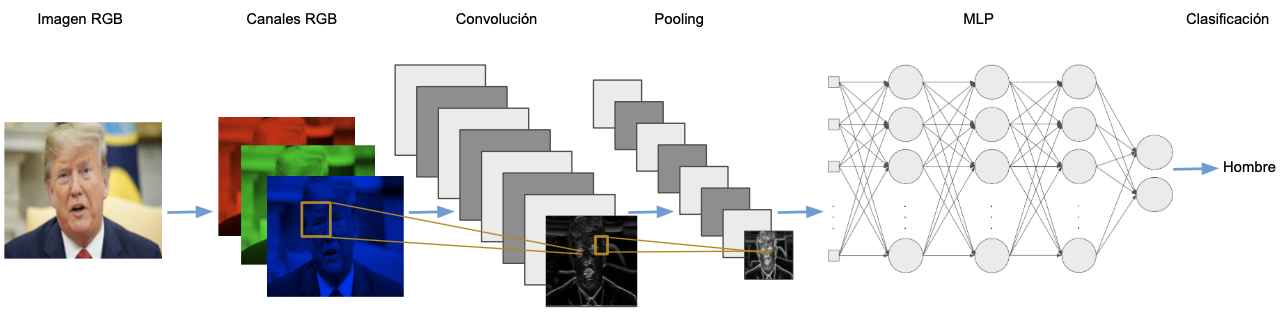
\includegraphics[width=17cm,keepaspectratio]{XX_Figures/Fig_CNN_Example.png}
	\caption{\footnotesize Ejemplo de la aplicación de una CNN con una MLP profunda}
	\label{fig:Fig_CNN_Example}
\end{figure}

Las CNNs son comúnmente utilizadas para extraer características en imágenes de una manera más práctica a comparación con las MLPs ya que requieren menos parámetros para la extracción automática de características en señales, imágenes o video. En la Figura \ref{fig:Fig_CNN_Arquitecture}, se muestra un esquema de cómo se utilizan las CNNs; se observa que una vez finalizada la extracción de características, se utiliza la salida de las CNNs como la entrada de la MLP encargada de igual forma de la extracción de más características y de la tarea de clasificación que se desea, como se muestra en el ejemplo de la Figura \ref{fig:Fig_CNN_Example}.

%----------------------------------------------------------------------------------------
\subsubsection{3D CNN}
\label{3DCNN}
%----------------------------------------------------------------------------------------

Este tipo de arquitectura de red convolucional se aplica cuando se requieren obtener características espaciales (como en la Figura \ref{fig:Fig_CNN_Example}) y características temporales.\\

\begin{figure}[p]
	\centering
	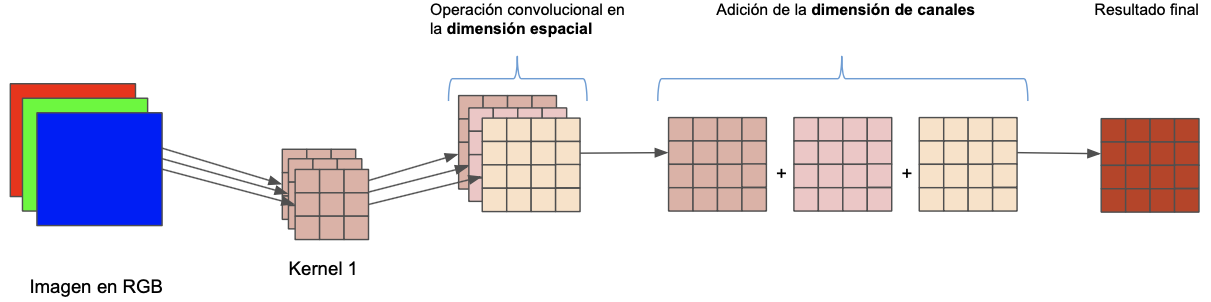
\includegraphics[width=13cm,keepaspectratio]{XX_Figures/Fig_2D_Dimensiones.png}
	\caption{\footnotesize Dimensiones y operaciones de una 2D CNN con un kernel}
	\label{fig:Fig_2D_Dimensiones}
\end{figure}

\begin{figure}[p]
	\centering
	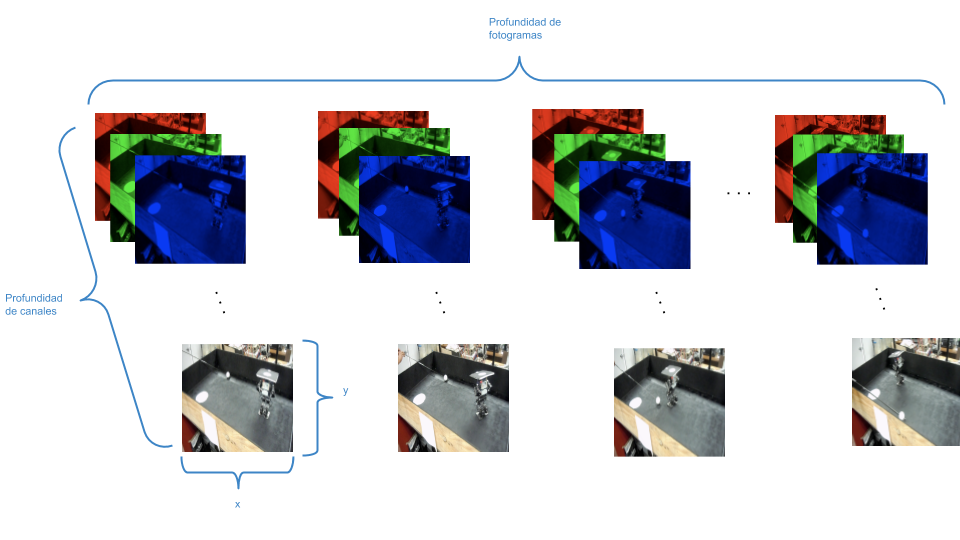
\includegraphics[width=13cm,keepaspectratio]{XX_Figures/Fig_Video.png}
	\caption{\footnotesize Las 4 dimensiones que posee un video}
	\label{fig:Fig_Video}
\end{figure}

\begin{figure}[p]
	\centering
	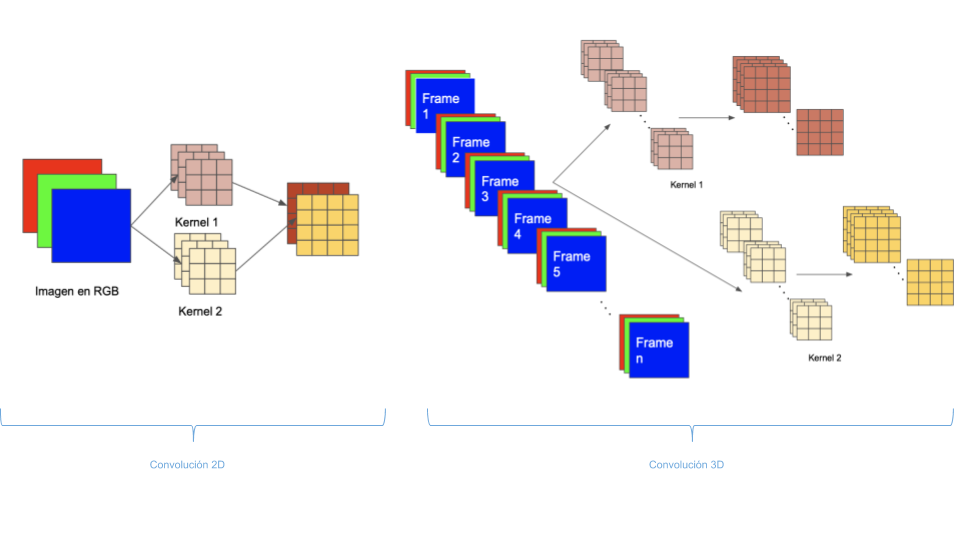
\includegraphics[width=13cm,keepaspectratio]{XX_Figures/Fig_CNN_2Dvs3D.png}
	\caption{\footnotesize Diferencias entre una convolución 2D y 3D}
	\label{fig:Fig_CNN_2Dvs3D}
\end{figure}

\begin{figure}[p]
	\centering
	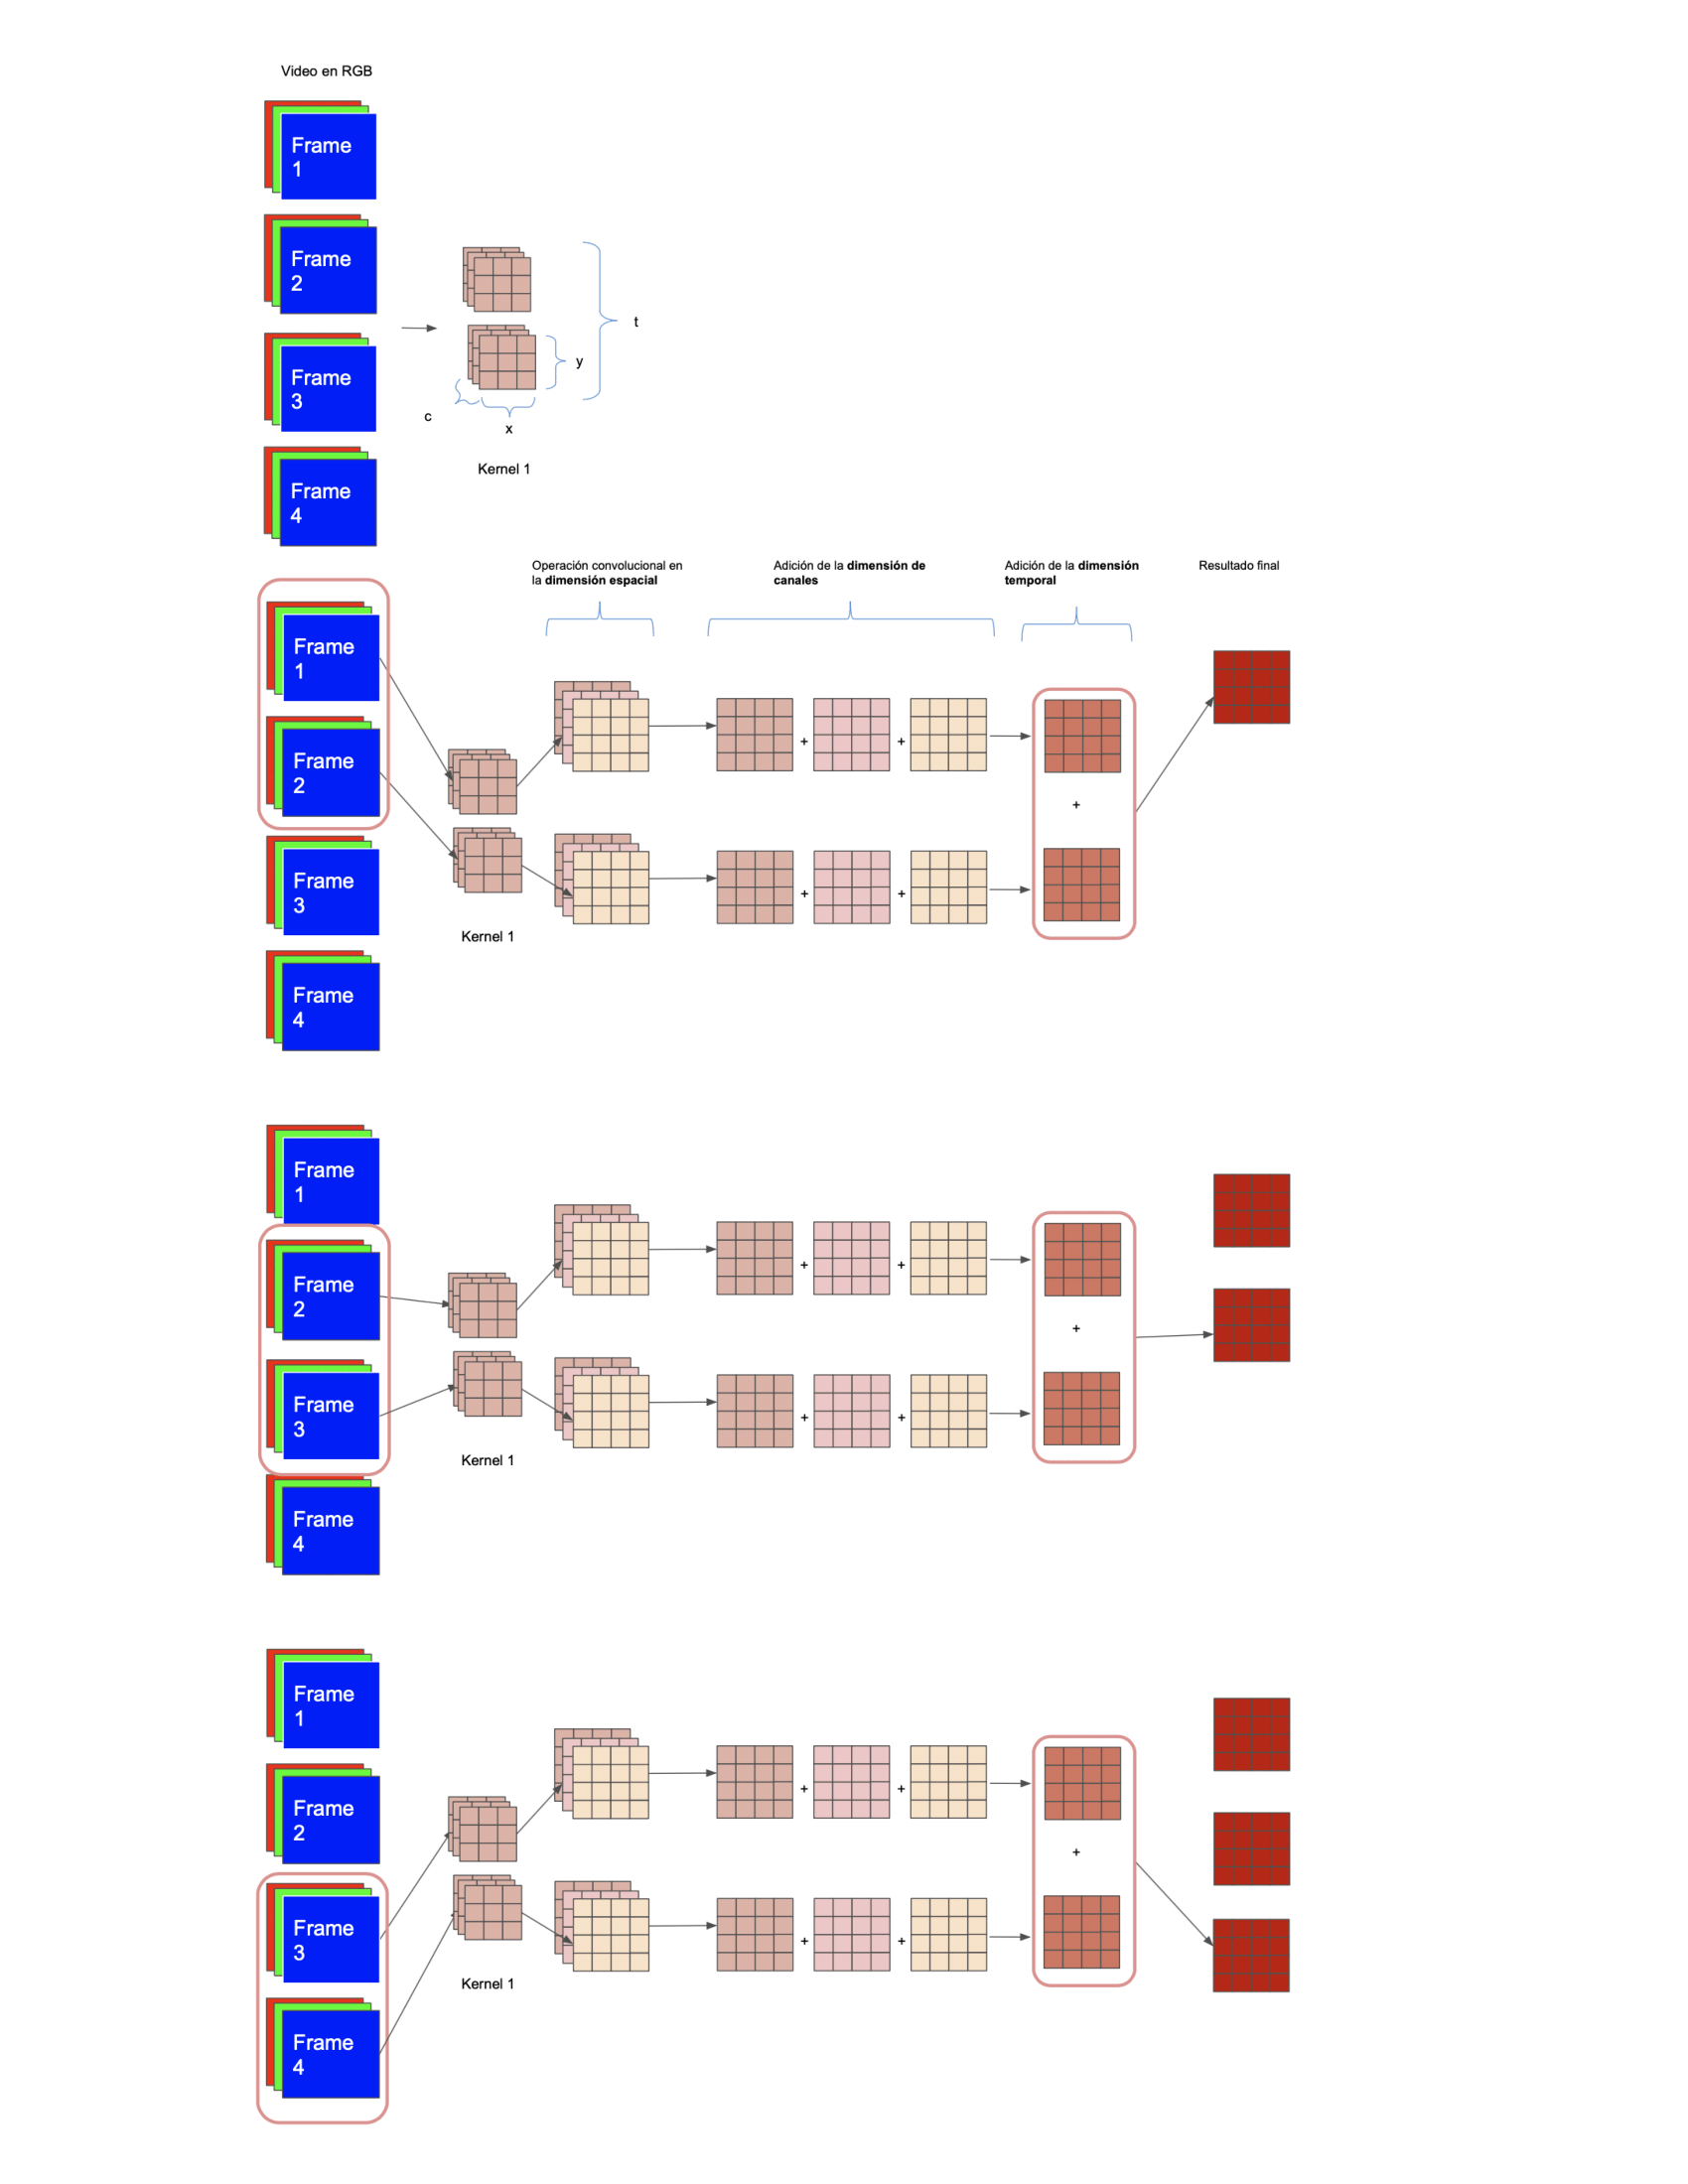
\includegraphics[width=18cm,keepaspectratio]{XX_Figures/Fig_Ejemplo_3DCNN.png}
	\caption{\footnotesize Ejemplo de los pasos en una 3D CNN con un kernel}
	\label{fig:Fig_Ejemplo_3DCNN}
\end{figure}

\begin{figure}[p]
	\centering
	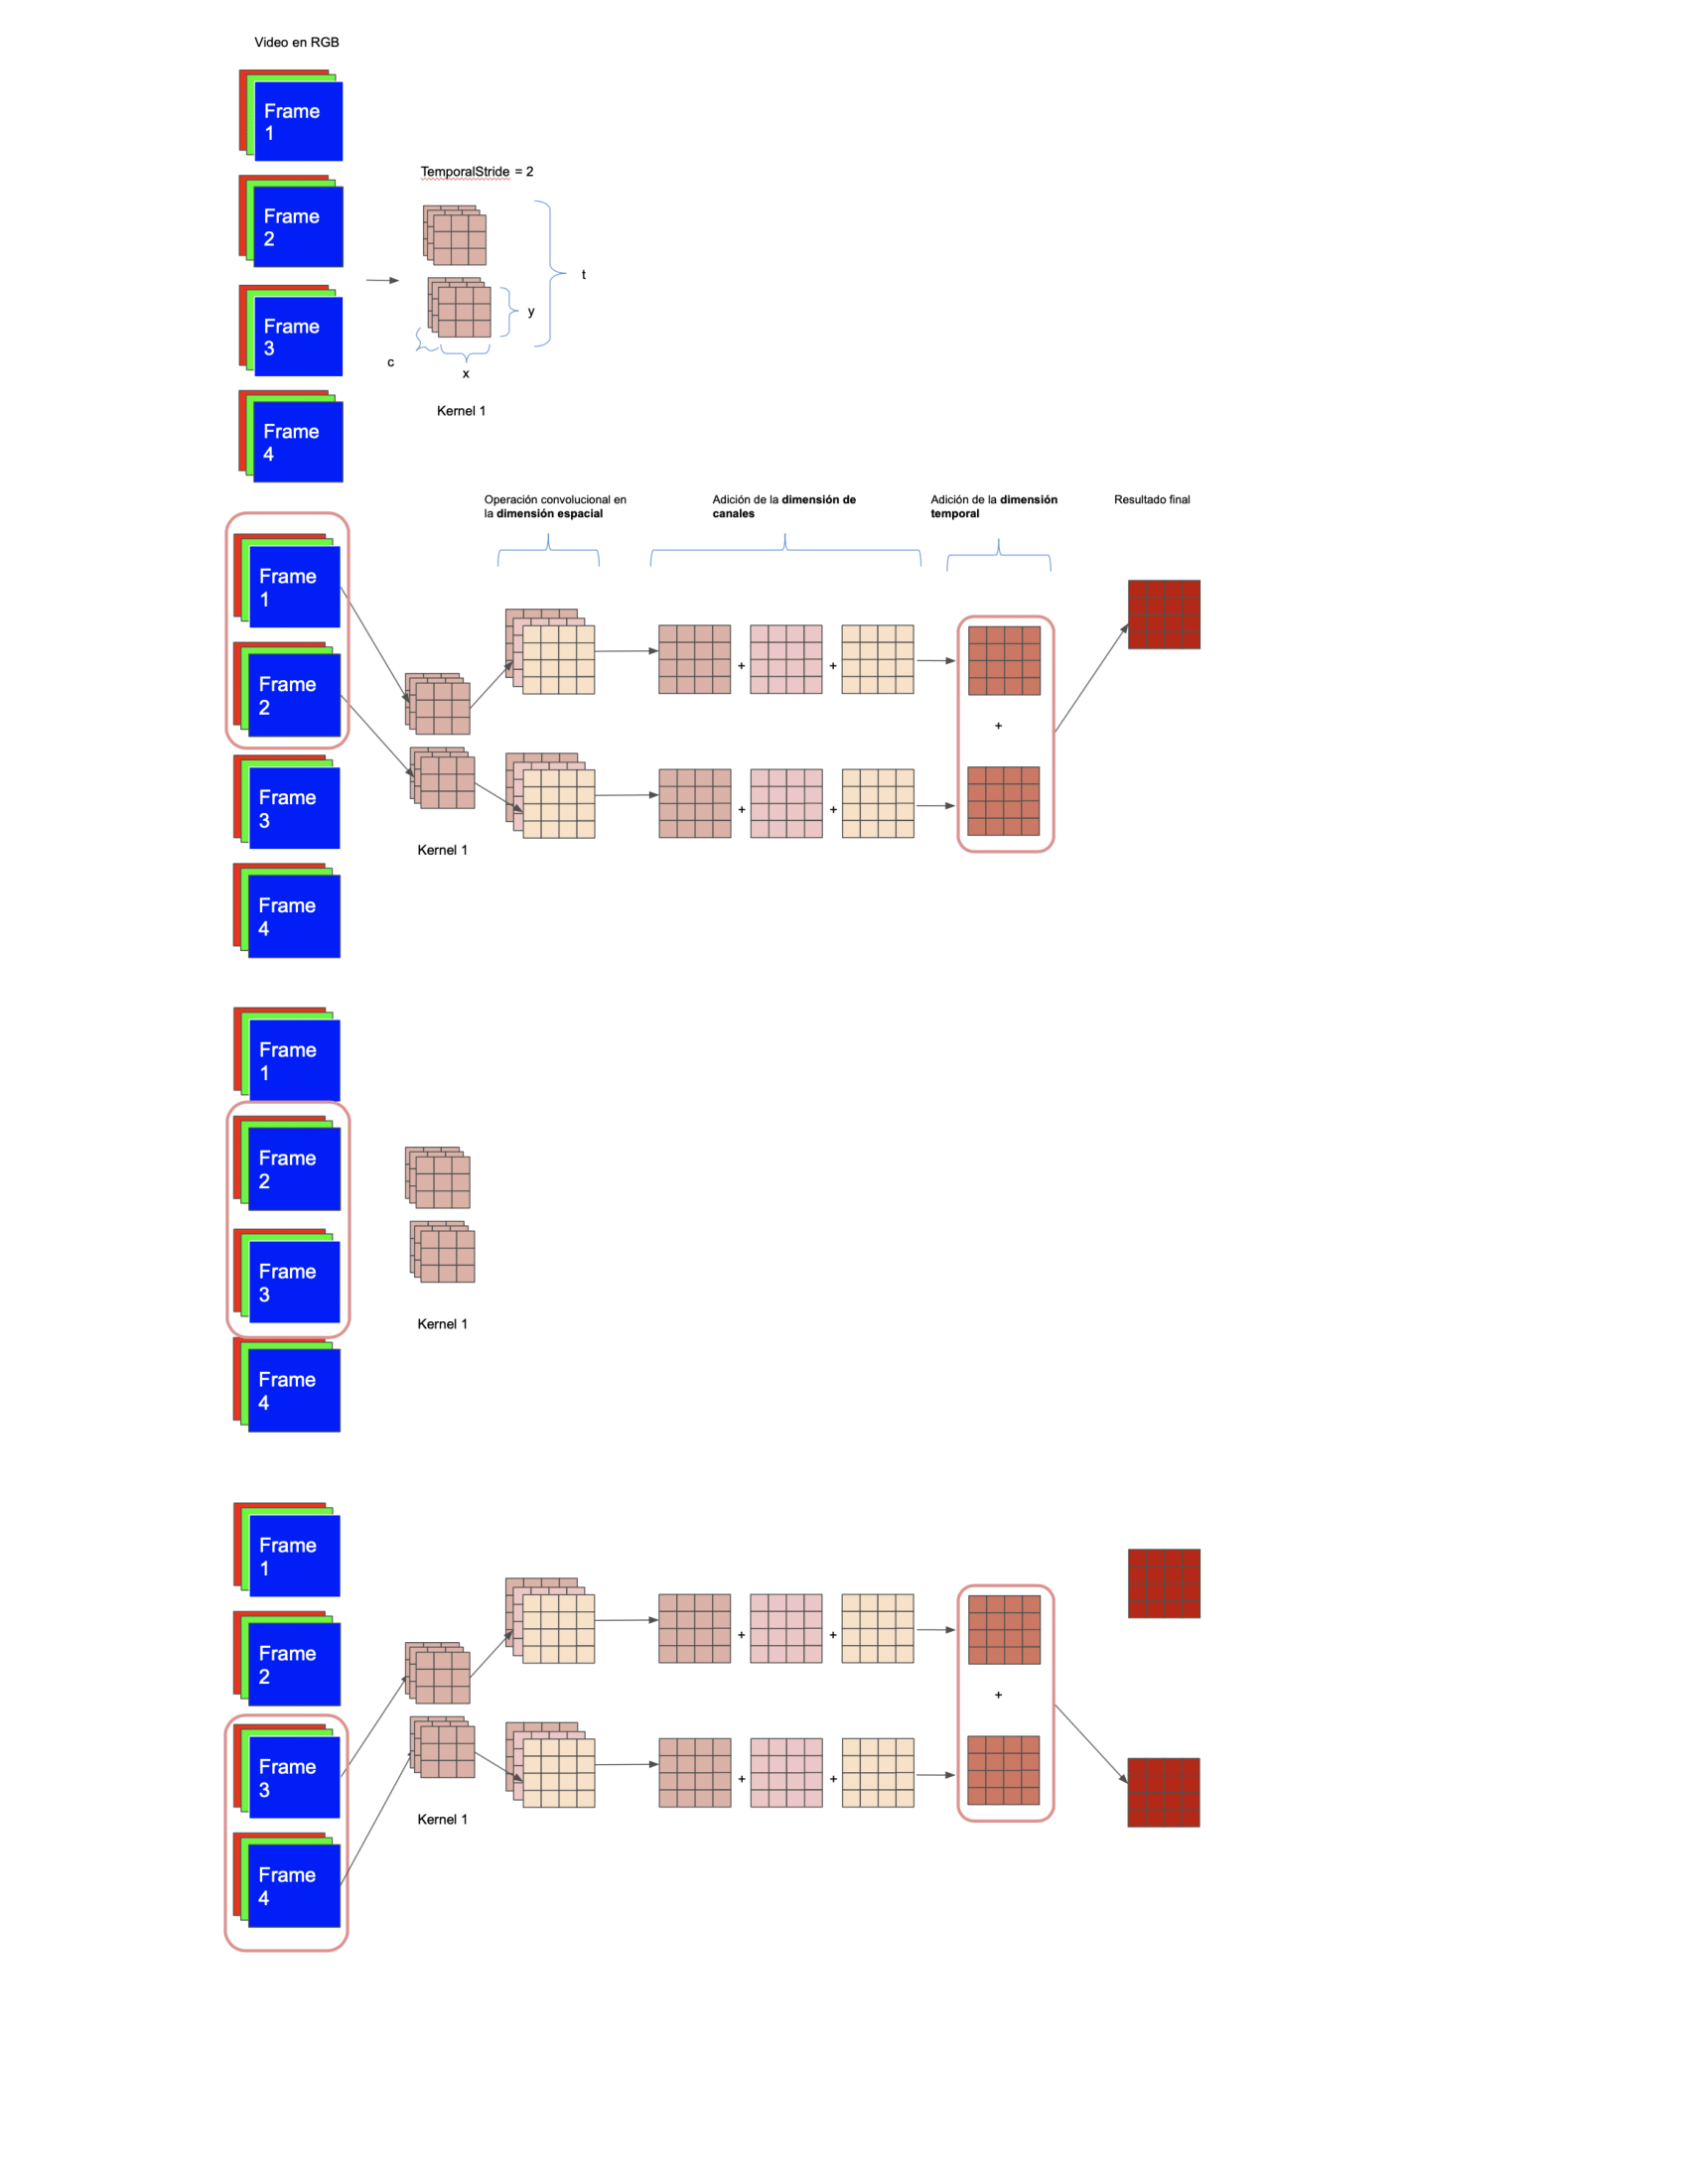
\includegraphics[width=19cm,keepaspectratio]{XX_Figures/Fig_3DCNN_TemporalStride.png}
	\caption{\footnotesize Ejemplo de la Figura \ref{fig:Fig_Ejemplo_3DCNN} con TemporalStride = 2}
	\label{fig:Fig_3DCNN_TemporalStride}
\end{figure}

Se ha demostrado que varias arquitecturas de red 3D CNN son capaces de extraer características espaciotemporales capturando la información del movimiento en de los fotogramas adyacentes en un video \cite{Ji20133DRecognition}. Las redes 2D CNNs previamente analizadas están enfocadas generalmente en analizar imágenes las cuales están en 2 dimensiones (una matriz); aunque estrictamente se encuentran en 3 dimensiones por la profundidad de los canales que pueden llegar a tener, pero comúnmente en la literatura las mencionan como redes neuronales convolucionales 2D por las dos operaciones que se hacen para llegar al resultado final como se observa en la figura \ref{fig:Fig_2D_Dimensiones}. Se agrega una dimensión extra a las redes neuronales convolucionales 3D, esta es la dimensión temporal que en un video representa los diferentes fotogramas que tiene. Un ejemplo de esta nueva dimensión se puede apreciar en el ejemplo de la Figura \ref{fig:Fig_Video}\\


En la Figura \ref{fig:Fig_CNN_2Dvs3D} se puede observar las diferencias entre una 2D CNN y una 3D CNN. En el caso de las 3D CNN los kernels tienen una anchura y una altura que es la encargada de aplicar la operación convolucional a la matriz de píxeles (dimensión espacial) de la misma manera que lo hace una 2D CNN; tiene una profundidad que es igual a la la dimensión de los canales que tienen nuestras matrices (por lo general tres canales: RGB) y se hace la misma operación de adición de la dimensión de canales que en las 2D CNN como se muestra en la Figura \ref{fig:Fig_2D_Dimensiones}. La siguiente dimensión que tienen los kernels en la 3D CNN es la dimensión temporal que como se nota en la Figura \ref{fig:Fig_CNN_2Dvs3D} en la que parecería que cada kernel de la 3D CNN  tiene varios kernels; esta nueva dimensión es la encargada de tomar los datos de varios fotogramas (frames) en los videos y juntarlos en una sola matriz de características.\\ 

En la Figura \ref{fig:Fig_2D_Dimensiones} se muestran las operaciones dimensionales que una 2D CNN hace cuando se tiene un kernel y una imagen con tres canales RGB. Se observa en la Figura \ref{fig:Fig_Ejemplo_3DCNN} las operaciones que hace una red 3D CNN con los mismos hiperparámetros que la 2D CNN de la Figura \ref{fig:Fig_2D_Dimensiones} (un kernel e imágenes en RGB) pero con la diferencia de que se aplican las convoluciones a un video con 4 fotogramas (frames). En el primera parte de la Figura \ref{fig:Fig_Ejemplo_3DCNN} se observan los 4 fotogramas con sus 3 canales respectivos y un kernel con dimensión \textit{(t,c,y,x)} en la que \textit{(y,x) = (3,3)} corresponden al plano espacial, \textit{c = 3} corresponde a la dimensión de los canales (RGB) y \textit{t = 2} corresponde a la dimensión temporal que tiene el kernel. Como la entrada es una cierta cantidad de fotogramas, entonces \textit{t = 2} indica que se aplicará el filtro convolucional a dos fotogramas. En la segunda parte de la \ref{fig:Fig_Ejemplo_3DCNN} se observa que la convolución se aplica para los dos primeros fotogramas (fotograma 1 y fotograma 2) por separado. Se aplica el kernel 1 con el primer fragmento para el fotograma uno y se hace la misma operación convolucional y de adición de las dimensiones de canales que en la 2D CNN; después se aplica el kernel 1 con el segundo fragmento del kernel convolucional y se hace el mismo procedimiento; el resultado de los dos fragmentos del kernel 1 hacen una adición de las matrices resultantes correspondientes al plano temporal y termina el primer paso de la convolución. El segundo paso consiste en deslizar una posición hacia abajo el kernel 3D. Durante en transcurso de este trabajo nos referiremos al deslizamiento temporal como TemporalStride. Una vez aplicado el TemporalStride una posición, se vuelve a aplicar el kernel 1 para el fotograma 2 y fotograma 3, y se vuelva a hacer el mismo procedimiento que en el primer paso para obtener una matriz con características conjuntas del fotograma 2 y 3. Para el último paso se vuelve a aplicar un TemporalStride en una posición y se hace el mismo procedimiento que en los dos pasos anteriores. Al final se habrá obtenido 3 matrices de características que contienen información conjuntas de los 4 fotogramas de entrada y termina la operación convolucional 3D. \\

Las redes convolucionales 3D contienen los mismos atributos que las redes convolucionales 2D, tales como el Stride, Padding (mostrados en el Capítulo \ref{Filtros_espaciales}), la operación Pooling y un Kernel \textit{k = (c,y,x)}, pero a diferencia con las 2D CNN, las 3D CNN contienen un kernel de dimensión \textit{k = (t,c,y,x)}. También contienen un nuevo hiperparámetro el cuál es el paso temporal (TemporalStride) que indica cuántas posiciones en la dimensión temporal se desea que se mueva el kernel. Un ejemplo se observa en la Figura \ref{fig:Fig_3DCNN_TemporalStride} el cuál toma como referencia el ejemplo de la Figura \ref{fig:Fig_Ejemplo_3DCNN} pero con \textit{TemporalStride = 2}.//

La habilidad de analizar series de fotogramas o imágenes en algún contexto le ha dado a las convoluciones 3D varios usos como por ejemplo reconocimiento de acciones \cite{Yang2017DeepImages}; a través de secuencias de imágenes 2D se puede lograr interpretar el movimiento de los objetos para poder predecir ciertas situaciones. También a través del reconocimiento de acciones humanas se ha podido clasificar  los diferentes movimientos que hace un ser humano y con qué objetivo; esto ha sido de gran utilidad para tecnologías que asisten a los humanos, sistemas de seguridad y aplicaciones de realidad virtual. Otro ejemplo en la cual es usada la red 3D CNN es la evaluación de imágenes médicas; estas imágenes se realizan mediante la captura de cortes de la profundidad del tejido a evaluar, combinando estas imágenes estáticas, se ha logrado la identificación de células cancerosas y la evaluación de la salud arterial \cite{Ji20133DRecognition}.\\

El trabajo actual esta enfocado en analizar videos, por lo tanto el uso de la red convolucional 3D es una excelente propuesta para la extracción de características espaciotemporales.

\begin{figure}[th]
	\centering
	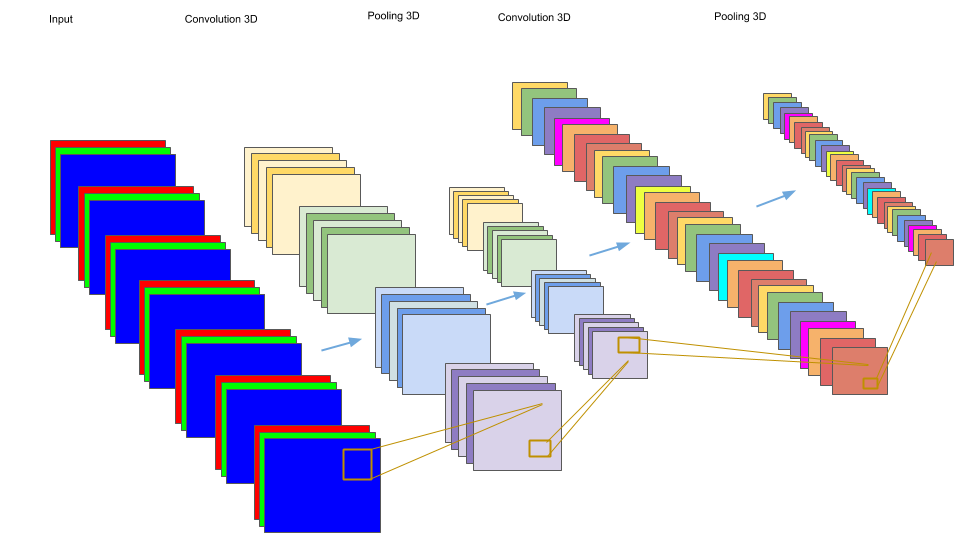
\includegraphics[width=17cm,keepaspectratio]{XX_Figures/Fig_3DCNN_Esquema.png}
	\caption{\footnotesize Esquema de una 3D CNN}
	\label{fig:Fig_3DCNN_Esquema}
\end{figure}

En la Figura \ref{fig:Fig_3DCNN_Esquema}, se muestra un esquema general de las redes neuronales 3D utilizadas para extraer características en videos RGB.


\end{onehalfspacing}
		
		%INCLUIR EL CAPÍTULO 3
		% Chapter 3
%----------------------------------------------------------------------------------------
\chapter{Estado del Arte} % Main chapter title
\label{Chapter3} % For referencing the chapter elsewhere, use \ref{Chapter3} 
\begin{onehalfspacing}

Este capítulo presenta las pruebas que han hecho diferentes estudios y sus resultados. A pesar de que el detectar si una persona es veraz o falsa en sus declaraciones ha sido una investigación bastante estudiada y antigua. Siguen realizando diferentes estudios y metodologías para encontrar los verdaderos rasgos que dan indicio a una verdad y a una mentira, esto con el fin de poder generalizar la tarea de clasificar verdades o mentiras.\\


David Raskin y Gunter Kohnken, especialistas en detección de mentiras, creen que detectar mentiras a través de pistas no verbales es una metodología en la que la gente no puede confiar. Detectar mentiras a través del lenguaje no verbal tiene una exactitud (porcentaje de respuestas correctas) entre el 45 y 60\%. Las personas tienen una exactitud para detectar verdades del 67\% y 44\% para detectar mentiras \cite{Vrij2000DetectingBehavior,Bond2006AccuracyJudgments}.\\

Vrij en el año 2000 \cite{Vrij2000DetectingBehavior} examinó en su trabajo la hipótesis de que a través de un análisis sistemático del comportamiento no verbal podía ser capaz de detectar mentiras y verdades en un individuo. Analizaron el lenguaje no verbal a través de dos personas que observaron y anotaron el comportamiento de videos en donde aparecían varias personas mintiendo y diciendo verdades, analizando las veces en el cual una persona desvía la mirada, sonríe, mueve los pies, mueve los dedos, etc. Obtuvieron un 78\% de exactitud en la clasificación de mentiras y verdades, mientras que un grupo de estudiantes que intentaron detectar mentiras con el mismo conjunto de datos obtuvo un accuracy del 53\%. \\ 


\begin{table}[h!]
\centering
    \begin{tabular}{|c|c|c|}
        \hline 
        feature Set & DT & RF\tabularnewline
        \hline 
        \hline 
        Unigrams & 60.33\% & 56.19\%\tabularnewline
        Bigrams & 52.71\% & 51.20\%\tabularnewline
        Facial displays & 70.24\% & 76.03\%\tabularnewline
        Hand gestures & 61.98\% & 62.80\%\tabularnewline
        Uni + Facial displays & 66.94\% & 57.02\%\tabularnewline
        \hline 
        All verbal & 60.33\% & 50.41\%\tabularnewline
        All non-verbal & 68.59\% & 73.55\%\tabularnewline
        \hline 
        All features & 75.20\% & 50.41\%\tabularnewline
        \hline 
    \end{tabular}%
	\caption{Resultados del trabajo de Verónica en el 2015}
	\label{tab:Fig_Veronica2015}
\end{table}

\begin{table}[h!]
\centering
    \begin{tabular}{|c|c|c|c|c|}
        \cline{2-5} \cline{3-5} \cline{4-5} \cline{5-5} 
        \multicolumn{1}{c|}{} & Text & Audio & Silent video & Full video\tabularnewline
        \hline 
        A1 & 54.55\% & 51.24\% & 45.30\% & 56.20\%\tabularnewline
        \hline 
        A2 & 47.93\% & 55.37\% & 46.28\% & 53.72\%\tabularnewline
        \hline 
        A2 & 50.41\% & 59.50\% & 47.93\% & 59.50\%\tabularnewline
        \hline 
        Sys & 60.33\% & NA & 68.59\% & 75.20\%\tabularnewline
        \hline 
    \end{tabular}%
	\caption{Resultados obtenidos de tres diferentes personas presentados en el trabajo de Verónica en el 2015}
	\label{tab:Fig_Veronica2015anotadores}
\end{table}

En el 2015 Verónica Pérez junto con su equipo de la Universidad de Michigan desarrollaron un sistema multimodal combinando modalidades verbales y no verbales para detectar mentiras en un conjunto de datos que recopilaron y etiquetaron; este conjunto de datos contiene videos de juicios de cortes de Estados Unidos en la cuál aparecen diferentes personas dando declaraciones falsas y verdaderas. Obtuvieron una exactitud en su clasificación en un rango de 60-75\%, con un modelo que extrae y combina características lingüísticas y gestos.  Ellos anotaron los gestos observados en los videos usando una metodología justificada y probada, dándole más prioridad al rostro y a los movimientos de la mano. Crearon un vector combinando características verbales y no verbales y dos algoritmos clasificadores; el primero utilizando Decision Trees (DT) y Random Forest (RF) utilizando leave one out cross validation. Obtuvieron una exactitud de 75.20\% al utilizar DT  y combinando todas las características verbales y no verbales; en características no verbales obtuvieron un 68.59\% de exactitud con DT y 73.55 de exactitud con RF.  En la Tabla \ref{tab:Fig_Veronica2015} se observa la exactitud que obtuvieron sus dos propuestas y en la tabla \ref{tab:Fig_Veronica2015anotadores} la exactitud que obtuvieron 3 anotadores \cite{Perez-Rosas2015VerbalDetection}.\\

\begin{table}[h!]
\centering
    \begin{tabular}{|c|c|c|}
        \hline 
        Feature Set & Interview & Trials\tabularnewline
        \hline 
        \hline 
        Baseline & 54.83\% & 55.35\%\tabularnewline
        \hline 
        Unigrams & 70.80\% & 82.14\%\tabularnewline
        \hline 
        Psycholinguistics & 59.67\% & 50.50\%\tabularnewline
        \hline 
        Syntactic Complexity & 54.83\% & 60.71\%\tabularnewline
        \hline 
        Facial Displays & 70.96\% & 80.35\%\tabularnewline
        \hline 
        Hand Gestures & 56.45\% & 48.21\%\tabularnewline
        \hline 
        Unigr. + Facial Disp. & 70.96\% & 76.78\%\tabularnewline
        \hline 
        All Verbal & 70.96\% & 64.28\%\tabularnewline
        \hline 
        All Nonverbal & 67.14\% & 83.92\%\tabularnewline
        \hline 
        All features & 79.03\% & 82.14\%\tabularnewline
        \hline 
    \end{tabular}%
    \caption{\footnotesize Resultados del trabajo de Verónica con dos datasets utilizando SVM}
	\label{tab:Fig_Veronica2datasets}
\end{table}

\begin{table}[h!]
\centering
    \begin{tabular}{|c|c|c|}
        \hline 
        Training & Test & SVM\tabularnewline
        \hline 
        \hline 
        Trials & Interviews & 58.06\%\tabularnewline
        \hline 
        Interview & Trials & 58.92\%\tabularnewline
        \hline 
    \end{tabular}%
	\caption{\footnotesize Resultados del trabajo de Verónica entrenando su SVM con un dataset y haciendo pruebas con el segundo dataset}
	\label{tab:Fig_VeronicaCrossDomain}
\end{table}

Verónica en septiembre del año 2015 volvió a probar el sistema con otro conjunto de datos y los resultados que obtuvo se presentan en la Figura \ref{tab:Fig_Veronica2datasets}, en donde se puede observar que su sistema multimodal alcanzó un accuracy del 82.14\% en el dataset `Trial' (conjunto de datos que habían ocupado previamente \ref{tab:Fig_Veronica2015}) y una exactitud de 79.03\% en el nuevo conjunto de datos `Interview' utilizando SVM como clasificador. Pero se dieron cuenta que al entrenar su clasificador con el dataset `Trial' y hacer las pruebas con el dataset `Interview', la exactitud de su modelo bajaba considerablemente, llegando a la conclusión de que el el rendimiento de su sistema bajaba considerablemente si no existía una superposición entre los datos del entrenamiento y los datos de prueba. Los resultados de su modelo con el entrenamiento de un dataset y las pruebas con el segundo dataset se observan en la Figura \ref{tab:Fig_VeronicaCrossDomain}.\\

\begin{table}[h!]
\centering
    \begin{tabular}{|c|c|c|c|c|c|c|c|}
        \hline 
        Features & L-SVM & K-SVM & NB & DT & RF & LR & Adaboost\tabularnewline
        \hline 
        \hline 
        IDT & 0.7731 & 0.6374 & 0.5984 & 0.5895 & 0.5567 & 0.6425 & 0.6591\tabularnewline
        \hline 
        MicroExpression & 0.7502 & 0.7540 & 0.7629 & 0.7269 & 0.8064 & 0.7398 & 0.7507\tabularnewline
        \hline 
        Transcript & 0.6457 & 0.4667 & 0.6625 & 0.5251 & 0.6172 & 0.5643 & 0.6416\tabularnewline
        \hline 
        MFCC & 0.7694 & 0.8171 & 0.6726 & 0.4369 & 0.7393 & 0.6683 & 0.6900\tabularnewline
        \hline 
        IDT+MicroExpression & 0.8347 & 0.7540 & 0.7629 & 0.7687 & 0.8184 & 0.7419 & 0.7507\tabularnewline
        \hline 
        IDT-MicroExpression+Transcripts & 0.8347 & 0.7540 & 0.7776 & 0.7777 & 0.8184 & 0.7419 & 0.7507\tabularnewline
        \hline 
        IDT+MicroExpression+MFCC & 0.8596 & 0.8233 & 0.7629 & 0.7687 & 0.8477 & 0.7894 & 0.7899\tabularnewline
        \hline 
        All Modalities & 0.8773 & 0.8233 & 0.7776 & 0.7777 & 0.8477 & 0.7894 & 0.7899\tabularnewline
        \hline 
    \end{tabular}
	\caption{\footnotesize Resultados del trabajo de Wu}
	\label{tab:Fig_Wu_2017}
\end{table}


En el año 2018 Zhe Wu presentó un sistema para detectar mentiras de manera automática en videos del dataset creado por Verónica (Trial). Extrayendo características visuales a través de la trayectoria densa mejorada (IDT) la cuál ha sido utilizada anteriormente para reconocer acciones, resultó tener un resultado positivo para predecir mentiras en videos. Obtuvieron un AUC (Area debajo de la curva precision-recall) de 0.877 cuando evaluaron su sistema con sujetos que no eran parte del conjunto de entrenamiento. Utilizaron un modelo multimodal en la que también incluyeron anotaciones humanas de las micro expresiones en los videos obteniendo un AUC de 0.922. Tuvieron la necesidad diferentes tipos de software que fueran capaz de obtener microexpresiones y de múltiples características verbales y no verbales. En la Tabla \ref{tab:Fig_Wu_2017}, se muestran los resultados obtenidos utilizando diferentes características y clasificadores.\\

\begin{equation}
        d_{i4} - D 
    \begin{cases}
        > 0,& \text{subject  } i \ = D\\
        \le 0,& \text{subject } i \ = ND\\
    \end{cases}
    \label{fig:Figura_Tsiamyrtzis}
\end{equation}

Tsiamyrtzis en el año 2005 hizo un detector de mentiras a través de señales que indican el promedio de temperatura periorbital en el rostro de una persona, por cada frame de temperatura que procesaron, ocuparon el promedio del 10\% de los píxeles con mayor temperatura y utilizaron un método de reconocimiento de patrones para clasificar como sujeto estresado (Mentira) y no-estresado (No mentira) Obtuvieron una tasa de clasificación del 87.2\% para 39 sujetos.
Calcularon una pendiente \textit{$D_{i}$} de la señal de la temperatura filtrada que corresponden a la duración completa del interrogatorio para cada sujeto i y calcularon la pendiente \textit{$d_{i4}$} de la porción de la señal que corresponde a la sesión de preguntas y respuestas con el factor de impacto más alto (nivel de estrés psicológico percibido que tiene una pregunta por unidad de tiempo). En otras palabras, para que una pregunta tenga un factor de alto impacto, no solo es necesario ser "duro" sino también breve. La toma de decisiones se hacía a través de la comparación de la ecuación \ref{fig:Figura_Tsiamyrtzis}
\cite{Tsiamyrtzis2005LieVideo}.\\

En el año 2010 Lara Warmelink desarrolló junto con su equipo, una herramienta capaz de detectar mentiras a través de imágenes térmicas. La prueba consistió 51 pasajeros en un aeropuerto internacional en la que tenían que mentir o decir la verdad acerca de su próximo viaje en una entrevista. La temperatura emanada por su piel fue grabada a través de una cámara térmica; los mentirosos tenían una temperatura más alta que los que decían la verdad. Obtuvieron 64\% para clasificar a los sujetos mentirosos y 69\% para clasificar a los sujetos veraces \cite{Warmelink2011ThermalAirports}.\\

Bashar A. Rajoub en Junio del 2014 a través de el método K vecinos más cercanos (k-nearest neighbors) que es un método de clasificación supervisada, logró clasificar 492 respuestas térmicas) utilizando diferentes estrategias para representar los datos y reportó una habilidad para predecir mentiras y verdades del 58\% a través de \textit{leave-one-person-out} y de 86.88\% con \textit{within-indidivual}. La metodología \textit{leave-one-person-out} básicamente lo que hace es que separa a un sujeto del conjunto de entrenamiento y todos los demás sujetos son utilizados par entrenar el sistema. El pobre desempeño predictivo que tuvieron con esta metodología se debe al hecho de que la distribución conjunta de probabilidad de las entradas (datos térmicos) y las salidas (etiquetas de clase) de la persona de prueba era diferente a la distribución conjunta formada por todas las demás personas en el conjunto de entrenamiento. En cambio cuando con la metodología \textit{within-indidivual} no sucedía esto porque separaban n-1 datos de un sujeto para el entrenamiento y el sobrante para las pruebas de su sistema; de esta manera obtuvieron hasta un 86.88\% \cite{Rajoub2014ThermalDetection}.\\

Desafortunadamente la mayoría de los trabajos que utilizaron cámaras térmicas se vieron en la necesidad de calibrar las cámaras y tener un escenario completamente controlado. De igual forma las cámaras que se ocuparon son de un costo mayor a los \$1000 USD
\begin{figure}[h!]
	\centering
	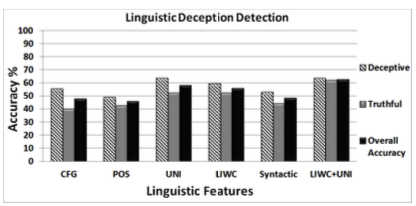
\includegraphics[width=7cm,keepaspectratio]{XX_Figures/Fig_Veronica_Linguistic.png}
	\caption{\footnotesize Accuracy obtenido por Aboulenien utilizando diferentes conjuntos de características linguisticas. \cite{Abouelenien2016AnalyzingApproach} .}
	\label{fig:Fig_Veronica_Linguistic}
\end{figure}

\begin{figure}[h!]
	\centering
	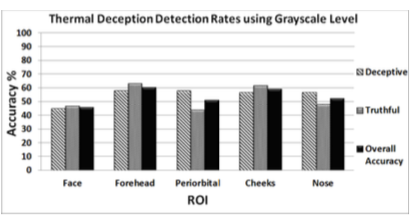
\includegraphics[width=7cm,keepaspectratio]{XX_Figures/Fig_Veronica_Termico_GS.png}
	\caption{\footnotesize Accuracy obtenido por Aboulenien utilizando características térmicas en escala de grises. \cite{Abouelenien2016AnalyzingApproach}.}
	\label{fig:Fig_Veronica_Termico_GS}
\end{figure}

\begin{figure}[h!]
	\centering
	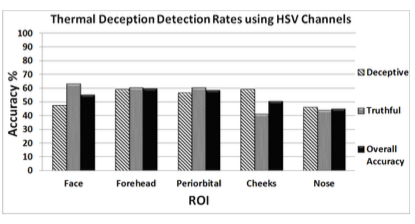
\includegraphics[width=7cm,keepaspectratio]{XX_Figures/Fig_Veronica_Termico_HSV.png}
	\caption{\footnotesize Accuracy obtenido por Aboulenien utilizando características térmicas en HSV. \cite{Abouelenien2016AnalyzingApproach}.}
	\label{fig:Fig_Veronica_Termico_HSV}
\end{figure}

En el año 2016, Verónica junto con un nuevo equipo creó un sistema  multimodal para detectar mentiras en la que integran características psicológicas, lingüísticas y térmicas basado en árboles de decisión, con el objetivo de crear un sistema completamente automático para detectar mentiras, de manera no invasiva y factible. En la Figura \ref{fig:Fig_Veronica_Linguistic}, se observan los resultados obtenidos a través de de 6 diferentes conjuntos de características, obteniendo una exactitud máximo de 62\% \cite{Abouelenien2016AnalyzingApproach}. Los resultados obtenidos extrayendo características térmicas en escala de grises se observan en la Figura \ref{fig:Fig_Veronica_Termico_GS} y en HSV en la Figura \ref{fig:Fig_Veronica_Termico_HSV}.\\

Krishnamurthy en el año 2018, creó un red neuronal multimodal capaz de detectar mentiras. Combinando características de video, audio, texto y micro-expresiones obtuvo hasta una exactitud del 96.14\%. Los diferentes modelos que utilizaron se muestran en la Figura \ref{fig:Figura_Navonil_Modelo}. De igual forma que Zhe Wu, realizaron las pruebas con individuos que pertenecen a un sistema nunca antes había visto (mismos sujetos no están en el conjunto de entrenamiento y conjunto de pruebas). Probaron el desempeño de su sistema por separado y con todas las modalidades. En la Tabla \ref{tab:Figura_Navonil_accuracy}, se puede observar que el modelo en el que solamente extraían características de los videos a través de una red 3D-CNN, obtenía una mayor exactitud que cualquier otro conjunto de características \cite{KrishnamurthyADetection}.\\

\begin{figure}[h!]
	\centering
	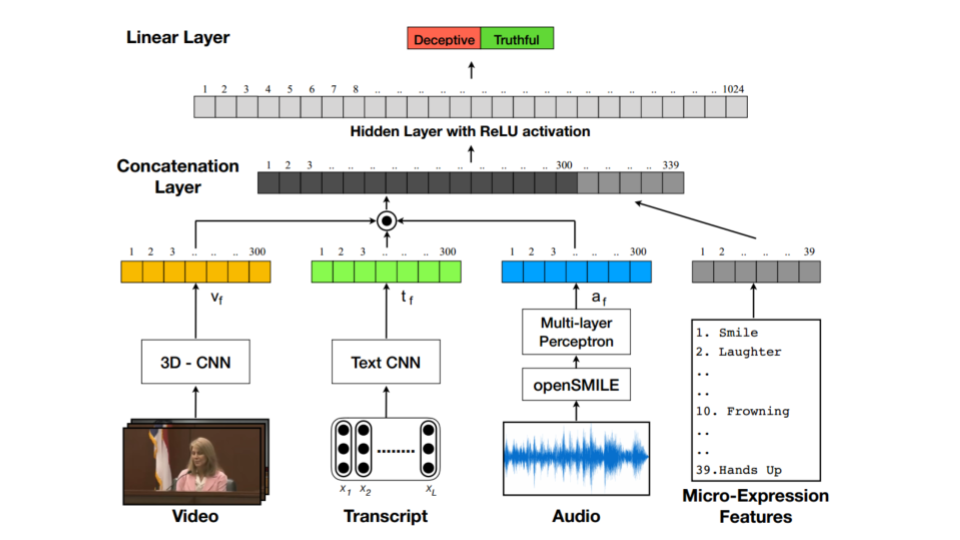
\includegraphics[width=13cm,keepaspectratio]{XX_Figures/Figura_Navonil_Modelo.png}
	\caption{\footnotesize Modelo de red neuronal multimodal utilizado por Krishnamurthy \cite{KrishnamurthyADetection}.}
	\label{fig:Figura_Navonil_Modelo}
\end{figure}

\begin{table}[h!]
\centering
    \begin{tabular}{|c|c|c|c|}
        \hline 
        Features & M LPu & MLPc & MLPh+c\tabularnewline
        \hline 
        \hline 
        Random & 43.90\% & 45.32\% & 48.51\%\tabularnewline
        \hline 
        Audio & 52.38\% & - & -\tabularnewline
        \hline 
        Visual & 93.08\% & - & -\tabularnewline
        \hline 
        Textutal (Static) & 80.16\% & - & -\tabularnewline
        \hline 
        Textual (Non-static) & 90.24\% & - & -\tabularnewline
        \hline 
        Micro-expressions & 76.16\% & - & -\tabularnewline
        \hline 
        All features (Static) & - & 90.49\% & 90.99\%\tabularnewline
        \hline 
        All features (Non\_static) & - & 95.24\% & 96.14\%\tabularnewline
        \hline 
    \end{tabular}
	\caption{\footnotesize Accuracy obtenido por Krishnamurthy con diferentes propuestas de modelos}
	\label{tab:Figura_Navonil_accuracy}
\end{table}

En este capítulo se presentaron varios estudios con diferentes propuestas no invasivas para detectar si una persona miente o no; estas propuestas obtienen mejores resultados para clasificar verdades y mentiras que el humano y algunos obtienen resultados similares al polígrafo. Vrij \cite{Vrij2000DetectingBehavior} a través de dos personas que extrajeron características manualmente en videos de personas mintiendo y diciendo verdades, anotando cuántas veces se desviaba la mirada, las veces que sonreía, movimientos de lo brazos y pies, etc, notaron que había diferencias en estas características entre las personas que decían mentiras y verdades, obteniendo una exactitud del 78\% para clasificar mentirosos y verdaderos. Verónica Pérez, una científica que ha trabajado en varios artículos que involucran la detección de mentiras junto con otros equipos, ha mostrado diferentes metodologías para clasificar verdades y mentiras de manera no invasiva. Además crearon un conjunto de datos que contienen personas mintiendo y diciendo verdades en juicios de Estados Unidos, el cual ha sido ocupado por algunos otros trabajos para detectar mentiras utilizando diferentes metodologías \cite{Perez-Rosas2015VerbalDetection,Abouelenien2016AnalyzingApproach}. Este conjunto de datos contiene a múltiples personas diciendo verdades y mentiras en la vida real, también se anotaron manualmente los gestos del rostro observados en los videos. A través de sistemas multimodales, combinando modalidades verbales y no verbales, Verónica y su equipo obtuvieron un 75\% de exactitud para clasificar verdades y mentiras en videos utilizando árboles de decisión. Después, con el uso de máquinas de soporte vectorial volvieron a probar un modelo multimodal pero utilizando dos conjuntos de datos, el que habían recopilado (`Trial') y uno nuevo que llamaron `Interview', ya que eran entrevistas hechas a diferentes personas en diferentes lugares. Ella y su equipo se dieron cuenta que cuando entrenaban su modelo con el conjunto de datos `Trial' y hacían las pruebas con el conjunto de datos `Interview' obtenían una exactitud del 58\% para clasificar los videos como verdad o mentira. A esta metodología de prueba se le llama Leave-one-person-out, la cuál esta basada en la validación cruzada leave-one-out con la diferencia que en lugar de dejar un conjunto de datos de prueba diferente al entrenamiento, se tienen personas diferentes en el conjunto de pruebas que en conjunto de entrenamiento. Utilizando la metodología Within-individual la cual se refiere a que en conjunto de pruebas y en el de entrenamiento se pueden encontrar las mismas personas, obtuvieron un 82\% para clasificar los datos del conjunto `Trial' y 79\% para el conjunto `Interview'. Krishnamurthy \cite{KrishnamurthyADetection} creando un sistema multimodal combinando información textual, visual, audio, microexpresiones manualmente anotadas y utilizando redes neuronales, fue capaz de clasificar videos como verdad o mentira con una exactitud del 96\% con la metodología de pruebas Leave-one-person-out en la que mencionan que las características que ayudaban a dar mejores resultados en el modelo multimodal eran las visuales las cuales fueron extraídas por una red convolucional 3D.
Otros trabajos se enfocaron en el uso de cámaras térmicas, tal es el caso de Abouelenien junto con Verónica \cite{Abouelenien2016AnalyzingApproach} en el cual crearon un sistema multimodal combinando el lenguaje no verbal, verbal y características térmicas convertidas a escala de grises y a HSV, obteniendo un 62\% de exactitud para clasificar verdades y mentiras. También Bashar \cite{Rajoub2014ThermalDetection} con el uso de cámaras térmicas y clasificación supervisada, logró clasificar verdades y mentiras con una exactitud del 58\% con la metodología Leave-one-person-out y 86\% con Within-individual utilizando árboles de decisión. Warmelink \cite{Warmelink2011ThermalAirports} construyó una herramienta computacional basada en la hipótesis en la que a través de imágenes térmicas, los mentirosos tienen una temperatura más alta que los verdaderos, obteniendo un 66\% para clasificar verdades y mentiras a través de respuestas fisiológicas medidas por cámaras térmicas.
En general se observa que diferentes trabajos han intentado solucionar el problema de detectar mentiras con métodos no invasivos y que deben existir características visuales que permiten a la computadora a través de diferentes extractores, instrumentos especiales, metodologías que involucran el movimiento del rostro, entre otros, obtener características importantes que permiten clasificar si una persona es deshonesto o es honesto en sus declaraciones. Esto motivó a que el presente trabajo se enfoque en el uso del lenguaje no verbal proporcionado por los fotogramas de un video y a utilizar aprendizaje profundo, ya que Krishnamurthy menciona tener mejores resultados para clasificar verdades y mentiras que las demás metodologías en el estado del arte utilizando aprendizaje profundo.

\begin{comment}
\ref{tab:ProblematicasPiloto}, se muestra una tabla de los diferentes métodos para detectar mentiras, la exactitud(accuracy) que tienen y las desventajas.

\begin{table}[h!]
\centering
    \begin{tabular}{|p{5cm}|p{2cm}|p{8cm}|}
        \hline 
        Método para detectar mentiras  & Accuracy  & Desventajas \tabularnewline
        \hline 
        \hline 
        Humanos no expertos & 54\%  & No conocen las pistas que delatan una mentira \tabularnewline
        \hline 
        Humanos expertos (Jueces, psicólogos, policias)  & 55\%  & Escenario interrogatorio, ver declaraciones varias veces, cada experto
        cree en diferentes pistas que delatan mentira, requieren de experiencia,
        high stake. \tabularnewline
        \hline 
        Polígrafo  & 70-95\%  & Ambiente controlado, calibración, horas para descifrar minutos, sistema
        invasivo, requiere de expertos, high stake. \tabularnewline
        \hline 
        Cámaras térmicas  & 64\%-87\%  & Ambiente controlado, calibración, costo elevado de material, high
        stake. \tabularnewline
        \hline 
        Lenguaje no verbal  & 60\%-96\%  & multimodales, algunos requieren de procesos manuales y requieren software
        especial. \tabularnewline
        \hline 
    \end{tabular}
    \caption{\footnotesize  Métodos para detectar mentiras.}.
    \label{tab:ProblematicasPiloto}
\end{table}
\end{comment}

\end{onehalfspacing}

    	%INCLUIR EL CAPÍTULO 4
		% Chapter 4
%----------------------------------------------------------------------------------------
\chapter{Propuesta de solución} % Main chapter title
\label{Chapter4} % For referencing the chapter elsewhere, use \ref{Chapter4} 
\begin{onehalfspacing}

\section{Metodología}
\label{sec:Metodologia}

La metodología que se presenta se basa en la hipótesis propuesta y en la Figura \ref{fig:Fig_Metodologia}, se muestra un esquema de la metodología que se utilizará para probar la hipótesis y a continuación una sección explicando cada uno de los pasos.

\begin{figure}[h!]
	\centering
	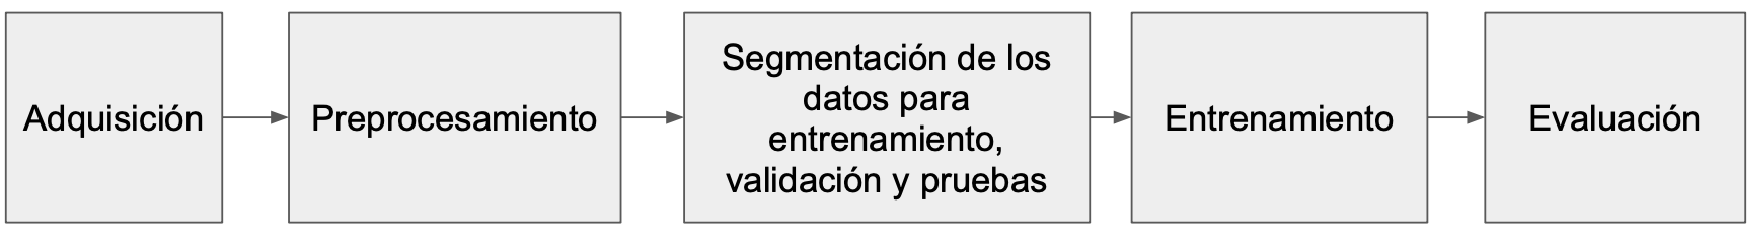
\includegraphics[width=18cm,keepaspectratio]{XX_Figures/Fig_Metodologia.pdf}
	\caption{\footnotesize Metodología propuesta para detectar mentiras en videos.}
	\label{fig:Fig_Metodologia}
\end{figure}

\subsection{Adquisición}
\label{sec:Adquisicion}
Al inicio se debe descargar o crear un conjunto de datos en la cuál se podrán hacer las pruebas de las hipótesis propuesta; este conjunto de datos debe contener videos con resoluciones medias tales cómo 480p o 720p(HD). Los formatos de los videos en WMV, MP4, MOV, AVI o FLV, con los 3 planos RGB. En los videos deben aparecer personas con declaraciones falsas y verdaderas. Estas personas también deben aparecer en todos los fragmentos del video para evitar el análisis de otros factores que no tengan que ver con el movimiento y la silueta del individuo. Nos podemos referir como \textit{frames} a los fotogramas que tiene un video ya que en varios trabajos en inglés y español es utilizado.\\

\subsection{Preprocesamiento}
\label{sec:Preprocesamiento}
Para el preprocesamiento de los videos se ocuparán librerías de OpenCV en python las cuáles han sido ocupadas para diferentes tareas que requieren de visión artificial, tales como reconocimiento de objetos, detección de movimientos, obtención de filtros espaciales, redimensionamiento, agudización de los frames, entre otros. A continuación se listan los pasos a seguir en el preprocesamiento:


\begin{enumerate}
    \item Obtener la separación de cada uno de los canales R,G,B Y la escala de grises promediada de cada uno de los fotogramas en los videos. La Figura \ref{fig:Fig_Dataset1_RGB_GS} muestra este procedimiento y la explicación de los canales RGB se encuentran la sección del Marco Teórico \ref{RGB} y para la obtención de la escala de grises en la sección del Marco Teórico \ref{GS}.
    \begin{figure}[h!]
    	\centering
    	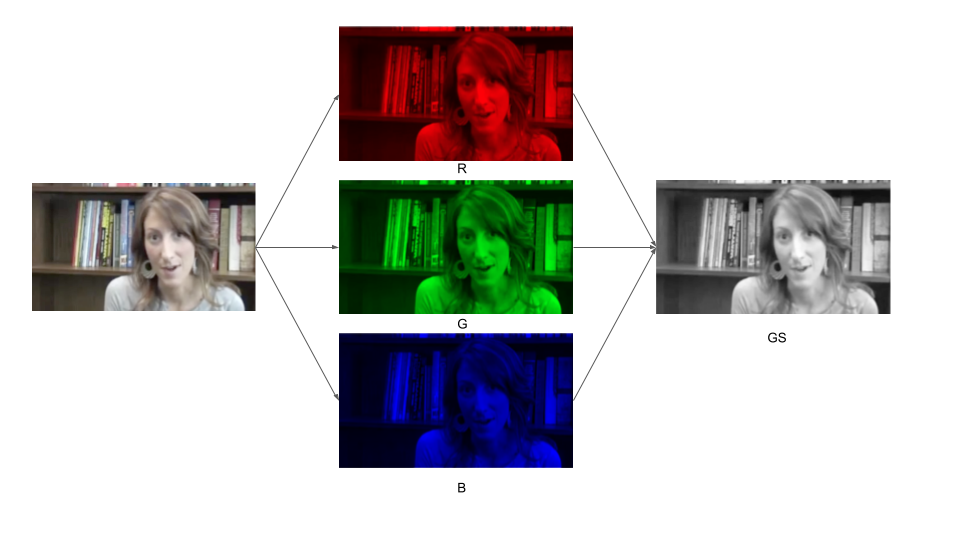
\includegraphics[width=10cm,keepaspectratio]{XX_Figures/Fig_Dataset1_RGB_GS.png}
    	\caption{\footnotesize Separación RGB y escala de grises.}
    	\label{fig:Fig_Dataset1_RGB_GS}
    \end{figure}
    
    \item Recortar los canales RGB de cada fotograma de los videos y la escala de grises (GS) obtenida para evitar tener información que no esté relacionada con el individuo a prueba. La primera propuesta de este recorte es quitando 60 píxeles en la parte superior, 70 en la parte inferior, 70 por la izquierda y 50 por la derecha. Al hacer este procedimiento se obtiene un fotograma como se muestra en la Figura \ref{fig:Fig_Dataset1_Recorte}. La segunda propuesta es recortar la imagen para obtener solamente el rostro del individuo; para lograr esto se utilizaron clasificadores en cascada basados en funciones de Haar, el cuál a través de aprendizaje profundo, la función de cascada se entrena a través de gran cantidad de imágenes positivas (imágenes con caras) y negativas (imágenes sin caras) para luego ser utilizada en detección de rostros en otras imágenes.  
    \begin{figure}[h!]
    	\centering
    	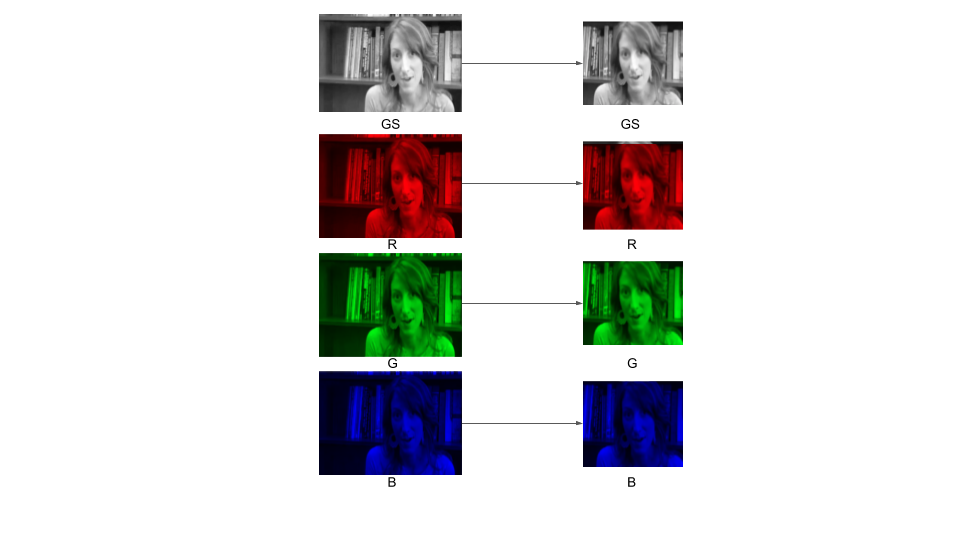
\includegraphics[width=12cm,keepaspectratio]{XX_Figures/Fig_Dataset1_Recorte.png}
    	\caption{\footnotesize Recorte de los fotogramas.}
    	\label{fig:Fig_Dataset1_Recorte}
    \end{figure}

    \item Aplicar redimensión a R,G,B y GS para reducir el tamaño de los datos con el costo de perder calidad de información pero reduciendo el costo computacional de las operaciones que se realizarán a cada uno de los fotogramas. Para el redimensionamiento se ocupará la función \textit{resize} de la librería de OpenCV, con interpolación \textit{InterArea} la cuál obtiene el promedio de gran cantidad de píxeles. Esta interpolación es muy útil para achicar una imagen pero mala para agrandarla. Al final de este procedimiento se obtiene una imagen de (y,x) píxeles. En la Figura \ref{fig:Fig_Dataset1_Redimensionar} se muestra un ejemplo de un fotograma extraído de un video en HD para obtener un fotograma con tamaño 100 x 100.
    \begin{figure}[h!]
    	\centering
    	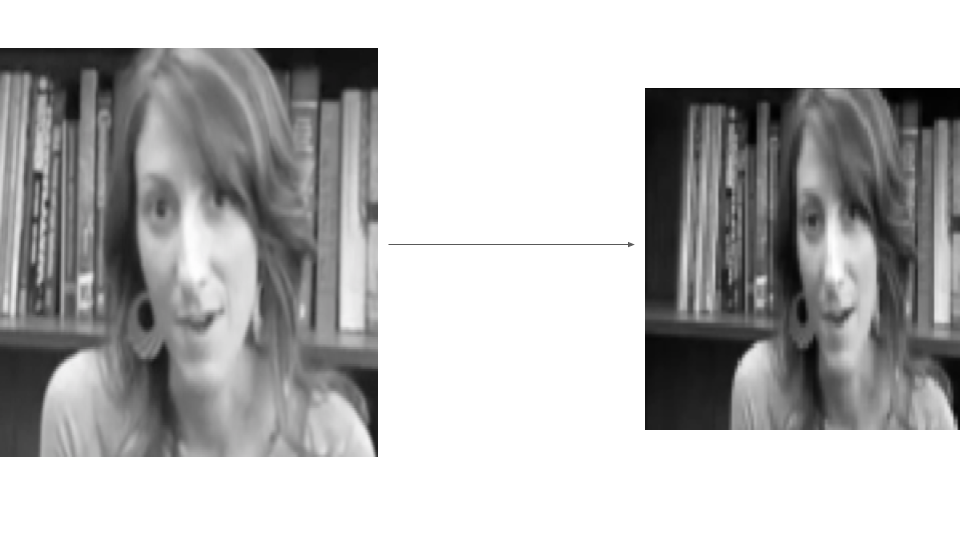
\includegraphics[width=12cm,keepaspectratio]{XX_Figures/Fig_Dataset1_Redimensionar.png}
    	\caption{\footnotesize Redimensionamiento de los fotogramas de un video HD (1280x720) a 100x100 pixeles.}
    	\label{fig:Fig_Dataset1_Redimensionar}
    \end{figure}

    \item Aplicar los filtros SobelX (SX), SobelY(SY) y Kirsh (K) para obtener las siluetas y bordes de los objetos, OpticalFlowX(OX) y OpticalFlowY(OY) para obtener el movimiento de un fotograma con respecto a otro consecutivo y Laplaciano (L) para agudizar los fotogramas. Cada uno de estos filtros son explicados en la sección \ref{Filtros_espaciales} del Marco Teórico. En la Figura \ref{fig:Fig_Dataset1_Filtros} se muestra un ejemplo de la obtención de estos filtros con el filtro escala de grises (GS).
    \begin{figure}[h!]
    	\centering
    	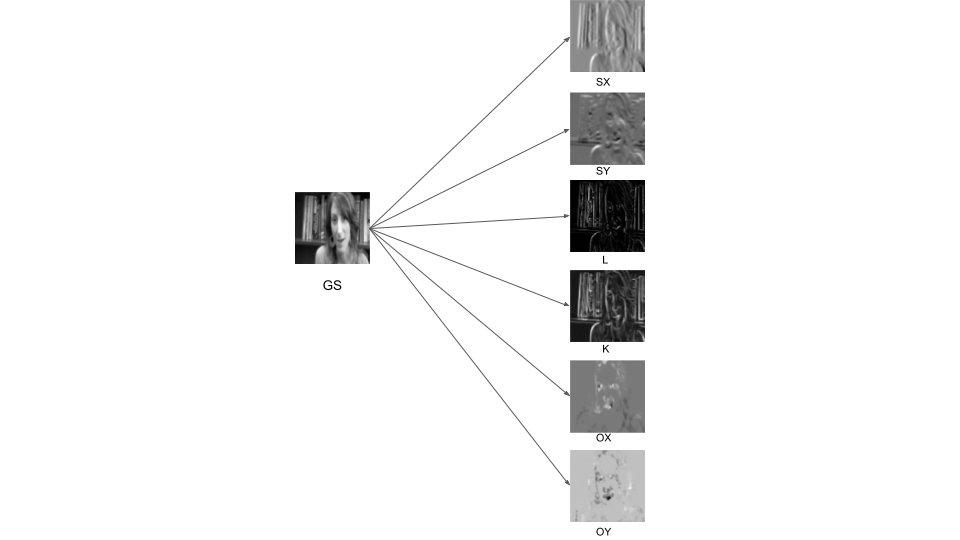
\includegraphics[width=18cm,keepaspectratio]{XX_Figures/Fig_Dataset1_Filtros.png}
    	\caption{\footnotesize Obtención de los canales SX,SY,OX,OY,L y K.}
    	\label{fig:Fig_Dataset1_Filtros}
    \end{figure}
    
    \item División de los videos en fragmentos: Cada uno de los videos se fragmentará en n número de fotogramas, ya que se desea probar si con pequeños fragmentos de videos con n número de fotogramas es suficiente para reconocer mentira o verdad en una persona. Los formatos y la cantidad de fotogramas por segundo que tiene un video pueden cambiar, por ejemplo si se tiene un video a 30 FPS (60 Hz), se puede convertir a 15 FPS si se toman la mitad de los fotogramas del video a 30 FPS pero con la misma cantidad de tiempo; esto se puede lograr tomando como separación un fotograma entre cada fotograma que se ocupe. A este procedimiento lo llamaremos \textbf{FrameSpace} y se refiere a la cantidad de espacios (fotogramas) que hay entre los fotogramas seleccionados, este procedimiento se puede apreciar en la Figura \ref{fig:Fig_FrameSpace} y se utilizará para saber a que velocidad de fotogramas se pueden detectar mentiras y verdades. Al final de este proceso se obtendrá lo que llamaremos un \textbf{dato}, el cual consiste en n cantidad de fotogramas, con c cantidad de canales y dimensión espacial (y,x). En la Figura \ref{fig:Fig_Dato7Frames}, se observa un ejemplo de un dato x que contiene n = 7 fotogramas, c = 3 canales (RGB), (y,x) = 100x100 píxeles. Schindler \cite{SchindlerVanRequire} menciona que de 1 a 7 fotogramas a 25 Hz (25 Hz $\simeq$ 13 FPS) es suficiente para reconocer acciones humanas y en \cite{Ji20133DRecognition} solamente necesitaron de 7 fotogramas para detectar acciones humanas con una mayor precisión que tomando todo los fotogramas de un video, esto motivó a que el modelo piloto tuviera como entrada datos de 7 fotogramas y los canales RGB.
    
    \begin{figure}[h!]
    	\centering
    	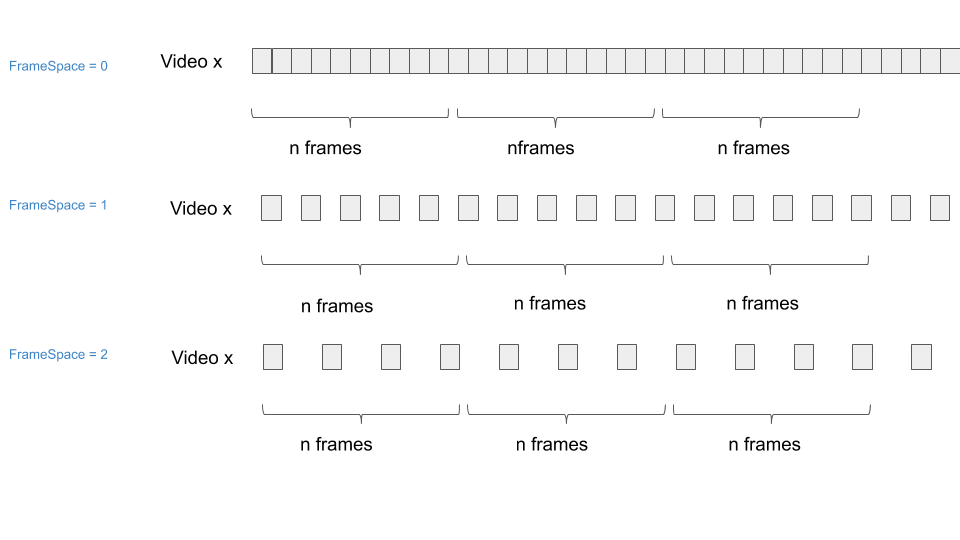
\includegraphics[width=14cm,keepaspectratio]{XX_Figures/Fig_FrameSpace.png}
    	\caption{\footnotesize Funcionamiento de FrameSpace.}
    	\label{fig:Fig_FrameSpace}
    \end{figure}
    
    \begin{figure}[h!]
    	\centering
    	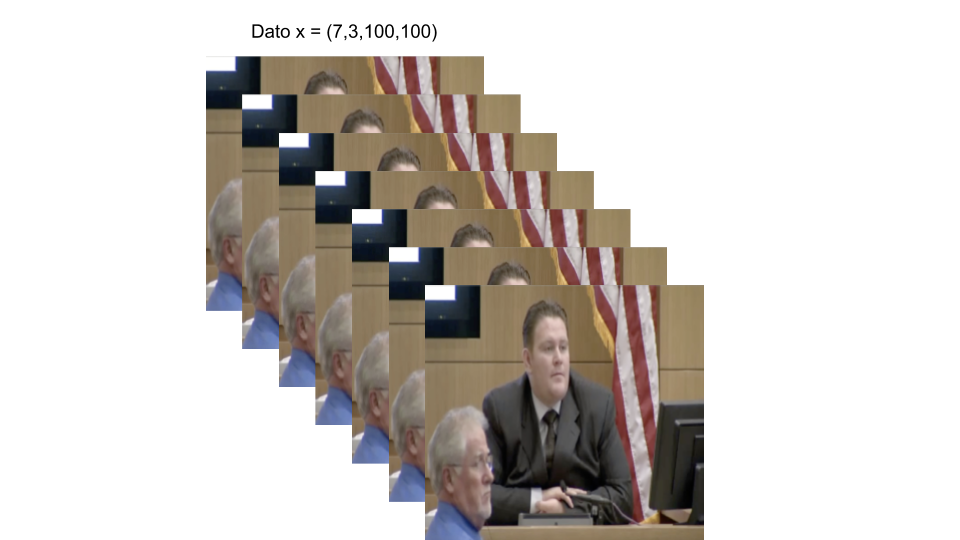
\includegraphics[width=12cm,keepaspectratio]{XX_Figures/Fig_Dato7Frames.png}
    	\caption{\footnotesize Ejemplo de un dato.}
    	\label{fig:Fig_Dato7Frames}
    \end{figure}
    
    \item Cada uno de los datos se etiquetan con [1,0] en el caso de pertenecer a un video de mentira o [0,1] en el caso de pertenecer a un video de verdad. En la Figura \ref{fig:Fig_Etiqueta_datos} se muestra un ejemplo en la que \textit{m} datos pertenecientes a un video de mentira son etiquetados con [1,0] indicando que son datos de mentira y \textit{v} datos pertenecientes a un video de verdad son etiquetados con [0,1] indicando que son datos de verdad.
\end{enumerate}

\begin{figure}[h!]
    	\centering
    	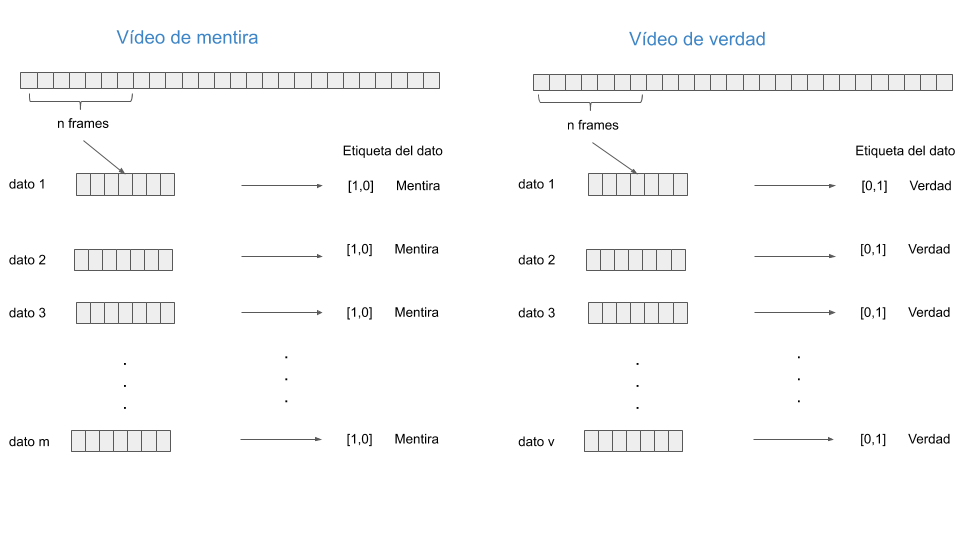
\includegraphics[width=17cm,keepaspectratio]{XX_Figures/Fig_Etiqueta_datos.png}
    	\caption{\footnotesize Etiquetado de los datos.}
    	\label{fig:Fig_Etiqueta_datos}
\end{figure}

%---------------------------------------------
\subsection{Segmentación de los datos}
\label{sec:Segmentacion datos}
Los datos se segmentarán de la siguiente manera: 
\begin{itemize}
    \item  El primero conjunto de datos es el Train en el cuál están la mayoría de los datos; esto es para que se la red tenga suficientes datos que le permitan generalizar o al menos conocer las suficientes situaciones en las que necesite clasificar nuestro problema. Estos datos de entrenamiento contienen \textit{D} datos etiquetados como mentira y \textit{T} datos etiquetados como verdad los cuales serán barajeados (shuffle) aleatoriamente. Una vez combinados los \textit{n} datos de entrenamiento, se dividirán en lotes (batches) con \textit{m} cantidad de datos. Cada uno de los batches pasarán por las etapas de entrenamiento explicadas posteriormente en la subsección \ref{sec:Entrenamiento} y al terminar de pasar todos los batches, habrá terminado la primera época de entrenamiento. Este procedimiento se repite \textit{e} cantidad de veces, dependiendo del número de épocas. Entre más grande sea el tamaño del batch, más capacidad computacional será necesaria para entrenar los datos.
    \item El segundo conjunto es el Validation en la cuál se extrae un pequeño conjunto de datos del Train para notar como se comporta la red con datos muy parecidos pero nunca antes vistos. Este conjunto se evalúa al terminar una época de entrenamiento.
    \item El último conjunto es el Test en la cuál se harán las pruebas para conocer la robustez y la confiabilidad del sistema; aquí por lo general los datos son diferentes que el conjunto de Train y Validation. Este conjunto se evalúa después de e épocas propuestas.
\end{itemize}

\subsection{Entrenamiento}
\label{sec:Entrenamiento}

\subsubsection{Entradas y salidas}
\label{sec:Entrada}

Para la entrada al modelo los datos consistirán en \textit{d = (f,c,y,x)} en dónde \textit{f = número de fotogramas}, \textit{c = número de canales}, y \textit{(y,x)= (altura,ancho)} del fotograma.\\
Debido a que se tiene una codificación \textit{One Hot} en las etiquetas de cada dato como se muestra en la Figura \ref{fig:Fig_Etiqueta_datos}, al final el modelo dará como salida un vector con dos valores, en la cuál el valor más grande representará cómo fue clasificado el dato.

\subsubsection{Arquitectura}
\label{sec:Arquitectura}

Al inicio de la arquitectura, los datos \textit{d = (f,c,y,x)} pasarán por una red convolucional 3D que será la encargada de la extracción de características. Se desea tener un vector \textit{v} a la salida de la red convolucional 3D, por lo tanto dependiendo de dimensiones espaciales en los fotograma \textit{(y,x)}, combinaciones de canales \textit{c} y cantidad de fotogramas \textit{f}, pueden variar la cantidad de capas convolucionales y maxpooling, dando como resultado diferentes arquitecturas. el vector de características \textit{v} se convertirá en la entrada de las capas completamente conectadas en cuál tendrá $C_{mlp}$ capas con diferentes números de neuronas y diferentes funciones de activación. Al final se tendrá una capa de salida con dos neuronas. Con fines visuales, para la arquitectura mostrada a continuación se ocupó como entrada datos de 7 fotogramas con 3 canales (R,G,B) y con dimensiones espaciales de 100x100 píxeles, con el fin de explicar el funcionamiento de la red 3DCNN. Por lo tanto los datos tienen los siguientes valores $${d = (7,3,100,100)}$$ Los pasos se describen a continuación:\\

\begin{enumerate}
    \item Cada uno de los canales se agrupa por separado con sus 7 fotogramas correspondientes, para posteriormente aplicar los filtros convolucionales 3D a cada canal por separado (Figura \ref{fig:Fig_Piloto_p1}).
    
    \begin{figure}[h!]
	\centering
	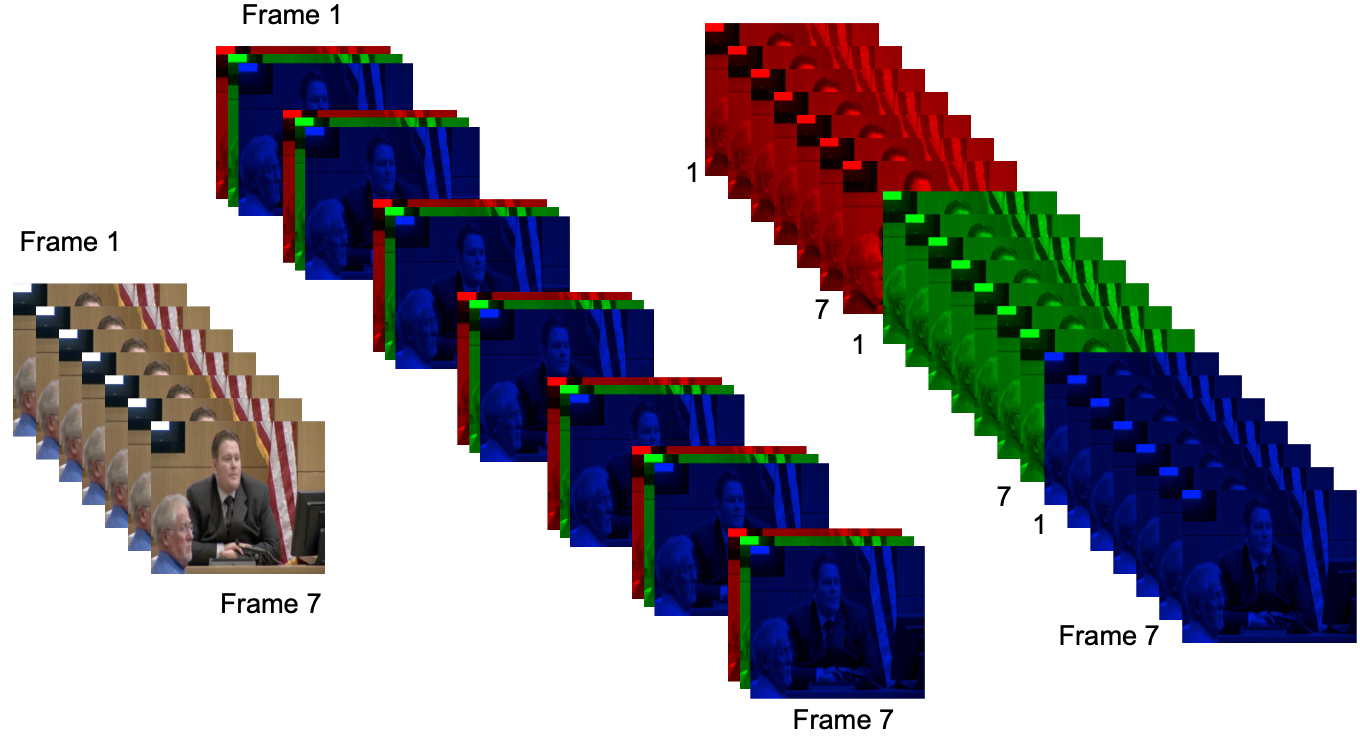
\includegraphics[width=9cm,keepaspectratio]{XX_Figures/Fig_Piloto_p1.png}
	\caption{\footnotesize Separación y agrupación de los canales R,G,B para el modelo piloto.}
	\label{fig:Fig_Piloto_p1}
    \end{figure}
    
    \item Se toma uno de los canales \textit{c} y se le aplicarán \textit {k} kernels convolucionales con dimensión $C = (t_{c},c_{c},x_{c},y_{c})$. Para este ejemplo \textit{k = 4} y cada kernel en esta primera capa convolucional $C1(t,c,y,x) = C1(3,1,3,3)$, tienen un tamaño de $3x3$ en altura y anchura, con una profundidad de canal $c_{c} = 1$(que indica que se aplica la 3DCNN por separado a cada canal) y con dimensión $t_{c}=3$ que indica que se tomarán 3 fotogramas para realizar el paso convolucional. Al aplicar el filtro convolucional 3D con \textit{TemporalStride = 1 y Padding = Same} (sin relleno) se obtienen 4 conjuntos mapas de características, cada uno con 5 matrices y con una anchura y altura de 98x98 respectivamente como se muestra en la Figura \ref{fig:Fig_Piloto_p2}. 
    \begin{figure}[h!]
	\centering
	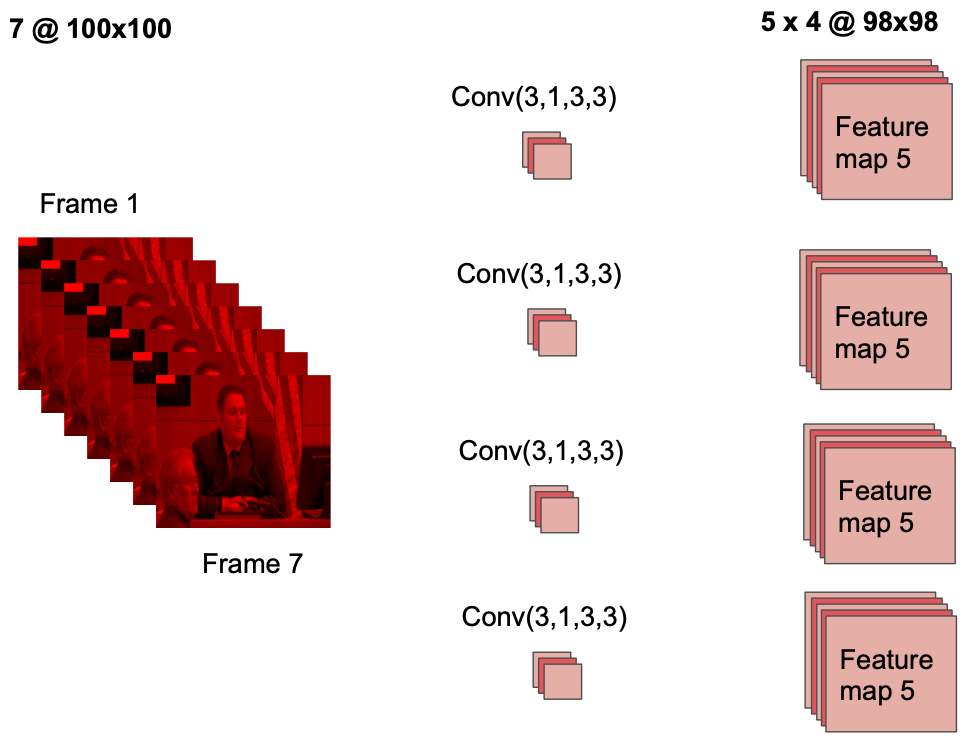
\includegraphics[width=7cm,keepaspectratio]{XX_Figures/Fig_Piloto_p2.png}
	\caption{\footnotesize Aplicación de C1.}
	\label{fig:Fig_Piloto_p2}
    \end{figure}
    
    \item Se aplica un Maxpooling M1 de tamaño \textit{M1(t,y,x) = M1(1,2,2)}, el cual da como resultado los mismos conjuntos de mapas de características pero con una anchura y altura de 49x49 como se muestra en la Figura \ref{fig:Fig_Piloto_M1}.\\
    \begin{figure}[h!]
	\centering
	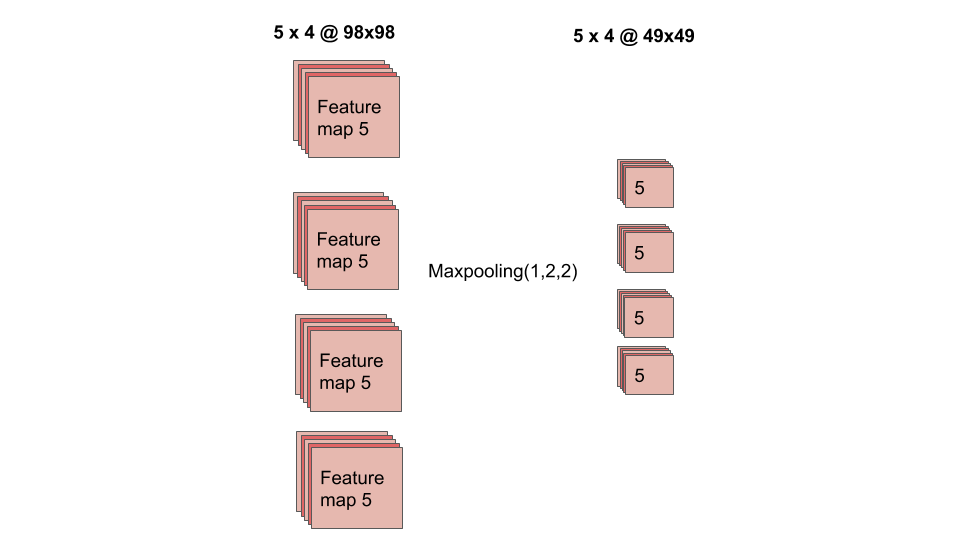
\includegraphics[width=12cm,keepaspectratio]{XX_Figures/Fig_Piloto_M1.png}
	\caption{Aplicación de M1.}
	\label{fig:Fig_Piloto_M1}
    \end{figure}
    
    \item Después se volvieron a aplicar 4 kernels convolucionales 3D pero con valores \textit{C2(3,1,5,5)}, y las mismas características de TemporalStride y Padding. Esto da como resultado 16 conjuntos de mapas de características con 3 matrices cada uno y un tamaño de 45x45 como se muestra en la Figura \ref{fig:Fig_Piloto_C2}.
    \begin{figure}[h!]
	\centering
	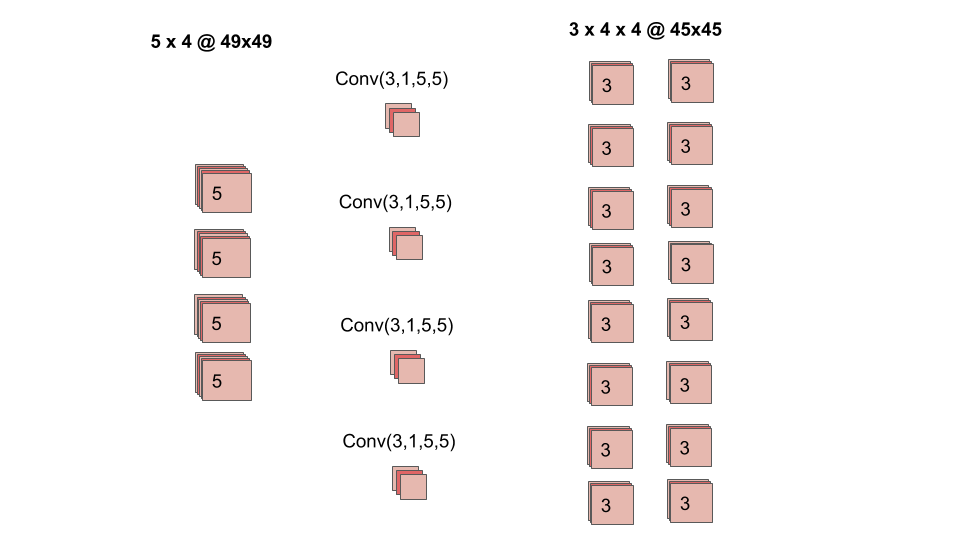
\includegraphics[width=12cm,keepaspectratio]{XX_Figures/Fig_Piloto_C2.png}
	\caption{\footnotesize Aplicación de C2.}
	\label{fig:Fig_Piloto_C2}
    \end{figure}
    
    \item Se aplica un Maxpooling M2 de tamaño \textit{M2(1,5,5)}, el cual da como resultado los mismos conjuntos de mapas de características pero con una anchura y altura de 9x9 respectivamente como se muestra en la Figura \ref{fig:Fig_Piloto_M2}. 
    \begin{figure}[h!]
	\centering
	\includegraphics[width=14cm,keepaspectratio]{XX_Figures/Fig_Piloto_M2.png}
	\caption{\footnotesize Aplicación de M2.}
	\label{fig:Fig_Piloto_M2}
    \end{figure}
    
    \item Luego se aplican 2 kernels convolucionales 3D \textit{C3(3,1,5,5)} para obtener 32 conjuntos de mapas de características con 1 matriz por cada conjunto y una dimensión espacial de 5x5 como se muestra en la Figura \ref{fig:Fig_Piloto_C3}.
    \begin{figure}[h!]
	\centering
	\includegraphics[width=15cm,keepaspectratio]{XX_Figures/Fig_Piloto_C3.png}
	\caption{\footnotesize Aplicación de C3.}
	\label{fig:Fig_Piloto_C3}
    \end{figure}
    
    \item Se aplica un Maxpooling M2 de tamaño \textit{M2(1,5,5)} para obtener un vector con 32 características, las cuales fueron extraídas de un canal con 7 fotogramas (Figura \ref{fig:Fig_Piloto_p5}).
    \begin{figure}[h!]
	\centering
	\includegraphics[width=13cm,keepaspectratio]{XX_Figures/Fig_Piloto_p5.png}
	\caption{\footnotesize Aplicación de C5 para obtener vector de características de 32 valores.}
	\label{fig:Fig_Piloto_p5}
    \end{figure}
    
    \item Este mismo procedimiento es aplicado para cada uno de los tres canales y se obtiene un resultado similar como se puede apreciar en la Figura \ref{fig:FIG_3DCNN_DATASET1}, en la cual se muestra al final del proceso los 3 vectores de características obtenidos por los 3 filtros concatenados. Este procedimiento puede ser aplicado para n canales.
    \begin{figure}[h!]
	\centering
	\includegraphics[width=16cm,keepaspectratio]{XX_Figures/FIG_3DCNN_DATASET1.png}
	\caption{\footnotesize Red convolucional 3D.}
	\label{fig:FIG_3DCNN_DATASET1}
    \end{figure}
    
    \item El vector de características concatenado se vuelve la entrada a una MLP profunda con 2 capas ocultas con 96 y 128 neuronas respectivamente y una capa de salida con dos neuronas. Al final se tendrá una clasificación, la cuál será comparada con la etiqueta real. Reduciendo el error obtenido hasta que nuestra condición de paro suceda (Figura \ref{fig:Fig_3DDNN_Piloto}).
    \begin{figure}[h!]
	\centering
	\includegraphics[width=18cm,keepaspectratio]{XX_Figures/Fig_3DDNN_Piloto.png}
	\caption{\footnotesize Arquitectura completa DNN propuesta.}
	\label{fig:Fig_3DDNN_Piloto}
\end{figure}
    
\end{enumerate}


Con este ejemplo se observa que dependiendo de los datos, se pueden construir diferentes modelos con diferentes variedades de filtros convolucionales, capas convolucionales, TemporalStrides, ConvStrides, MaxPoolStrides, etc. De igual forma se pueden construir MLPs con diferentes funciones de transferencia, números de neuronas y de capas ocultas, etc.

\subsubsection{Ajuste de hiperparámetros de entrenamiento}
\label{sec:ajustehiperparametros}
Para calcular el error de salida obtenido por el modelo, se ocupa la función de entropía cruzada (Cross-Entropy). Esta función mide el rendimiento del modelo de clasificación cuyo resultado es un valor de probabilidad entre 0 y 1. La pérdida de entropía cruzada (cross-entropy loss) aumenta a medida que la probabilidad predicha diverge de la etiqueta real y esta es calculada con la ecuación \ref{equ:crossentropy}, donde $p(x)$ es la probabilidad deseada y $q(x)$ es la probabilidad actual. Para disminuir el error obtenido se utilizará el optimizador Adam con valores de Learning rate iniciales entre 0.01 y 0.0001.

\begin{equation}
\label{equ:crossentropy}
    H(p,q) = -\sum_{x}p(x)\log q(x)
\end{equation}



\subsection{Evaluación}
\label{sec:Evaluacion}

Al final de el modelo se debe de evaluar que tan acertado es para detectar mentiras y verdades. La métrica comúnmente utilizada por el estado del arte es la exactitud (accuracy) la cuál es el promedio de los datos clasificados correctamente \cite{Bond2006AccuracyJudgments,Vrij2000DetectingBehavior,Perez-Rosas2015VerbalDetection,KrishnamurthyADetection}. Por ejemplo imaginemos que tenemos 10 datos, 5 son datos con la etiqueta de mentira y 5 con la etiqueta de verdad; El sistema nos arroja que logró clasificar 4 mentiras y 3 verdades correctamente, entonces la exactitud del modelo es de 0.70, convertido a porcentaje es 70\%. Esta exactitud por dato se calcula con la Ecuación \ref{equ:Accuracy}. Se puede referir como \textit{accuracy} a la exactitud.\\

\begin{equation}
\label{equ:Accuracy}
    AccuracyData = \frac{TP+TN}{TP+TN+FP+FN} = \frac{DatosClasificadosCorrectamente}{DatosTotales}
\end{equation}\\


Una propuesta para evaluar el desempeño de los modelos es utilizando una nueva métrica la cuál no evalúa los datos clasificados correctamente, si no que considera los videos que fueron clasificados correctamente. Esta métrica se propuso ya que decidir si una persona mintió o dijo la verdad en todos los fragmentos en los que se segmentó el video podría convertirse en una tarea difícil de clasificar para el modelo.- Para decidir si un video compuesto de n datos es clasificado correctamente se propone que si un video tiene (n/2 + 1) datos clasificados como mentira, entonces hay más probabilidad de que el video pertenezca a esa clase y viceversa.
Al final se obtendrá un accuracy por videos, mostrados por la Ecuación \ref{equ:AccPerVideo}.\\

\begin{equation}
\label{equ:AccPerVideo}
    AccuracyPerVideo = \frac{AccVideo_{0} + AccVideo_{1} + ... + AccVideo_{m}}{m}
\end{equation}\\

donde m es el total de los videos y AccVideo puede tomar 1 si fue clasificado como correcto o como incorrecto.


\section{Datasets}
\label{sec:Datasets}

\subsection{Dataset `Trial'}
\label{sec:Dataset-Trial}

\begin{figure}[th]
	\centering
	\includegraphics[width=17cm,keepaspectratio]{XX_Figures/Fig_Dataset1.png}
	\caption{\footnotesize Algunos fotogramas de los videos del dataset utilizado en el modelo piloto.}
	\label{fig:Fig_Dataset1}
\end{figure}

El dataset que se propone utilizar ha sido utilizado anteriormente por algunos artículos enfocados a detectar mentiras a través de video \cite{Perez-Rosas2015VerbalDetection,Wu2018DeceptionVideos,KrishnamurthyADetection}. En la Figura \ref{fig:Fig_Dataset1} se observan algunos fotogramas extraídos de 8 videos distintos del dataset `Trial' con diferentes personas, diferentes enfoques y diferentes escenarios. Este conjunto de datos contiene las siguientes características:\\

\begin{itemize}
    \item 121 videos de cortes de Estados Unidos con mentiras y verdades en la vida real.
    \item Los datos están en formato RGB, 30 Fotogramas por segundo (30 FPS), MP4 y 1280x720.
    \item Los videos tienen diferentes individuos (hombres y mujeres en su gran mayoría caucásicos).
    \item El dataset muestra a pocos individuos diciendo mentiras y verdades (6 individuos)
    \item Los videos no están equilibrados en tiempo.
\end{itemize}

\begin{figure}[th]
	\centering
	\includegraphics[width=9cm,keepaspectratio]{XX_Figures/Fig_Dataset1_Venn.png}
	\caption{\footnotesize Diagrama de Venn del dataset piloto.}
	\label{fig:Fig_Dataset1_Venn}
\end{figure}

Por la poca cantidad de videos se decidió que en el conjunto de Test hubiera personas distintas en lugar de declaraciones ya que a pesar de que varias personas aparecían en diferentes videos con diferentes declaraciones, éstas solo aparecían en una sola clase (verdad o mentira). Adicionalmente se obtuvieron más videos de los 121 videos que contenía el dataset "Trial" (Figura \ref{fig:Fig_Dataset1}), ya que algunos videos tenían lapsos de tiempo en la que el sujeto no aparecía en la escena y se dividió en un nuevo video por cada lapso nuevo en la que no aparecía el individuo; de esta manera se obtuvieron más videos y se eliminaron datos sin importancia.
En la Figura \ref{fig:Fig_Dataset1_Venn} se observa un diagrama de Venn de como están distribuidos los videos en el Dataset `Trial'. en verde se observa que se tienen 66 videos con 34 personas distintas etiquetadas como verdad, en rojo 67 videos con 19 individuos etiquetadas como mentira y en la intersección se encuentran 32 videos con 6 individuos que aparecen con la etiqueta de verdad y otros con la etiqueta de mentira.

Para el entrenamiento y pruebas de desempeño de la red, los datos se dividieron de la siguiente manera:

\begin{itemize}
    \item Train: 106 videos para los datos de entrenamiento.
    \item Validation: Este conjunto de datos se obtuvo extrayendo datos un 10 \% de los datos de Train por lo tanto contiene mismas personas que en el conjunto de Train.
    \item Test: 27 videos para los datos de prueba.  Este conjunto de datos contiene diferentes personas y declaraciones que en el conjunto de Train y Validation.
\end{itemize}

%---------------------
%---------------------
%---------------------


\subsection{Dataset `Interview'}
\label{sec:DatasetInterview}

Este nuevo conjunto de datos ha sido utilizado por su Lloyd \cite{Lloyd2019MiamiDatabase} para probar la hipótesis de que las personas tienden a juzgar de diferente manera a las razas para decidir si mienten o dicen la verdad; Las personas obtuvieron una exactitud de 54\% para detectar mentiras y verdades \cite{Lloyd2019MiamiDatabase}. La cantidad de videos que contiene es casi el triple que el anterior dataset ocupado y está más equilibrado en tiempo, videos y personas. A continuación se listan las características de este conjunto:\\


\begin{itemize}
    \item 320 videos de aproximadamente 30s de personas con declaraciones falsas y verdades. .
    \item Los datos están en formato RGB, 30 Fotogramas por segundo (30 FPS), MP4 y 1280x720.
    \item hay 80 individuos diferentes en donde 20 son hombres blancos, 20 hombres negros, 20 mujeres blancas y 20 mujeres negras. Cada individuo contiene 4 videos; 2 videos con distintas declaraciones de verdad y 2 videos con distintas declaraciones de mentira.
    \item En todos los video solo aparecen los mismos sujetos sin movimiento de la cámara.
\end{itemize}

En la Figura \ref{fig:Fig_Dataset2} se muestran 16 fotogramas extraídos de 16 videos distintos. Cada uno de los 4 fotogramas pertenecientes al mismo individuo pero a diferente video muestran el mismo fondo, la misma ropa y en general el mismo ambiente.

\begin{figure}[h!]
	\centering
	\includegraphics[width=6cm,keepaspectratio]{XX_Figures/Fig_Dataset2.png}
	\caption{\footnotesize Algunos fotogramas del Dataset `Interview'}
	\label{fig:Fig_Dataset2}
\end{figure}

En el Capítulo \ref{Chapter3} se menciona que Bashar A. Rajoub en Junio del 2014 \cite{Rajoub2014ThermalDetection}, obtuvo un pobre desempeño predictivo al segmentar los datos con la metodología \textit{leave-one-person-out} en la que los individuos de los datos de prueba eran distintos a los individuos de los datos de entrenamiento, pero obtuvo excelentes resultados con la metodología \textit{within-indidivual} en la que los individuos de los datos de entrenamiento también se encontraban en los datos de prueba pero con diferentes declaraciones.\\

Como este conjunto de datos es casi tres veces más grande que el dataset `Trial' y equilibrado en personalidades y duración, se decidió dividir los datos de prueba en TestWI y TestPO para probar si se obtenían resultados similares con las dos metodologías que Bashar A. Rajoub y otros artículos obtuvieron . Se segmentaron los datos de la siguiente manera (Figura \ref{fig:Fig_Dataset2_Segmentos}):

\begin{figure}[th]
	\centering
	\includegraphics[width=10cm,keepaspectratio]{XX_Figures/Fig_Dataset2_Segmentos.png}
	\caption{\footnotesize Segmentos propuestos del Dataset `Interview' para los modelos propuestos.}
	\label{fig:Fig_Dataset2_Segmentos}
\end{figure}

\begin{itemize}
    \item \textbf{Train}: 254 videos (79.3\%): En la ecuación \ref{equ:Train}, se observa cómo esta compuesto el conjunto de entrenamiento. Este conjunto de entrenamiento contiene un total de 70 personas diferentes, 57 con 4 videos diferentes (2 con declaraciones de verdad y 2 de mentira) y 13 personas con 2 videos diferentes (1 de verdad y 1 de mentira)
    \begin{equation}
    \label{equ:Train}
        Train = 57_{personas} * 4_{V,V,M,M} + 13_{personas} * 2_{V,M}
    \end{equation}
    
    \item \textbf{Test within-indidivual (TestWI)}: 26 videos (8\%): En la ecuación \ref{equ:TestWI}, se observa cómo esta compuesto el conjunto de pruebas TestWI. Este conjunto de pruebas contiene 13 personas distintas y son personas que también se encuentran en el conjunto de entrenamiento pero con diferentes videos y declaraciones.
    \begin{equation}
    \label{equ:TestWI}
        TestWI = 13_{personas} * 2_{V,M}
    \end{equation}
    
    \item \textbf{Test leave-one-person-out (TestPO)}: 40 videos (12.7\%): En la ecuación \ref{equ:TestPO}, se observa cómo esta compuesto el conjunto de pruebas TestPO. Este conjunto de pruebas contiene 20 personas y son personas distintas al conjunto de entrenamiento.
    \begin{equation}
    \label{equ:TestPO}
        TestPO = 20_{personas} * 4_{V,V,M,M}
    \end{equation}
    
\end{itemize}

%---------------------------------
%---------------------------------

\section{Nomenclatura}
\label{sec:Nomenclatura}

En esta sección se explicará la nomenclatura que se ocupa para los diferentes modelos utilizados en las siguientes secciones. Algunos de estos conceptos ya se encuentran explicados en el Capítulo \ref{Chapter2}. Al comienzo de cada modelo se tendrá 3D que indica que la arquitectura está basada en redes neuronales convolucionales 3D. lo primero en aplicarle a la entrada de todos los modelos será una capa convolucional, seguida por una capa maxpooling y en caso de tener varias capas convolucionales y varias capas maxpooling, seguiran teniendo la estructura (C1,M1,C2,M3,C3,...,Cn) o (C1,M1,C2,M3,C3,...,Mn), Cn representando la capa convolocional n y Mn la n capa maxpooling. Para todos los modelos se aplicaron los filtros convolucionales a los canales por separado, por lo tanto la profundidad de canales de los kernels en todos los modelos es de 1. También se utilizo el optimizador Adam y la función de perdida Cross Entropy.

\begin{itemize}
    \item  {[ID]\textbf{DS}}: Indica el dataset que se está ocupando en el modelo y el preprocesamiento personalizado que tuvo. Los valores de DS se encuentran en la tabla \ref{tab:DS}.
    \begin{itemize}
        \item Dataset: Dataset que se está ocupando.
        \item  FrameSize: Tamaño espacial de los fotogramas.
        \item ObjectFrame: objetos que se encuentran en la mayoría de los fotogramas al terminar el preprocesamiento.
    \end{itemize}
    
    \begin{table}[h!]
    \centering
    \begin{tabular}{|c|c|c|c|}
        \hline 
        ID\_DS & Dataset & FrameSize & ObjectFrame\tabularnewline
        \hline 
        \hline 
        {[}1{]} & Trial & 100x100 & Face,shoulders,arms\tabularnewline
        \hline 
        {[}2a{]} & Interview & 50x50 & Face,shoulders,arms\tabularnewline
        \hline 
        {[}2b{]} & Interview & 50x50 & Face\tabularnewline
        \hline 
        {[}2c{]} & Interview & 100x100 & Face,shoulders,arms\tabularnewline
        \hline 
    \end{tabular}
    \caption{\footnotesize IDs de \textbf{DS}.}.
    \label{tab:DS}
    \end{table} 
    
    %----------------------------------------------------------------------------
    \item {[ID]\textbf{CH}}: Combinación de canales ocupados por el modelo. Los valores de CH se encuentran en la tabla \ref{tab:CH}.
    \begin{table}[h!]
    \centering
    \begin{tabular}{|c|c|}
        \hline 
        [ID]CH & Channels\tabularnewline
        \hline 
        \hline 
        {[}0{]} & R,G,B\tabularnewline
        \hline 
        {[}1{]} & GS,KIR,LAP\tabularnewline
        \hline 
        {[}2{]} & GS,OX,OY\tabularnewline
        \hline 
        {[}3{]} & GS,SX,SY\tabularnewline
        \hline 
        {[}4{]} & GS\tabularnewline
        \hline 
        {[}5{]} & KIR\tabularnewline
        \hline 
        {[}6{]} & SX,SY\tabularnewline
        \hline 
        {[}7{]} & OX,OY\tabularnewline
        \hline 
        {[}8{]} & GS KIR\tabularnewline
        \hline 
        {[}9{]} & GS,KIR,SX,SY\tabularnewline
        \hline 
    \end{tabular}%
    \caption{\footnotesize IDs de \textbf{CH}.}.
    \label{tab:CH}
    \end{table} 
    %-----------------------------------------------------------------
    \item {[ID]\textbf{Fr}}: Los valores de FR se encuentran en la tabla \ref{tab:Fr}.
    \begin{itemize}
        \item Frames: Indica el índice de la tabla que especifica la cantidad de fotogramas utilizados en el modelo.
        \item FramesPerConvolution: Menciona cuántos fotogramas ocupan los kernels por capa convolucional en la dimensión temporal. 
        \item FrameSpace: Se refiere a la cantidad de espacios (fotogramas) que hay entre los fotogramas seleccionados, este procedimiento se puede apreciar en la Figura \ref{fig:Fig_FrameSpace}.
        \item TemporalSride: Menciona los valores de stride en la dimensión temporal de cada capa maxpooling, un ejemplo se observa entre la Figura \ref{fig:Fig_Ejemplo_3DCNN} y  la Figura \ref{fig:Fig_3DCNN_TemporalStride}.
    \end{itemize}
    
    \begin{table}[h!]
    \centering
    \begin{tabular}{|c|c|c|c|c|}
        \hline 
        {[}ID{]}Fr & Frames & FrameSpace & FramesPerConvolution & TemporalStrides\tabularnewline
        \hline 
        \hline 
        {[}0{]} & 7 & 0 & {[}3,3,3,1,1{]} & {[}1,1,1,1{]}\tabularnewline
        \hline 
        {[}1{]} & 7 & 1 & {[}3,3,3,1,1{]} & {[}1,1,1,1{]}\tabularnewline
        \hline 
        {[}2{]} & 14 & 0 & {[}4,4,4,4,2{]} & {[}1,1,1,1{]}\tabularnewline
        \hline 
        {[}3{]} & 28 & 1 & {[}8,8,8,7{]} & {[}1,1,1{]}\tabularnewline
        \hline 
        {[}4{]} & 100 & 2 & {[}9,7,7,7{]} & {[}2,2,2,2{]}\tabularnewline
        \hline 
        {[}5{]} & 7 & 1 & {[}2,3{]} & {[}2,1{]}\tabularnewline
        \hline 
    \end{tabular}%
    \caption{\footnotesize IDs de \textbf{Fr}.}.
    \label{tab:Fr}
    \end{table} 
    %----------------------------------------------------------------------------
    
    \item {[ID]\textbf{FC}}: FeaturesPerConvolution indica el índice en la tabla para sabe cuantos kernels convolucionales se ocuparon por capa convolucional para obtener mapas de características. Los valores de FC se encuentran en la tabla \ref{tab:FC}.
    
    \begin{table}[h!]
    \centering
    \begin{tabular}{|c|c|}
        \hline 
        {[}ID{]}FC & FeaturesPerConvolution\tabularnewline
        \hline 
        \hline 
        {[}0{]} & 2,4,8,16,32\tabularnewline
        \hline 
        {[}1{]} & 2,8,32,128\tabularnewline
        \hline 
        {[}2{]} & 4,8,16,32,64\tabularnewline
        \hline 
        {[}3{]} & 4,12,36,108,217\tabularnewline
        \hline 
        {[}4{]} & 4,12,36,128,256\tabularnewline
        \hline 
        {[}5{]} & 6,12,24,48,96\tabularnewline
        \hline 
        {[}6{]} & 8,16,32,64\tabularnewline
        \hline 
        {[}7{]} & 8,16,32,64.128\tabularnewline
        \hline 
        {[}8{]} & 10,20,30,40\tabularnewline
        \hline 
        {[}9{]} & 2,3\tabularnewline
        \hline 
        {[}10{]} & 8,32,128,256,512\tabularnewline
        \hline 
        {[}11{]} & 6,32,128,256\tabularnewline
        \hline 
        {[}12{]} & 16,32,128,256\tabularnewline
        \hline 
        {[}13{]} & 4,8,16,32\tabularnewline
        \hline 
        {[}14{]} & 6,8,32,128\tabularnewline
        \hline 
        {[}15{]} & 8,16,32,64,256\tabularnewline
        \hline 
    \end{tabular}%
    \caption{\footnotesize IDs de \textbf{FC}.}.
    \label{tab:FC}
    \end{table} 
    %----------------------------------------------------------------------------
    
    \item  {[ID]\textbf{MP}}: índice de la tabla que indica las funciones de transferencia, capas y número de neuronas en la MLP. Los valores de MP se encuentran en la tabla \ref{tab:MP}.
    \begin{itemize}
        \item TransferFunctions: Indica la funciones de transferencia ocupadas en cada capa de la MLP. En el caso de las capas convolucionales, todas las funciones de transferencia son ReLu.
        \item  NeuronsPerLayer: Indica el número de neuronas por capa en la MLP
    \end{itemize}
    
    \begin{table}[h!]
    \centering
    \begin{tabular}{|c|c|c|}
        \hline 
        {[}ID{]}MP & NeuronsperLayer & TransferFunctions\tabularnewline
        \hline 
        \hline 
        {[}0{]} & 256,1024,2 & R,R\tabularnewline
        \hline 
        {[}1{]} & 192,512,2 & R,R\tabularnewline
        \hline 
        {[}2{]} & 384,512,2 & R,R\tabularnewline
        \hline 
        {[}3{]} & 651,1024,2 & R,R\tabularnewline
        \hline 
        {[}4{]} & 192,1024,2 & R,R\tabularnewline
        \hline 
        {[}5{]} & 384,1024,2 & R,R\tabularnewline
        \hline 
        {[}6{]} & 64,64,2 & R,R\tabularnewline
        \hline 
        {[}7{]} & 32,32,2 & R,R\tabularnewline
        \hline 
        {[}8{]} & 288,512 & R,R\tabularnewline
        \hline 
        {[}9{]} & 768,1024,2 & R,R\tabularnewline
        \hline 
        {[}10{]} & 240,512 & R,R\tabularnewline
        \hline 
        {[}11{]} & 18,10,2 & R,R\tabularnewline
        \hline 
        {[}12{]} & 768,512,2 & R,R\tabularnewline
        \hline 
        {[}13{]} & 64,32,2 & R,R\tabularnewline
        \hline 
        {[}14{]} & 512,1024,2 & R,R\tabularnewline
        \hline 
        {[}15{]} & 3072,4096,2 & R,R\tabularnewline
        \hline 
        {[}16{]} & 768,128,128,128,128,128,128,128,128,128,2 & R,R,R,R,R,R,R,R,R,R\tabularnewline
        \hline 
        {[}17{]} & 96,1024,1024,1024,1024,1024,1024,1024,1024,1024,2 & T,R,R,R,R,R,R,R,R,R\tabularnewline
        \hline 
        {[}18{]} & 384,128,128,128,128,128,128,128,64,32,2 & T,R,R,R,R,R,R,R,R,R\tabularnewline
        \hline 
        {[}19{]} & 768,1024,1024,2 & R,R,R\tabularnewline
        \hline 
        {[}20{]} & 288,1024,2 & R,R\tabularnewline
        \hline 
        {[}21{]} & 128,128,128,128,128,128,128,128,64,32,2 & T,R,R,R,R,R,R,R,R,R\tabularnewline
        \hline 
        {[}22{]} & 512,128,128,128,128,128,128,128,128,128,2 & R,R,R,R,R,R,R,R,R,R\tabularnewline
        \hline 
        {[}23{]} & 256,128,128,128,128,128,128,128,128,128,2 & R,R,R,R,R,R,R,R,R,R\tabularnewline
        \hline 
    \end{tabular}%
    \caption{\footnotesize  IDs de \textbf{MP}.}.
    \label{tab:MP}
    \end{table} 
    
    %----------------------------------------------------------------------------
    
    \item  {[n/DV]\textbf{DO}}: n indica el porcentaje de dropout utilizado en el modelo. El Dropout es una técnica en la que neuronas seleccionadas al azar se ignoran durante el entrenamiento (se desconectan al azar). A medida que una red neuronal aprende, los pesos de las neuronas se ajustan para características específicas que proporcionan cierta especialización. Las neuronas vecinas empiezan a confiar en esta especialización, que si se lleva demasiado lejos puede dar como resultado un modelo frágil demasiado especializado para los datos de entrenamiento. Al agregar el dropout y así eliminar neuronas aleatoriamente, otras neuronas tendrán que intervenir y manejar la representación requerida para hacer predicciones para las neuronas que han sido desconectadas dando como resultado que la red aprenda múltiples representaciones internas independientes. En el caso se ser DV significa que se ocupa el concepto Dropout Variable en él. Dropout variable es una propuesta para solucionar el problema del sobreajuste  (overfitting) que puede llegar a existir en los modelos y consiste en aumentar la probabilidad de desconexión de las neuronas cuando el modelo comienza a obtener un accuracy mayor al 60\% en el conjunto de entrenamiento.
    
     \item  {[ID]\textbf{LR}}: indica la tasa de aprendizaje (Learning Rate) que controla cuánto se deben ajustar los pesos de la red neuronal con respecto al gradiente. Cuanto más bajo es el valor, más lento viajamos a lo largo de la pendiente descendente. Los valores de LR se encuentran en la tabla \ref{tab:LR}.
     \begin{table}[h!]
        \centering
        \begin{tabular}{|c|c|c|}
            \hline 
            {[}ID{]}LR & Learning Rate\tabularnewline
            \hline 
            \hline 
            {[}0{]} & 0.01\tabularnewline
            \hline 
            {[}1{]} & 0.001\tabularnewline
            \hline 
            {[}2{]} & 0.0001\tabularnewline
            \hline 
        \end{tabular}%
        \caption{\footnotesize  IDs de \textbf{LR}.}.
        \label{tab:LR}
      \end{table} 
     
      \item  {[ID]\textbf{BS}}: indica el tamaño de lote (Batch size) el cual se refiere a la cantidad de muestras de entrenamiento que se propagarán a través de la red. Los valores de BS se encuentran en la tabla \ref{tab:BS}.
      \begin{table}[h!]
        \centering
        \begin{tabular}{|c|c|c|}
            \hline 
            {[}ID{]}BS & Batch Size\tabularnewline
            \hline 
            \hline 
            {[}0{]} & 100\tabularnewline
            \hline 
            {[}1{]} & 150\tabularnewline
            \hline 
            {[}2{]} & 200\tabularnewline
            \hline 
            {[}3{]} & 300\tabularnewline
            \hline 
            {[}4{]} & 500\tabularnewline
            \hline 
        \end{tabular}%
        \caption{\footnotesize  IDs de \textbf{BS}.}.
        \label{tab:BS}
      \end{table} 
    %----------------------------------------------------------------------------
\end{itemize}

Un ejemplo de un modelo utilizando esta nomenclatura se muestra a continuación.\\

\textbf{3D-[1]DS-[0]CH-[5]Fr-[9]FC-[11]MP-[50]DO-[1]LR-[4]BS}\\
 
 \begin{itemize}
     \item {[1]DS}: Tener 1 Tabla \ref{tab:DS} indica que se está ocupando el dataset `Trial' con fotogramas redimensionados a 100x100 píxeles y en los fotogramas aparecen los rostros, hombros y brazos de las personas.
     \item {[0]CH}: Al tener 0 en el índice de la tabla \ref{tab:CH}, indica que este modelo ocupa los canales R,G,B. La separación de los canales se observa en la Figura \ref{fig:Fig_CH}.
     \begin{figure}[h!]
    	\centering
    	\includegraphics[width=9cm,keepaspectratio]{XX_Figures/Fig_Fr.png}
    	\caption{\footnotesize CH}
    	\label{fig:Fig_CH}
    \end{figure}
     \item {[5]Fr}: Al tener 5 en el índice de la tabla \ref{tab:Fr}, indica que este modelo ocupa como entrada 7 fotogramas. FrameSpace 1 indica que en el preprocesamiento de los fotogramas se tomaron los fotogramas saltándose un fotograma como se muestra en la figura \ref{fig:Fig_Fr}. [2,3] FramesPerConvolution indica que por cada capa convolucional (2 capas totales), los kernels tendrán una profundidad temporal de 2 en la primera capa y 3 en la s capa. [2,1] TemporalStrides indica que el paso en la dimensión temporal por cada capa maxpooling es de 1.
     \begin{figure}[h!]
    	\centering
    	\includegraphics[width=11cm,keepaspectratio]{XX_Figures/Fig_CH.png}
    	\caption{\footnotesize  Fr}
    	\label{fig:Fig_Fr}
    \end{figure}
     \item {[9]FC}: Al tener 9 en el índice de la tabla \ref{tab:FC}, indica la cantidad de kernels que hay por capa convolucional. Se tendrían 2 kernels para la primera capa, 3 para la última capa como se muestra en la figura \ref{fig:Fig_FrFC}.
     \begin{figure}[h!]
    	\centering
    	\includegraphics[width=13cm,keepaspectratio]{XX_Figures/Fig_FrFC.png}
    	\caption{\footnotesize  Fr y FC}
    	\label{fig:Fig_FrFC}
    \end{figure}
     \item {[11]MP}: Al tener 11 en el índice de la tabla \ref{tab:MP}, indica que se tendrán 3 capas en la MLP, la primera con 18 neuronas y una función de activación ReLu, la segunda con 5 neuronas y función de activación ReLu; y la última capa con dos neuronas sin función de activación como se muestra en la figura \ref{fig:Fig_MP}.
     \begin{figure}[h!]
    	\centering
    	\includegraphics[width=15cm,keepaspectratio]{XX_Figures/Fig_MP.png}
    	\caption{\footnotesize  MP}
    	\label{fig:Fig_MP}
    \end{figure}
     \item {[50]DO}: indica que las neuronas en la MLP tienen una probabilidad de desconexión del 50\% (Dropout 50\%).
     \item {[1]LR}: indica que se está ocupando una tasa de aprendizaje de 0.01 para el optimizador Adam.
     \item {[4]BS}: indica que el tamaño del lote (batch size) es de 500 datos para el entrenamiento.
 \end{itemize}
 

%----------------------------------------------------------------------------------------
%----------------------------------------------------------------------------------------
%----------------------------------------------------------------------------------------
\section{Modelos pilotos}
\label{sec:Modelos_pilotos}

En el capítulo \ref{Chapter3} se mencionó algunos de los trabajos que han tratado de detectar mentiras con el uso de diferentes sistemas computacionales. El modelo piloto que se propone se basó en la arquitectura de red que se menciona en  \cite{Ji20133DRecognition} en la que se lograron clasificar correctamente acciones humanas en videos y en \cite{KrishnamurthyADetection} clasificaron mentiras y verdades en videos. \\

Se utilizó la métrica \textit{AccuracyData} (Ecuación \ref{equ:Accuracy}) para evaluar el modelo. 

\subsection{Modelo piloto}
\label{sec:Modelo3D7F}

\subsubsection{Descripción del Modelo}
\label{sec:DescripcionModeloPiloto}

 Nomenclatura Modelo piloto:\\ \textbf{3D-[1]DS-[0]CH-[0]Fr-[15]FC-[19]MP-[50]DO-[1]LR-[4]BS}\\

Según la nomenclatura propuesta, la arquitectura de red consiste:\\

\begin{itemize}
    \item {[1]DS}
        \begin{itemize}
            \item Dataset utilizado `Trial'
            \item Imágenes de 100 x 100 en la que aparece el rostro, hombros y brazos de una persona.
    \end{itemize}
    
    \item {[0]CH}
        \begin{itemize}
            \item Canales RGB
    \end{itemize}

    \item {[0]Fr}
        \begin{itemize}
            \item Datos de 7 fotogramas.
            \item FrameSpace 1
            \item Frames per Convolution (3,3,3,1,1)
            \item TemporalStride (1,1,1,1)
    \end{itemize}
    
    \item {[15]FC}
        \begin{itemize}
            \item Features per Convolution (8,16,32,64,256)
    \end{itemize}
    
    \item {[19]MP}
        \begin{itemize}
            \item 768 neuronas en la capa de entrada de la MLP con función de activación ReLu, 1024 en las capas ocultas con función de activación ReLu y 2 en la capa de salida con función SoftMax.
    \end{itemize}
    
    \item {[50]DO}
        \begin{itemize}
            \item Dropout 50\%
            
    \item {[1]LR}: indica que se está ocupando una tasa de aprendizaje de 0.01 para el optimizador Adam.
    
     \item {[4]BS}: indica que el tamaño del lote (batch size) es de 500 datos para el entrenamiento.
    \end{itemize}

\end{itemize}


%Es importante resaltar que el conjunto de Test es la que mostrará que tan confiable es el sistema para detectar mentiras. Es por eso que para lograr que nuestro modelo se enfoque en la tarea de detectar mentiras y no en la memorización de los individuos, es necesario que existan declaraciones o personas  distintas en el conjunto del Train y en el conjunto de Test. 


\subsubsection{Análisis de desempeño}
\label{sec:TDesempenoModeloPiloto}

%El modelo fue programado y probado en Python, utilizando la biblioteca de código abierto Tensorflow, desarrollado por Google para poder construir y entrenar redes neuronales. Se ocupó el Optimizador Adam  y la función de perdida Cross entropy.\\

Se tiene un total de 1658 datos para las pruebas y 10688 para los datos de entrenamiento, de los cuáles 5254 datos están etiquetados como verdad y 5434 como mentira. Cada dato es de 7 fotogramas.\\

\begin{table}[h!]
\centering
    \begin{tabular}{c c c c}
         \hline
         \textbf{Modelo} & \textbf{Train} & \textbf{Val} & \textbf{Test}\\
         \hline
         Modelo Piloto & 96\% & 95\% & 28\%\\
         \hline
    \end{tabular}
    \caption{\footnotesize  Desempeño del modelo piloto.}.
    \label{tab:TModeloPiloto}
\end{table}

En la tabla \ref{tab:TModeloPiloto} se muestran los resultados obtenidos por el modelo piloto. A pesar de que el accuracyData del Train y Validation fue mayor al 90\%, el Test obtuvo un accuracyData del 28\%. Esto se puede deber a que los parámetros de la red están siendo sobreajustados (overfitting) a los datos de entrenamiento.\\

El sobreajuste es un problema que se puede presentar cuando se excede algún tamaño óptimo de red neuronal artificial dado un conjunto de datos determinado. Se ha demostrado que si se tiene gran cantidad de neuronas en las capas ocultas, tiene como consecuencia que la red memorice los datos de entrenamiento, causando que el accuracy en los datos de entrenamiento suba considerablemente \cite{Tetko1995Neural1.}.\\

La presencia de capas ocultas en las redes neuronales profundas hace que los modelos basados en éstos, sean propensos a un sobreajuste severo y éste puede convertirse en un reto mayor si se tiene un modelo de red neuronal con gran cantidad de parámetros y una pequeña cantidad de datos \cite{Tabares2013ImprovingDropout}, algunas opciones para evitarlo es a través de la reducción de los parámetros de la red, tener un conjunto de datos mayor o terminar el proceso de entrenamiento cuando los datos de validación empiecen a mostrar un peor desempeño \cite{Caruana2001OverfittingStopping}.\\

El proceso de entrenamiento puede llevar a la red neuronal a que sea capaz de generalizar un concepto para que cuando se presenten nuevos datos, éste sea capaz de comprenderlo y devolver un resultado fiable. Si el conjunto de datos de entrenamiento es limitado, entonces el modelo no será capaz de generalizar debido a que la red se ajustará a casos particulares del conjunto de entrenamiento y será incapaz de reconocer nuevos datos de entrada, causando sobreajuste.\\

Una manera de diagnosticar correctamente el sobreajuste es cuando el accuracy de la muestras del Train sigue incrementando mientras que el accuracy con muestras nuevas (Test) va empeorando. Este comportamiento se observa en la Figura \ref{fig:Fig_ModeloPilotoAccuracy} en la que se presentan las gráficas de accuracyData obtenido por el modelo piloto. \\

\begin{figure}[h!]
	\centering
	\includegraphics[width=14cm,keepaspectratio]{XX_Figures/Fig_3DRGB_{7F}[0]_accuracy.png}
	\caption{\footnotesize Sobreajuste en el modelo piloto}
	\label{fig:Fig_ModeloPilotoAccuracy}
\end{figure}

Existen varias formas de poder combatir el sobreajuste (overfitting), a continuación se enlistan algunas de las más comunes:

\begin{itemize}
    \item Regularización: La regularización es un proceso que limita el aprendizaje del modelo para reducir el sobreajuste. La forma más utilizada de regularización en aprendizaje profundo es a través del Dropout.
    \item Balanceo de Clases: Clases variadas y equilibradas en cantidad. Si el número de muestras no está balanceado puede causar que el modelo tienda a favor de alguna clase dominante al momento de evaluar el modelo.
    \item Configuración de Parámetros: Reducir o aumentar el número de capas y neuronas que contiene la red.
    \item Reducción de características: Reducir la cantidad de características extraídas para entrenar el modelo.
    \item Incrementar los datos: Obtener más conjuntos de datos para el entrenamiento y pruebas. Esto puede ayudar a que la red tenga suficientes muestras para generalizar y no aprender de memoria los datos con los que fue entrenado.
\end{itemize}

El modelo piloto a pesar de contener regularización por Dropout con una probabilidad del 50\% de conexión, no logró combatir el sobreajuste.\\

Al tener 5254 datos etiquetados como verdad y 5434 como mentira en el entrenamiento, no se da el caso de un desbalanceo en los datos.\\

Se tiene la hipótesis de que el exceso de dimensiones de la red o de extracción de características esté causando sobreajuste.\\


\begin{table}[h!]
\centering
    \begin{tabular}{|c|c|c|c|}
        \cline{3-4} \cline{4-4} 
        \multicolumn{1}{c}{} &  & \multicolumn{2}{c|}{Predicted}\tabularnewline
        \cline{3-4} \cline{4-4} 
        \multicolumn{1}{c}{} &  & Deceit & Truth \tabularnewline
        \hline 
        \multirow{2}{*}{Real} & Deceit & 130 & 262\tabularnewline
        \cline{2-4} \cline{3-4} \cline{4-4} 
         & Truth & 930 & 336\tabularnewline
        \hline 
    \end{tabular}
    \caption{\footnotesize  Matriz de confusión del modelo piloto.}.
    \label{tab:MCModeloPiloto}
\end{table}

En la Tabla \ref{tab:MCModeloPiloto}, se observa la matriz de confusión obtenida en las pruebas por el modelo.  El 64\% de los datos (1060 datos) fueron etiquetados como mentira al evaluar nuestro sistema por la red y 36\% como mentira. A pesar de que la matriz indica que el modelo está tendiendo a clasificar los datos como verdad, los datos de pruebas no están completamente balanceados, ya que se tienen 1266 datos con etiqueta de verdad y 392 con etiqueta de mentira. Esto puede causar confusión al evaluar el modelo y creer que la red está clasificando hacia una clase dominante. Se quitaron datos de prueba para contener un mismo número de muestras en las dos clases y se volvió a entrenar el modelo.\\

\begin{table}[h!]
\centering
    \begin{tabular}{|c|c|c|c|}
        \cline{3-4} \cline{4-4} 
        \multicolumn{1}{c}{} &  & \multicolumn{2}{c|}{Predicted}\tabularnewline
        \cline{3-4} \cline{4-4} 
        \multicolumn{1}{c}{} &  & Deceit & Truth \tabularnewline
        \hline 
        \multirow{2}{*}{Real} & Deceit & 98 & 334\tabularnewline
        \cline{2-4} \cline{3-4} \cline{4-4} 
         & Truth & 268 & 156\tabularnewline
        \hline 
    \end{tabular}
    \caption{\footnotesize  Matriz de confusión del modelo piloto con clases balanceadas.}.
    \label{tab:MCModeloPilotoB}
\end{table}

La matriz de confusión con las pruebas balanceadas (857 datos) mostrada en la tabla \ref{tab:MCModeloPilotoB} indica que la red tiende ligeramente a clasificar hacia la clase verdad a pesar de tener muestras balanceadas en las pruebas pero no hay una inclinación considerable hacia una clase dominante.\\
 
En un análisis superficial se notó que existían ciertas similitudes en los datos de entrenamiento y los datos de prueba como la pose del individuo, el enfoque de la cámara, lugar en la que se encuentra el individuo, entre otros. Estas similitudes eran muy particulares de esos videos y no se contenían en los demás. Esto puede causar que la red esté aprendiendo características particulares de los videos de entrenamiento y al tener similitud con algún dato del conjunto de pruebas daba como consecuencia un etiquetado erróneo. En la Figura \ref{fig:EtiquetadoErroneo}, se muestra este fenómeno en la que los videos de la izquierda fueron usados en el conjunto de entrenamiento y están etiquetados como verdad; los videos de la derecha fueron utilizados para el conjunto de pruebas y obtuvieron una clasificación errónea. Esto pudo haber sucedido por la similitud con los videos de entrenamiento.\\

\begin{figure}[th]
	\centering
	\includegraphics[width=14cm,keepaspectratio]{XX_Figures/EtiquetadoErroneo.png}
	\caption{\footnotesize Similitud entre los videos de entrenamiento y de prueba.}.
	\label{fig:EtiquetadoErroneo}
\end{figure}

A pesar de que este fenómeno se presentó en algunos datos, es difícil identificar un patrón que muestre la razón por la cuál fueron etiquetados erróneamente los demás datos de prueba.\\ 

Analizando los datos de 7 fotogramas manualmente, se encontró que la mayoría de los datos etiquetados como verdad o mentira no contenían una declaración completa de verdad o mentira como se muestra en la Figura \ref{fig:TextoFragmento7Frames}. Se tiene la hipótesis de que existen gran cantidad de fragmentos de 7 fotogramas en un video que no contienen al menos una pista que delate mentira o verdad. Esto puede causar que el modelo obtenga malos resultados al momento de clasificar verdades y mentiras por la poca información que recibe. A pesar esto, el modelo en el conjunto de entrenamiento obtuvo un accuracyData del 96\%, por lo que esta no es la causa principal del overfitting, pero puede ser factor que afecte más adelante ya que se logre solucionar el overfitting.\\ 

\begin{figure}[th]
	\centering
	\includegraphics[width=14cm,keepaspectratio]{XX_Figures/TextoFragmento7Frames.png}
	\caption{\footnotesize Dato de 7 fotogramas con información irrelevante.}.
	\label{fig:TextoFragmento7Frames}
\end{figure}

%Una razón de esto es que el modelo se está sobre-entrenando (overfitting) y el algoritmo de aprendizaje esta siendo ajustado a ciertas características muy específicas del conjunto de datos del Train y Validation; el Test al ser un conjunto distinto muestra un desempeño diferente.

%En la Figura \ref{fig:Fig_3DRGB[0]_LossTrain} se muestra la función de costo la cual describe qué tan lejos está el resultado producido por la red del resultado esperado; en otras palabras indica la magnitud del error que el modelo cometió en la predicción. Se observa que el error producido por la red llego cero, por esta razón se alcanzó un accuracy del 100\% en los datos de Train y  Validation, mientras que en la Figura \ref{fig:Fig_3DRGB[0]_LossTest} se observa que el error en los datos aumenta considerablemente en los datos de Test, esto indica la presencia de un overfitting en nuestro modelo.

%Tener datos de 7 frames causa la problemática de que en los datos contienen poca información y no se tenga una declaración de mentira o verdad. Analizando manualmente los datos de entrada, se percató de que había datos posiblemente basura en las que no existía ningún movimiento del individuo y mucho menos se terminaba alguna declaración completa por el individuo. \\


\subsubsection{Problemáticas}
\label{sec:ProblematicasModeloPiloto}

Las problemáticas de este modelo se listan en la tabla \ref{tab:ProblematicasPiloto} y tiene el Id \textbf{1A}.

\begin{table}[th]
\centering
    \begin{tabular}{|p{1cm}|p{3cm}|p{4cm}|p{8cm}|}
        \hline 
        Id & Problemática & Posibles causas & Descripción\tabularnewline
        \hline 
        \hline 
        \multirow{3}{*}{1A} & \multirow{2}{*}{Overfitting} & Gran cantidad de parámetros & La arquitectura tiene los parámetros suficiente para memorizar los
        datos de entrenamiento.\tabularnewline
        \cline{2-4} \cline{3-4} \cline{4-4} 
         & Etiquetado Erróneo & Poca información & 7 fotogramas (1/4s) es muy poca información para contener una mentira
        o una verdad.\tabularnewline
        \hline 
    \end{tabular}
    \caption{\footnotesize  Causas de Overfitting del modelo piloto.}.
    \label{tab:ProblematicasPiloto}
\end{table}

%---------------------------------
%---------------------------------

\subsection{Variantes del modelo piloto Dataset `Trial'}
\label{sec:VariantesModeloPiloto}

\begin{figure}[p]
    	\centering
    	\includegraphics[width=18cm,keepaspectratio]{XX_Figures/Fig_Dataset1_7_14_28F.png}
    	\caption{\small División de los videos en datos de 7, 14 y 28 fotogramas con diferente FrameSpace.}
    	\label{fig:Fig_Dataset1_7_14_28F}
\end{figure}

Estas variantes tienen el objetivo combatir el sobreajuste con la hipótesis propuesta en la que se menciona que al extraer menor cantidad de características y tener menor cantidad de parámetros en la red ayuda a combatir el sobreajuste.\\

Para el preprocesamiento de los datos se tomaron más cantidad de fotogramas en un lapso de tiempo más grande a través del FrameSpace para observar si el comportamiento de la red cambia cuándo se tienen más movimientos del individuo y más palabras dichas por el individuo. Esta división de los datos se muestra en la Figura \ref{fig:Fig_Dataset1_7_14_28F}

\subsubsection{Descripción Modelo}
\label{sec:DescripcionVariantesModeloPiloto}

Se realizaron varios modelos de arquitecturas 3D con diferentes entradas de frames, canales, etc, y diferentes hiperparámetros de la red convolucional 3D y la MLP. Al ser gran cantidad de modelos, estos se pueden encontrar en \cite{Mendieta2019} para consultar las diferentes variantes de los modelos.
Para esta sección se seleccionaron 3 de los modelos más representativos de las pruebas.\\


%Modelo \textbf{3D-[1]DS-[2]CH-[1]Fr-[2]FC-[1]MP-[50]DO}\\

%Modelo \textbf{3D-[1]DS-[3]CH-[2]Fr-[2]FC-[12]MP-[50]DO}\\

%Modelo \textbf{3D-[1]DS-[4]CH-[3]Fr-[6]FC-[13]MP-[50]DO}\\

%---------------------------------------------------
\subsubsection{Tabla de desempeño}
\label{sec:R_3DDNN-7-14-28F-MultiChannels FS}

\begin{table}[h!]
\centering
    \begin{tabular}{|c|c|c|c|}
        \hline 
        Modelo & Train & Val & Test\tabularnewline
        \hline 
        \hline 
        3D-{[}1{]}DS-{[}2{]}CH-{[}1{]}Fr{[}2{]}FC-{[}1{]}MP-{[}50{]}DO-{[}2{]}LR-{[}4{]}BS & 96\% & 95\% & 25\%\tabularnewline
        \hline 
        3D-{[}1{]}DS-{[}3{]}CH-{[}2{]}Fr-{[}7{]}FC-{[}5{]}MP-{[}50{]}DO-{[}2{]}LR-{[}3{]}BS & 100\% & 100\% & 25\%\tabularnewline
        \hline 
        3D-{[}1{]}DS-{[}4{]}CH-{[}3{]}Fr-{[}6{]}FC-{[}13{]}MP-{[}50{]}DO-{[}2{]}LR-{[}2{]}BS & 97\% & 96\% & 33\%\tabularnewline
        \hline 
    \end{tabular}
    \caption{\footnotesize  Tres variantes del modelo piloto utilizando Dataset `Trial'.}.
    \label{tab:RVariantesPiloto}
\end{table}

En la tabla \ref{tab:RVariantesPiloto} se observan los resultados obtenidos por tres diferentes modelos, el primero es utilizando datos de 7 fotogramas, el segundo con 14 fotogramas y el tercero con 28 fotogramas; cada modelo contiene menor número de características extraídas y menor número de capas y neuronas en la MLP. A pesar de haber reducido el tamaño del modelo a comparación con el modelo piloto, los tres modelos tienden al sobreajuste, lo cuál muestra que el tamaño de la arquitectura no es el causante del sobreajuste.\\

\begin{figure}[th]
	\centering
	\includegraphics[width=12cm,keepaspectratio]{XX_Figures/Fig_DatasetTrial_Problem.png}
	\caption{\footnotesize  Algunos fotogramas de los videos del dataset utilizado en el modelo piloto.}
	\label{fig:Fig_DatasetTrial_Problem}
\end{figure}

Al analizar el conjunto de entrenamiento se observa que las clases están balanceadas (aproximadamente 50\% de datos de mentira 50\% de datos de verdad), pero existe el caso de que varios individuos aparecen en más videos a comparación con los demás. Este fenómeno se puede apreciar en la Figura \ref{fig:Fig_DatasetTrial_Problem} y puede tener como consecuencias que los parámetros de la red se estén ajustando a características particulares de los individuos que se repiten en más ocasiones y que no haya suficientes muestras para generalizar y evitar la memorización de los datos.\\

Una manera propuesta de probar esta hipótesis es utilizando las mismas arquitecturas probadas en `Trial' pero con otro conjunto de datos más equilibrado en videos, personas y tiempo. Si no existe un sobre ajuste en los modelos, entonces se puede concluir que el principal causante de sobreajuste en los modelos se debe al conjunto de datos limitado.\\

\begin{figure}[h!]
	\centering
	\includegraphics[width=14cm,keepaspectratio]{XX_Figures/TextoFragmento28Frames.png}
	\caption{\footnotesize Dato de 28 fotogramas con información irrelevante.}.
	\label{fig:TextoFragmento28Frames}
\end{figure}


Pese a que los modelos que tienen como entrada 28 fotogramas con FrameSpace = 1 (2s de información) contienen más información que el modelo piloto, aún no es suficiente tiempo para tener una declaración completa del individuo en varios de los datos y esto puede causar una problemática para clasificar correctamente los datos. Este fenómeno se observa en la Figura \ref{fig:TextoFragmento28Frames}.


\subsubsection{Problemáticas}
\label{sec:ProblematicasVariantesModeloPilotoTrial}

La problemática de estos modelos se listan en la tabla \ref{tab:ProblematicasVariantesMPiloto} con el Id \textbf{1B}.

\begin{table}[h!]
\centering
    \begin{tabular}{|p{1cm}|p{3cm}|p{3cm}|p{7cm}|}
        \hline 
        Id & Problemática & Posibles causas & Descripción\tabularnewline
        \hline 
        \hline 
        \multirow{3}{*}{1A} & \multirow{2}{*}{Overfitting} & Gran cantidad de parámetros & La arquitectura tiene los parámetros suficiente para memorizar los
        datos de entrenamiento.\tabularnewline
        \cline{2-4} \cline{3-4} \cline{4-4} 
         & Etiquetado Erróneo & Poca información  & 7 fotogramas (1/4s) es muy poca información para contener una mentira
        o una verdad.\tabularnewline
        \hline 
        \multirow{2}{*}{1B} & Overfitting & Conjunto de datos pequeño & Debido a que el dataset es pequeño o no tiene los suficientes ejemplos
        para generalizar, puede causar overfitting en los datos de entrenamiento.\tabularnewline
        \cline{2-4} \cline{3-4} \cline{4-4} 
         & Etiquetado Erróneo2 & Poca información  & 28 fotogramas con FrameSpace = 1 (2s) es muy poca información para contener
        una mentira o una verdad.\tabularnewline
        \hline 
    \end{tabular}
    \caption{\footnotesize  Problemáticas de las variantes del modelo piloto.}.
    \label{tab:ProblematicasVariantesMPiloto}
\end{table}
%---------------------------------
%---------------------------------
%---------------------------------
%---------------------------------
%---------------------------------
%---------------------------------

\subsection{Variantes del modelo piloto Dataset `Interview'}
\label{sec:VariantesModeloPilotoInterview}

En esta sección se probaron varias arquitecturas similares mostradas en la sección anterior con la diferencia de que el conjunto de datos es distinto y casi tres veces mayor que el anterior. Esto con el objetivo de probar la hipótesis planteada en la que se menciona que al tener un conjunto de datos limitado afecta el desempeño de la red causando sobreajuste y al obtener más cantidad de información para el entrenamiento evita el sobreajuste.

%\begin{figure}[p]
%    	\centering
%    	\includegraphics[width=18cm,keepaspectratio]{XX_Figures/Fig_Dataset1_7_14_28F.png%}
%    	\caption{\small División de los videos en datos de 7, 14 y 28 frames con %diferente FrameSpace.}
%    	\label{fig:Fig_Dataset1_7_14_28F}
%\end{figure}

%\subsubsection{Descripción del modelo}
%\label{sec:DescripcionVariantesModeloPilotoInterview}

%Modelo \textbf{3D-[2a]DS-[4]CH-[1]Fr-[2]FC-[14]MP-[50]DO}\\

%Modelo \textbf{3D-[2a]DS-[7]CH-[2]Fr-[5]FC-[4]MP-[50]DO}\\

%Modelo \textbf{3D-[2a]DS-[3]CH-[3]Fr-[11]FC-[15]MP-[50]DO}\\
%---------------------------------------------------
\subsubsection{Tabla de desempeño}
\label{sec:TDesempenoVariantesModeloPilotoInterview}

\begin{table}[h!]
\centering
        \begin{tabular}{|c|c|c|c|}
        \hline 
        Modelo & Train & Val & Test\tabularnewline
        \hline 
        \hline 
        3D-{[}2a{]}DS-{[}4{]}CH-{[}1{]}Fr-{[}2{]}FC-{[}14{]}MP-{[}0{]}DO-[2]LR-[4]BS & 52\% & 50\% & 50\%\tabularnewline
        \hline 
        3D-{[}2a{]}DS-{[}7{]}CH-{[}2{]}Fr-{[}5{]}FC-{[}4{]}MP-{[}0{]}DO-[2]LR-[3]BS & 53\% & 50\% & 50\%\tabularnewline
        \hline 
        3D-{[}2a{]}DS-{[}3{]}CH-{[}3{]}Fr-{[}11{]}FC-{[}15{]}MP-{[}0{]}DO-[2]LR-[2]BS & 57\% & 62\% & 50\%\tabularnewline
        \hline 
    \end{tabular}
    \caption{\footnotesize  Tres variantes del modelo piloto utilizando Dataset `Interview'.}.
    \label{tab:RVariantesPilotoInterview}
\end{table}

En la Tabla \ref{tab:RVariantesPilotoInterview} se observa que los modelos obtuvieron un accuracyData del 52\% al 57\% en el entrenamiento lo cuál muestra que no hay sobreajuste con este conjunto de datos más grande y equilibrado. Esto prueba que la hipótesis mencionada es correcta al decir que la poca cantidad de datos era la principal causa de sobreajuste en los modelos.\\

En estas pruebas los modelos no concluyeron el proceso de aprendizaje (underfitting) exitosamente a pesar de ser los mismos probados en la sección anterior. El ajuste bajo (underfitting) es el problema contrario al sobreajuste y es el caso donde el modelo no ha logrado aprender lo suficiente de los datos de entrenamiento lo que resulta en una generalización baja y predicciones poco confiables, al igual que el sobreajuste. Por lo general la razón más común del underfitting es la poca cantidad de parámetros en el modelo.\\

El ajuste bajo (underfitting) se puede combatir aumentando el número de características extraídas y las capas ocultas en la MLP pero debido a las entradas y a las operaciones  y limitaciones computacionales, no es posible aumentar el tamaño del modelo.

\begin{figure}[h!]
	\centering
	\includegraphics[width=14cm,keepaspectratio]{XX_Figures/TextoFragmento28FramesD2.png}
	\caption{\footnotesize Dato de 28 fotogramas con información irrelevante en el Dataset `Interview'.}.
	\label{fig:TextoFragmento28FramesD2}
\end{figure}

Los datos de 28 fotogramas con FrameSpace = 1 con el Dataset `Interview' tampoco tienen suficiente información para tener una declaración completa del individuo lo que puede causar problemáticas para clasificar correctamente los datos. Este fenómeno se observa en la Figura \ref{fig:TextoFragmento28FramesD2}.

\subsubsection{Problemáticas}
\label{sec:ProblematicasVariantesModeloPilotoTrial}

La problemática de este modelo se listan en la tabla \ref{tab:ProblematicasPilotointerview} con el Id \textbf{2C}.


\begin{table}[h!]
\centering
    \begin{tabular}{|p{1cm}|p{3cm}|p{3cm}|p{7cm}|}
        \hline 
        Id & Problemática & Posibles causas & Descripción\tabularnewline
        \hline 
        \hline 
        \multirow{3}{*}{1A} & \multirow{2}{*}{Overfitting} & Gran cantidad de parámetros & La arquitectura tiene los parámetros suficiente para memorizar los
        datos de entrenamiento.\tabularnewline
        \cline{2-4} \cline{3-4} \cline{4-4} 
         & Etiquetado Erróneo & Poca información  & 7 fotogramas (1/4s) es muy poca información para contener una mentira
        o una verdad.\tabularnewline
        \hline 
        \multirow{2}{*}{1B} & Overfitting & Conjunto de datos pequeño & Debido a que el dataset es pequeño o no tiene los suficientes ejemplos
        para generalizar, puede causar overfitting en los datos de entrenamiento.\tabularnewline
        \cline{2-4} \cline{3-4} \cline{4-4} 
         & Etiquetado Erróneo2 & Poca información  & 28 fotogramas con FrameSpace = 1 (2s) es muy poca información para contener
        una mentira o una verdad.\tabularnewline
        \hline 
        \multirow{3}{*}{2C} & Underfitting & Red Sencilla & Debido a las pocas caraterísticas extraídas o a la cantidad de capas
        ocultas en la MLP.\tabularnewline
        \cline{2-4} \cline{3-4} \cline{4-4} 
         & Etiquetado Erróneo & Poca información  & 28 fotogramas con FrameSpace = 1 (2s) es muy poca información para contener
        una mentira o una verdad.\tabularnewline
        \cline{2-4} \cline{3-4} \cline{4-4} 
         & PCcapacity & Operaciones Computacionales & El tener más cantidad de fotogramas requiere más operaciones computacionales
        por capas convolucionales y extraer más cantidad de características. La capacidad computacional con las operaciones propuestas es limitada.\tabularnewline
        \hline 
    \end{tabular}
    \caption{\footnotesize Problemáticas de las variantes del modelo piloto con el Dataset `Interview'.}.
    \label{tab:ProblematicasPilotointerview}
\end{table}

%---------------------------------
%---------------------------------
%---------------------------------
%---------------------------------


\section{ Modelo 3DLargeFramesMultiChannels}
\label{sec:3DDNN-100F-MultiChannels-FS-TS}

Este modelo tiene la finalidad de combatir la poca información de los fotogramas que existía en los otros modelos tomando datos con gran cantidad de información. La limitación de tener más neuronas para la extracción de características que ayuden a combatir el underfitting que se tuvo en la sección \ref{sec:VariantesModeloPilotoInterview}, se combatió al tener fotogramas más pequeños (0.25 veces más pequeño) y aumentando el TemporalStride a dos en las capas Maxpooling para reducir el número de capas y operaciones convolucionales 3D.


\subsection{Descripción del Modelo}
\label{sec:DescripcionModeloLarge}

Nomenclatura Modelo 3DLargeFramesMultiChannels: \textbf{3D-[2a]DS-[3]CH-[4]Fr-0[12]FC-[16]MP-[0]DO-[1]LR-[0]BS}\\

Según la nomenclatura propuesta, la arquitectura de red consiste:\\

\begin{itemize}
    \item {[2a]DS}
        \begin{itemize}
            \item Dataset utilizado `Interview'
            \item Imágenes de 50x50 en la que aparece el rostro, hombros y brazos de una persona.
    \end{itemize}
    
    \item {[3]CH}
        \begin{itemize}
            \item Canales GS, SX, SY
    \end{itemize}

    \item {[4]Fr}
        \begin{itemize}
            \item Datos de 100 fotogramas
            \item FrameSpace 2
            \item Frames per Convolution (9,7,7,7)
            \item TemporalStride (2,2,2,2)
    \end{itemize}
    
    \item {[12]FC}
        \begin{itemize}
            \item Features per Convolution (16,32,128,256)
    \end{itemize}
    
    \item {[16]MP}
        \begin{itemize}
            \item 768 neuronas en la capa de entrada de la MLP con función de activación ReLu, 128 neuronas en las 9 capas ocultas con función de activación ReLu y 2 neuronas en la capa de salida con función SoftMax.
    \end{itemize}
    
    \item {[0]DO}
        \begin{itemize}
            \item Dropout 0\%
    \end{itemize}
    
    \item {[1]LR}: indica que se está ocupando una tasa de aprendizaje de 0.001 para el optimizador Adam.
    
     \item {[0]BS}: indica que el tamaño del lote (batch size) es de 100 datos para el entrenamiento.

\end{itemize}

\subsection{Tabla de desempeño}
\label{sec:TablaDesempeno}

\begin{table}[th]
\centering
    \begin{tabular}{|c|c|c|c|}
        \hline 
        Modelo & Train & TestPO & TestWI\tabularnewline
        \hline 
        \hline 
        3D-{[}2a{]}DS-{[}3{]}CH-{[}4{]}Fr-0{[}12{]}FC-{[}16{]}MP-{[}0{]}DO-[1]LR-[0]BS & 93\% & 53\% & \textbf{63}\%\tabularnewline
        \hline 
    \end{tabular}
    \caption{Accuracy obtenido por el modelo 3DLargeFramesMultiChannels}.
    \label{tab:TDesempeno3DLargeFramesMultiChannels}
\end{table}

Se observa en la Tabla \ref{tab:TDesempeno3DLargeFramesMultiChannels} que se soluciona el problema de underfitting que tenía el anterior modelo. Se tuvo que eliminar la regularización por Dropout ya que el modelo no lograba entrenar. También fue necesario extraer más características en la red 3D Convolucional y aumentar el número de capas ocultas en la MLP con el costo de que con el paso de las épocas de entrenamiento el modelo tiende a sobre ajustarse. También se observa que el modelo tuvo mejor desempeño en las pruebas de las personas que ya conocía (TestWI) obteniendo un 63\% de accuracyData pero un 53\% de accuracyData en las pruebas de las personas que desconocía (TestPO). Una hipótesis que explica este fenómeno, es que el modelo ha logrado extraer características que particularmente delatan mentira en individuos con los que previamente fue entrenado pero no es capaz de generalizar las características que delatan mentira en todas las personas, dando como resultado un mejor accuracyData en las pruebas con personas conocidas y peor accuracy con personas desconocidas. Bashar \cite{Rajoub2014ThermalDetection} menciona que existen varios trabajos que obtuvieron resultados similares en la que sus modelos tenían pésimos resultados en las pruebas con personas distintas a los datos de entrenamiento (Train) y mejores resultados con personas que también se encuentran en los datos de entrenamiento. \\

Una desventaja de extraer características en videos por medio de redes convolucionales 3D es que todos los datos de entrada deben de coincidir con la misma dimensión espacial, dimensión de canales y dimensión temporal. Esto limita al modelo a tener como entrada, datos con diferente duración de tiempo y en pruebas reales la mayor parte de los videos tienen diferente duración. A pesar de que el Dataset 'Interview' contiene datos balanceados, la duración de los videos no es la misma.\\

\begin{figure}[h!]
	\centering
	\includegraphics[width=14cm,keepaspectratio]{XX_Figures/TextoFragmento100FramesD2.png}
	\caption{\footnotesize Dato de 100 fotogramas con varias declaraciones de verdad en el Dataset `Interview'.}.
	\label{fig:TextoFragmento100FramesD2}
\end{figure}

\begin{table}[p!]
\centering
    \begin{tabular}{|p{1cm}|p{3cm}|p{3cm}|p{7cm}|}
        \hline 
        Id & Problemática & Posibles causas & Descripción\tabularnewline
        \hline 
        \hline 
        \multirow{3}{*}{1A} & \multirow{2}{*}{Overfitting} & Gran cantidad de parámetros & La arquitectura tiene los parámetros suficiente para memorizar los
        datos de entrenamiento.\tabularnewline
        \cline{2-4} \cline{3-4} \cline{4-4} 
         & Etiquetado Erróneo & Poca información  & 7 fotogramas (1/4s) es muy poca información para contener una mentira
        o una verdad.\tabularnewline
        \hline 
        \multirow{2}{*}{1B} & Overfitting & Conjunto de datos pequeño & Debido a que el dataset es pequeño o no tiene los suficientes ejemplos
        para generalizar, puede causar overfitting en los datos de entrenamiento.\tabularnewline
        \cline{2-4} \cline{3-4} \cline{4-4} 
         & Etiquetado Erróneo2 & Poca información  & 28 fotogramas con FrameSpace = 1 (2s) es muy poca información para contener
        una mentira o una verdad.\tabularnewline
        \hline 
        \multirow{3}{*}{2C} & Underfitting & Red Sencilla & Debido a las pocas caraterísticas extraídas o a la cantidad de capas
        ocultas en la MLP.\tabularnewline
        \cline{2-4} \cline{3-4} \cline{4-4} 
         & Etiquetado Erróneo2 & Poca información  & 28 fotogramas con FrameSpace = 1 (2s) es muy poca información para contener
        una mentira o una verdad.\tabularnewline
        \cline{2-4} \cline{3-4} \cline{4-4} 
         & PCcapacity & Operaciones Computacionales & El tener más cantidad de fotogramas requiere más operaciones computacionales
        por capas convolucionales y extraer más cantidad de características.
        La capacidad computacional con las operaciones propuestas est limitada.\tabularnewline
        \hline 
        \multirow{2}{*}{2D} & \multirow{2}{*}{Overfitting} & Gran cantidad de parámetros & Debido a que es necesario tener una red lo suficientemente grande
        para combatir el underfitting, el modelo ahora tiende al overfitting
        con el paso de las épocas.\tabularnewline
        \cline{3-4} \cline{4-4} 
         &  & No Dropout & Tener un Dropout fijo evita que la red logre terminar el proceso de
        entrenamiento pero al no tener Dropout ayuda a que la red se sobre
        ajuste a los datos de entrenamiento.\tabularnewline
        \hline 
    \end{tabular}
    \caption{Problemáticas actuales de los modelos propuestos.}.
    \label{tab:TablaProblematicas3DLargeFramesMultiChannels}
\end{table}

Al tener datos de 100 fotogramas con FrameSpace = 2 se tiene aproximadamente 10s de información y con esto es suficiente para al menos tener una declaración completa de mentira o verdad, como se muestra en la Figura \ref{fig:TextoFragmento100FramesD2}, solucionando el problema con el etiquetado erróneo mostrados en la sección \ref{sec:Modelos_pilotos}.\\

Si se propone un modelo con redes convolucionales 3D que tengan datos con más cantidad de fotogramas, puede causar la perdida de muchos datos que no cumplan con la cantidad mínima de fotogramas. El 100\% de los datos en el Dataset `Interview' contienen al menos un dato con 10s de información , evitando la perdida de videos y de individuos en el entrenamiento y en las pruebas.\\

La métrica utilizada (Ecuación \ref{equ:Accuracy}) evalúa cuántos datos de 100 fotogramas fueron etiquetados correctamente pero no nos muestra cuántos videos fueron etiquetados correctamente, dando como consecuencia que este modelo en pruebas reales no de suficiente información para decidir si un video es clasificado como mentira o verdad.



\subsection{Problemáticas}
\label{sec:Problematicas3DLargeFramesMultiChannels}

La problemática de este modelo se listan en la tabla \ref{tab:TablaProblematicas3DLargeFramesMultiChannels} con el Id \textbf{2D}.


%------------------------
%------------------------
%------------------------

\section{ Modelo 3DLargeFramesMultiChannelsDV}
\label{sec:3DLargeFramesMultiChannelsDV}

Este modelo tiene la finalidad de combatir el sobreajuste. Para esto se propone un algoritmo de Dropout Variable en el cuál consiste en aumentar la probabilidad de desconexión de las neuronas cuando el modelo comienza a obtener un accuracyData mayor al 60 \% en el conjunto de entrenamiento.\\

También se propone utilizar una la métrica para evaluar si un video pertenece a la clase mentira o a la clase verdad. A través de la métrica AccuracyPerVideos se logra esto y en la Figura \ref{fig:Fig_AccuracyPerVideoEjemplo} se muestra un ejemplo de cómo se decide si un video pertenece a una clase de verdad o una clase de mentira. El primer video tiene 3 datos de 100f, cada uno con etiqueta de verdad; Al momento de evaluar el sistema se obtienen 2 datos clasificados como verdad y uno como mentira, dando una probabilidad del 66.6\%  de pertenecer a la case verdad y como coincide con la etiqueta global del video, entonces es un video clasificado correctamente.\\

El algoritmo de Dropout Variable (DV) es el siguiente:\\

\begin{algorithm}[h!]
\SetAlgoLined
\KwResult{Dropout}
 \textbf{ValorDeCastigo} = 40\\
 \textbf{AccuracyMinimo} = 60\\
 \eIf{$AccuracyTraining \geq AccuracyMinimo$}{
   Dropout = AccuracyTraining - ValorDeCastigo\;
   }{
   Dropout = 0\;
  }
 \caption{Algoritmo de Dropout Variable}
 \label{alg:DV}
\end{algorithm}

\begin{figure}[th]
	\centering
	\includegraphics[width=16cm,keepaspectratio]{XX_Figures/Fig_AccuracyPerVideoEjemplo.png}
	\caption{\footnotesize Ejemplo de la aplicación de AccuracyPerVideo.}
	\label{fig:Fig_AccuracyPerVideoEjemplo}
\end{figure}

\subsection{Descripción del Modelo}
\label{sec:Descripcion3DLargeFramesMultiChannelsDV}

Nomenclatura Modelo 3DLargeFramesMultiChannelsDV: \textbf{3D-[2b]DS-[3]CH-[4]Fr-[13]FC-[17]MP-[DV]DO-[2]LR-[1]BS}\\

Según la nomenclatura propuesta, la arquitectura de red consiste:\\

\begin{itemize}
    \item {[2b]DS}
        \begin{itemize}
            \item Dataset utilizado `Interview'
            \item Imágenes de 50x50 en la que aparece el rostro de una persona.
    \end{itemize}
    
    \item {[3]CH}
        \begin{itemize}
            \item Canales GS, SX, SY
    \end{itemize}

    \item {[4]Fr}
        \begin{itemize}
            \item Datos de 100 fotogramas
            \item FrameSpace 2
            \item Frames per Convolution (9,7,7,7)
            \item TemporalStride (2,2,2,2)
    \end{itemize}
    
    \item {[12]FC}
        \begin{itemize}
            \item Features per Convolution (4,8,16,32)
    \end{itemize}
    
    \item {[16]MP}
        \begin{itemize}
            \item 96 neuronas en la capa de entrada de la MLP con función de activación ReLu, 1024 neuronas en las 9 capas ocultas con función de activación ReLu y 2 neuronas en la capa de salida con función SoftMax.
    \end{itemize}
    
    \item {[DV]DO}: Dropout variable
    
    \item {[2]LR}: indica que se está ocupando una tasa de aprendizaje de 0.001 para el optimizador Adam.
    
     \item {[1]BS}: indica que el tamaño del lote (batch size) es de 150 datos para el entrenamiento.
\end{itemize}



\subsection{Tabla de desempeño}
\label{sec:TDesempeno3DLargeFramesMultiChannelsDV}

En esta tabla se añadieron 2 AccuracyPerVideo. TestPO\_Vid da el porcentaje de videos que fueron clasificados correctamente con las pruebas TestPO y TestPO\_Vid indica el porcentaje de videos que fueron clasificados correctamente con las pruebas TestWI.
\begin{table}[h!]
\centering
    \begin{tabular}{|c|c|c|c|c|c|}
        \hline 
        Modelo & Train & TestPO & TestWI & TestPO\_Vid & TestWI\_Vid\tabularnewline
        \hline 
        \hline 
        3DLargeFramesMultiChannelsDV & 82\% & 53\% & \textbf{67\% } & 47\%  & \textbf{82\% }\tabularnewline
        \hline 
    \end{tabular}
    \caption{Desempeño del modelo 3DLargeFramesMultiChannelsDV.}.
    \label{tab:TablaProblematicas3DLargeFramesMultiChannelsDV}
\end{table}

Se obtuvo un mejor desempeño en las pruebas con el conjunto TestWI y el mismo desempeño que con el anterior modelo en el conjunto TestPO. Esto indica que el modelo propuesto es capaz de extraer características que ayuden a clasificar si una persona miente o dice una verdad, pero estas características pueden ser muy particulares de los individuos con los que fue entrenado; por esta razón al momento de evaluar las pruebas con los mismos individuos pero diferentes declaraciones, la red obtiene mejores resultados que cuando la red desconoce a los individuos de prueba. 
Esto puede indicar que la red deba ser calibrada (entrenar con las personas de prueba) para dar un mejor desempeño en las pruebas.\\

\begin{figure}[th]
	\centering
	\includegraphics[width=18cm,keepaspectratio]{XX_Figures/DropoutVariable.png}
	\caption{\footnotesize Modelo con dropout fijo a la izquierda y dropout variable a la derecha.}
	\label{fig:DropoutVariable}
\end{figure}

En la Figura \ref{fig:DropoutVariable}, se observan dos modelos con los mismos hiperparámetros, el de la izquierda no contiene dropout y el de la derecha contiene dropout variable; el modelo sin dropout a pesar de tener un incremento del accuracy casi continuo con el paso de las épocas, tendía al sobreajuste que causó un estancamiento en el AccuracyPerVideo TestWI y AccuracyPerData TestWI a partir de la época 300 en adelante. En cambio en las pruebas con dropout variable se muestra que a pesar de tener un proceso de aprendizaje más forzado, las pruebas TestWI van teniendo un mejor desempeño en las últimas épocas.\\

Este ejemplo muestra que los modelos con dropout variable tienden a tener mejores resultados en las pruebas (específicamente con TestWI) con el paso de las épocas que los modelos con dropout fijo.\\

\subsection{Problemáticas}
\label{sec:Problematicas3DLargeFramesMultiChannelsDV}

La problemática de este modelo es el desempeño con nuevos individuos. Las posibles razones se en listan en la tabla \ref{tab:TablaProblematicas3DLargeFramesMultiChannelsDV} con el Id \textbf{2E}.\\


\begin{table}[h!]
\centering
    \begin{tabular}{|p{1cm}|p{3cm}|p{3cm}|p{7cm}|}
    \hline 
    Id & Problemática & Posibles causas & Descripción\tabularnewline
    \hline 
    \hline 
    \multirow{3}{*}{1A} & \multirow{2}{*}{Overfitting} & Gran cantidad de parámetros & La arquitectura tiene los parámetros suficiente para memorizar los
    datos de entrenamiento.\tabularnewline
    \cline{2-4} \cline{3-4} \cline{4-4} 
     & Etiquetado Erróneo & Poca información & 7 fotogramas (1/4s) es muy poca información para contener una mentira
    o una verdad.\tabularnewline
    \hline 
    \multirow{2}{*}{1B} & Overfitting & Conjunto de datos pequeño & Debido a que el dataset es pequeño o no tiene los suficientes ejemplos
    para generalizar, puede causar overfitting en los datos de entrenamiento.\tabularnewline
    \cline{2-4} \cline{3-4} \cline{4-4} 
     & Etiquetado Erróneo2 & Poca información & 28 fotogramas con FrameSpace = 1 (2s) es muy poca información para contener
    una mentira o una verdad.\tabularnewline
    \hline 
    \multirow{3}{*}{2C} & Underfitting & Red Sencilla & Debido a las pocas caraterísticas extraídas o a la cantidad de capas
    ocultas en la MLP.\tabularnewline
    \cline{2-4} \cline{3-4} \cline{4-4} 
     & Etiquetado Erróneo2 & Poca información & 28 fotogramas con FrameSpace = 1 (2s) es muy poca información para contener
    una mentira o una verdad.\tabularnewline
    \cline{2-4} \cline{3-4} \cline{4-4} 
     & PCcapacity & Operaciones Computacionales & El tener más cantidad de fotogramas requiere más operaciones computacionales
    por capas convolucionales y extraer más cantidad de características.
    La capacidad computacional con las operaciones propuestas est limitada.\tabularnewline
    \hline 
    \multirow{2}{*}{2D} & \multirow{2}{*}{Overfitting} & Gran cantidad de parámetros & Debido a que es necesario tener una red lo suficientemente grande
    para combatir el underfitting, el modelo ahora tiende al sobreajuste
    con el paso de las épocas.\tabularnewline
    \cline{3-4} \cline{4-4} 
     &  & No Dropout & Tener un dropout fijo evita que la red logre terminar el proceso de
    entrenamiento pero al no tener Dropout ayuda a que la red se sobre
    ajuste a los datos de entrenamiento.\tabularnewline
    \hline 
    2E & No Generalization & Calibración & Debido a que el modelo tiene mejores resultados en las pruebas con
    personas conocidas y malos resultados con personas desconocidas. Por
    lo tanto este modelo entrenado con el conjunto de datos `Interview' no es capaz
    de generalizar el problema de detección de mentiras\tabularnewline
    \hline 
    \end{tabular}

    \caption{Problemática del modelo 3DLargeFramesMultiChannelsDV}.
    \label{tab:TablaProblematicas3DLargeFramesMultiChannelsDV}
\end{table}


En la tabla \ref{tab:ComparandoModelo}, se observa el modelo propuesto junto con algunos trabajos del estado del arte y las diferentes metodologías que se utilizan para detectar mentiras. Con \textbf{Extracción de Características Manuales} se refiere a que los modelos propuestos requieren de algún humano que haya etiquetado características extraídas manualmente, como el etiquetado de la microexpresión en algún punto del video, etiquetado de cuántas veces la persona evadió la mirada, entre otros. \textbf{Texto} se refiero a que los modelos requirieron de procesar texto, con \textbf{Audio} requieren de procesar la señal de audio del video, \textbf{LNV} se refiere a que se necesita de video para diferentes análisis del Lenguaje no verbal, \textbf{Fisiológico} indica que se necesita extraer valores de reacciones fisiológicas e \textbf{Instrumentos Especializados} menciona si se requirió de instrumentación especializada para realizar los experimentos. Con los resultados obtenidos de nuestro modelo propuesto y los del estado del arte se muestra que se obtiene un buen porcentaje para clasificar mentiras y verdades en videos  específicamente con las pruebas Test-Within (TestWI), pero un mal porcentaje para clasificar mentiras en las pruebas Test-Leave-one-person-out (TestPO), mostrando que el modelo no es capaz de generalizar la clasificación para todos los individuos pero si para los individuos con los que fue previamente entrenado el modelo.

\begin{table}[h!]
\centering
\begin{turn}{90}
    \begin{tabular}{|p{4cm}|p{3cm}|c|c|c|c|p{3 cm}|c|c|}
        \hline 
        Modelo & Extracción de características manuales & Texto & Audio & LNV & Fisiológico & Instrumentos Especializados & TestPO & TESTWI\tabularnewline
        \hline 
        \hline 
        Warmeling et al. 2011 & - & - & - & \checkmark & \checkmark & \checkmark & - & 66\%\tabularnewline
        \hline 
        Verónica et al. 2015 & \checkmark & \checkmark & \checkmark & \checkmark & - & - & - & 75\%\tabularnewline
        \hline 
        Donald Grubin (Polygraph study) et al. 2005 & \checkmark & - & - & - & \checkmark & \checkmark & - & 81\%\tabularnewline
        \hline 
        \cellcolor{lightgray}\textbf{3DLargeFrames MultiChannelsDV} & \cellcolor{lightgray}- & \cellcolor{lightgray}- & \cellcolor{lightgray}- & \cellcolor{lightgray}\checkmark & \cellcolor{lightgray}- & \cellcolor{lightgray}- & \cellcolor{lightgray}47\% & \cellcolor{lightgray}82\%\tabularnewline
        \hline 
        Verónica et al. 2016 & \checkmark & \checkmark & \checkmark & \checkmark & - & - & 58\% & 82\%\tabularnewline
        \hline 
        Bashar et al. 2014 & \checkmark & - & - & \checkmark & \checkmark & \checkmark & 58\% & 87\%\tabularnewline
        \hline 
        Abouelenien et al. 2016 & \checkmark & - & - & \checkmark & \checkmark & \checkmark & 61\% & -\tabularnewline
        \hline 
        Tsiamyrtzis et al. 2005 & \checkmark & - & - & \checkmark & \checkmark & \checkmark & 87\% & -\tabularnewline
        \hline 
        Krishnamurthy et al. 2018 & \checkmark & \checkmark & \checkmark & \checkmark & - & - & 96\% & -\tabularnewline
        \hline 
    \end{tabular}
    \end{turn}{90}
    \caption{Comparativa del modelo con estado del arte.}.
    \label{tab:ComparandoModelo}
\end{table}


\end{onehalfspacing}
		
		%INCLUIR EL CAPÍTULO 5
		% Chapter 5
%----------------------------------------------------------------------------------------
\chapter{Discusión} % Main chapter title
\label{Chapter5} % For referencing the chapter elsewhere, use \ref{Chapter2} 
\begin{onehalfspacing}
%----------------------------------------------------------------------------------------

A través de la investigación hecha se ha encontrado que existen factores que indican que una persona miente analizando en lenguaje no verbal y varios trabajos han logrado superar al humano en la identificación de mentiras con métodos no invasivos.\\

En la literatura se muestra que el rostro da gran cantidad de información como expresiones, microexpresiones, aumento de temperatura, movimiento ocular, entre otros, que son diferentes en cada persona y que muchos analistas y expertos en mentiras han mostrado que delatan si una persona miente o está diciendo la verdad. Algunos otros expertos han mencionado que ciertos movimientos del rostro, de las manos y en general del lenguaje no verbal también pueden indicar que una persona miente.\\

A través de un video se pueden observar todas éstas características y por esta razón existen varios trabajos que han propuesto diferentes metodologías para detectar mentiras a través de video y han obtenido mejores resultados para detectar mentiras que los especialistas.\\


%%%%%%%


En la literatura se menciona que se ha utilizado el mismo conjunto de datos ocupado en la sección \ref{sec:Modelos_pilotos} y arquitecturas similares ocupadas anteriormente por otros trabajos para detectar acciones humanas y detección de mentiras, pero a pesar de esto, no se reportaba la suficiente información para replicar los experimentos que obtuvieron en la detección de mentiras utilizando como extractor una red neuronal convolucional 3D, causando que se tuvieran que probar gran cantidad de variantes del modelo piloto para intentar lograr resultados similares a ellos lo cuál no se cumplió. Una manera por la cuál podemos lograr los mismos resultados presentados por estos trabajos es combinando las personas del conjunto de entrenamiento y conjunto de prueba. Los datos de Validación que cumplían con estas características y obtenían un resultado similar a los obtenidos por estos trabajos, pero la evaluación no era confiable ya que varios de los individuos contenidos en el Dataset 'Trial' solamente aparecían mintiendo o diciendo verdades, causando que al momento de validar el entrenamiento con los datos de Validación, obtuviera buenos resultados por la memorización de la gente mentirosa y verdadera.\\

Un conjunto de datos ideal para el entrenamiento del modelo propuesto debe contener gran cantidad de personas distintas y cada una de las personas debe tener varios videos en las que se muestra mintiendo y diciendo verdades, esto para evitar que la red tienda a decidir si una persona miente o no por el físico. Estos individuos deben de estar en un escenario tipo interrogatorio en e cuál la persona esta viendo frente a frente a la cámara y ésta se debe de contener estática en todo momento. Cada individuo debe aparecer en cantidades similares de tiempo en los videos de verdad y en los videos de mentira para evitar el desbalance de las clases.\\ 

%Los videos deben de cumplir con los estándares de resolución del mercado (480p,HD,4K).\\

Con los resultados obtenidos en esta investigación se observa que con los diferentes modelos se tienen problemáticas distintas que llevaron a proponer mejoras para combatirlas.
Al inicio el modelo piloto y sus variantes tenían principalmente el problema de sobreajuste, por esta razón se decidió utilizar algunos métodos como la regularización por dropout, balanceo de clases, aumento de extracción de características y  parámetros en la red para combatirlo pero sin éxito. La principal razón de sobreajuste fue la poca cantidad de datos de entrenamiento obtenida del dataset 'Trial' y la aparición de los individuos en una sola clase (verdad o mentira), esto se comprobó al probar las mismas variantes pero con el dataset 'Interview', mostrando un underfitting que indica que los modelos no eran capaz de terminar el proceso de entrenamiento. La principal problemática que tienen los modelos de pocos frames y que causaban underfitting es que los datos de 7,14 y 28 frames a 100x100 píxeles no contenían suficiente información en el tiempo para asegurar que había una declaración completa de una mentira o una verdad y como una misma persona aparecía en múltiples videos de verdad y múltiples videos de mentira, la tarea de clasificación requería de tamaño de red más grande. Las operaciones computacionales propuestas en estos modelos limitaban al poder de cómputo para la extracción de características en las capas convolucionaes 3D, y el aumento de parámetros en las capas completamente conectadas. 
Para solucionar estos problemas se propuso un preprocesamiento en el cuál se redimensionaron las imágenes a 50x50, reduciendo el tamaño de los datos y operaciones a 1/4; también se propuso tener datos con suficiente información para al menos contener un declaración completa de mentira o de verdad. Se probaron varias variantes con este tipo de entrada pero se notó que algunas combinaciones de canales que involucran bordes y agudización de la imagen tales como (GS, KIR, LAP),(GS),(GS, KIR), tendían a causar sobreajuste en el modelo y otras combinaciones que involucraban el flujo óptico (OX, OY) causaban underfitting en en entrenamiento. Las combinación de canales que mejores resultados dieron fueron en las que se involucraban las siluetas de los personajes utilizando los filtros SX y SY, combinados con GS. A pesar de que los modelos con los filtros (GS, SX, SY) tenían mejores resultados, los modelos tendían al sobreajuste si se extraían más números de características en las capas convolucionales o si se aumentaban el número de párametros en la MLP con el objetivo de aumentar la exactitud en las pruenas. Al agregar un dropout fijo a los modelos, causaba underfitting durante el entrenamiento de la red pero al quitar el dropout, en el transcurso de pocas épocas, los modelos se sobre ajustaban a los datos de entrenamiento. Para solucionar esto se implemento una propuesta de dropout variable en la cuál mientras el el accuracy del entrenamiento va incrementando, se va aumentando la probabilidad de desconexión de las neuronas en la MLP. De esta manera el nuevo modelo propuesto incrementaba el accuracy de manera más controlada con el paso de las épocas y evitaba el sobreajuste temprano, de esta manera se obtuvieron mejores resultados en el conjunto de pruebas en las que se encontraban las mismas personas que en el entrenamiento (TestWI:Test Within-person) pero con diferentes declaraciones de mentira y verdad. No se obtuvieron resultados favorables en las pruebas con personas desconocidas (TestPO), lo cuál muestra que la red no es capaz de generalizar el problema de clasificación de mentiras y verdades para todos los individuos.
Esto puede deberse a la hipótesis de expertos en detección de mentiras han descrito, que menciona que a pesar de que hay pistas que delatan mentira o verdad en una persona, no necesariamente delatan mentira o verdad en otra [Vrij et al. 2008].\\




%----------------------------------------------------------------------------------------
\end{onehalfspacing}

    	%INCLUIR CONCLUSIONES
    	\chapter{Conclusiones}

Dentro del análisis expuesto se observa que existen varias pistas que pueden delatar si una persona esta diciendo una declaración falsa o verdadera; La mayoría de estas pistas pueden presentarse en la parte superior del cuerpo y es por esto que diferentes metodologías que se han propuesto, utilizan estas pistas para desarrollar diferentes sistemas que son capaces de detectar mentiras y verdades.
A pesar de que diferentes trabajos utilizan conjuntos de datos distintos para llevar a cabo las pruebas de su hipótesis, con este estudio se llegó a la conclusión de que el conjunto de datos que se utiliza debe consistir de ciertas características especiales para evaluar el modelo correctamente tales como que todos los individuos en el conjunto de datos deben aparecer mintiendo y diciendo verdades en múltiples ocasiones, en la misma cantidad de casos y con un escenario similar, para evitar tener una clasificación errónea causada por aspectos físicos. Las diferentes propuestas de modelos presentan varias problemáticas al momento de entrenar y evaluar el modelo profundo; Se propusieron soluciones a cada uno de las variantes de los modelos para resolver las problemáticas y así llegar al modelo final propuesto, el cuál tiene mayor exactitud para clasificar verdades y mentiras en vídeos.\\

Por último este estudio muestra un modelo que a través de la aplicación de filtros espaciales a los fotogramas de un vídeo y a través del uso de redes neuronales profunda, es capaz de clasificar vídeos como mentira o verdad cuando el modelo tiene vídeos previos de las personas a las cuáles se harán los experimentos, alcanzando el estado del arte de detección de mentiras por métodos no invasivos con las pruebas \textit{Within-Individual} y superando al humano en detectar mentiras.
El modelo tiene las ventajas de ser un sistema no invasivo ya que no requiere de instrumentos especializados de contacto ni de instrumentos costosos que requieran de metodologías que causen cambios fisiológicos debidos a consecuencias negativas y positivas; También tiene la ventaja de ser un modelo con ejecución automática ya que no requiere de personas que analicen la información obtenida por el sistema, solucionando el problema de tener una clasificación errónea causada por los prejuicios para decidir si un comportamiento delata mentira o verdad.
    	
    	%INCLUIR TRABAJO FUTURO
    	\chapter{Trabajo a futuro}
\label{TrabajoFuturo} 

Como trabajo a futuro, para mejorar el desempeño del modelo, está planeado incrementar el tamaño del dataset para el entrenamiento con datos completamente balanceado en vídeos, personas y tiempo, para así poder evaluar el modelo correctamente. Se tiene la hipótesis que al tener suficientes vídeos balanceados con gran cantidad de personas, la red pueda generalizar el problema, evitando la necesidad de calibrar el sistema para así obtener mejores resultados con nuevos individuos y convertirse en un modelo automático para detectar mentiras en vídeos. También para mejorar la exactitud del modelo, una nueva propuesta de preprocesamiento en la que propone aplicar los filtros espaciales antes del redimensionamiento y recorte, esto con el objetivo de perder resolución al momento de aplicar los filtros y así poder obtener filtros más precisos en bordes, movimiento de objetivos y en siluetas. \\

Adicionalmente este trabajo esta enfocado en clasificar vídeos como verdad o mentira, pero se propone que para trabajo a futuro que se desarrolle un sistema capaz de decidir tras las declaraciones hechas en diferentes vídeos, si una persona es confiable para un puesto de trabajo.\\
	
	\backmatter
	%INCLUIR Apéndice A
	%% Appendix A
%----------------------------------------------------------------------------------------
%%\appendix {Apendix A}

\appendix
\addcontentsline{toc}{section}{Apendix A}
\section*{Appendix A}
\label{AppendixA} 
\begin{onehalfspacing}
%----------------------------------------------------------------------------------------
%
\end{onehalfspacing}
	
	%INCLUIR Apéndice B
	%% Appendix B
%----------------------------------------------------------------------------------------
%\appendix {Apendix B}
\appendix
\addcontentsline{toc}{section}{Apendix B}
\section*{Appendix B}
\label{AppendixB} 
\begin{onehalfspacing}
%----------------------------------------------------------------------------------------
%

\end{onehalfspacing}

	%INCLUIR LA BIBLIOGRAFÍA
	%\include{XB_Bibligrafia/Reference}
    \bibliographystyle{plane}
	\bibliography{XB_Bibligrafia/References2}

%FIN DEL DOCUMENTO
\end{document}
